\section{Chapter introduction}

The main objective of this PhD work was to study the impact of irrigation in coupled ICOLMDZOR LAM simulations.
In the process of identifying an adequate simulation setup for the LAM, considering how recent the model is, particular attention was paid to the consistency of the model. 
Structural biases were identified in the transition zone on the edges of the LAM, with possible associated impacts in the central free zone. 
A sensitivity analysis on the size of the domain enabled pursuing the work with a limited influence of these biases, leading to the results presented in Chapters \ref{chap:monthly} and \ref{chap:liaise}, but several secondary questions were identified as to their source and other ways to reduce them. 
These were further investigated separately, during Mariame Maiga's'internship for her first year of Masters at Sorbonne Université, which I co-supervised with Frédérique Cheruy from April to July 2025. 

These analyses provided valuable understanding of the sensitivities of the LAM to its lateral forcing and addressed the following questions: 
\begin{itemize}
    \item Which variables have an inconsistent behaviour in the transition zone ? How can these inconsistencies be explained ?
    \item How can the size of the domain limit the extent of these inconsistencies to ensure the LAM is not influenced in the free zone ?
    \item How dependent on the choice of lateral forcing are the inconsistencies in the transition zone and the general performance of the model ?
    \item How much does the sampling frequency of the forcing file influence the consistency and performance of the LAM ?
\end{itemize}

In this chapter, the inconsistencies identified in the transition zone are analysed in simulations without irrigation, as well as several possible options explored to mitigate them, and their impact on the LAM free zone and the Iberian Peninsula subdomain. 
In all the chapter, the ERA5 reanalysis is used as a reference. Although it is not considered the most realistic reference for all variables, the study of the inconsistencies mostly focused on the spatial structure of the variables, rather than on the absolute values.
For this purpose, ERA5 has two advantages: it is available over all the simulation domain, at a resolution similar to the simulations (0.25° is close to 25km in midlatitudes), and provides all the variables of the model.
Most figures presented are maps of biases relative to ERA5 for six variables of interest, and their values in the reanalysis over the period 2010-2014 are shown in Fig. \ref{fig:ERA_var_maps} to provide a perpective on the expected structure and order of magnitudes.

%figure : maps of 6 vars in ERA to see variable structure
\begin{figure}[htbp]
    \centering
    \begin{tabular}{ccc}
        %precip
        \begin{subfigure}[b]{0.33\textwidth}
            \caption{Precipitation (mm \perday)}
            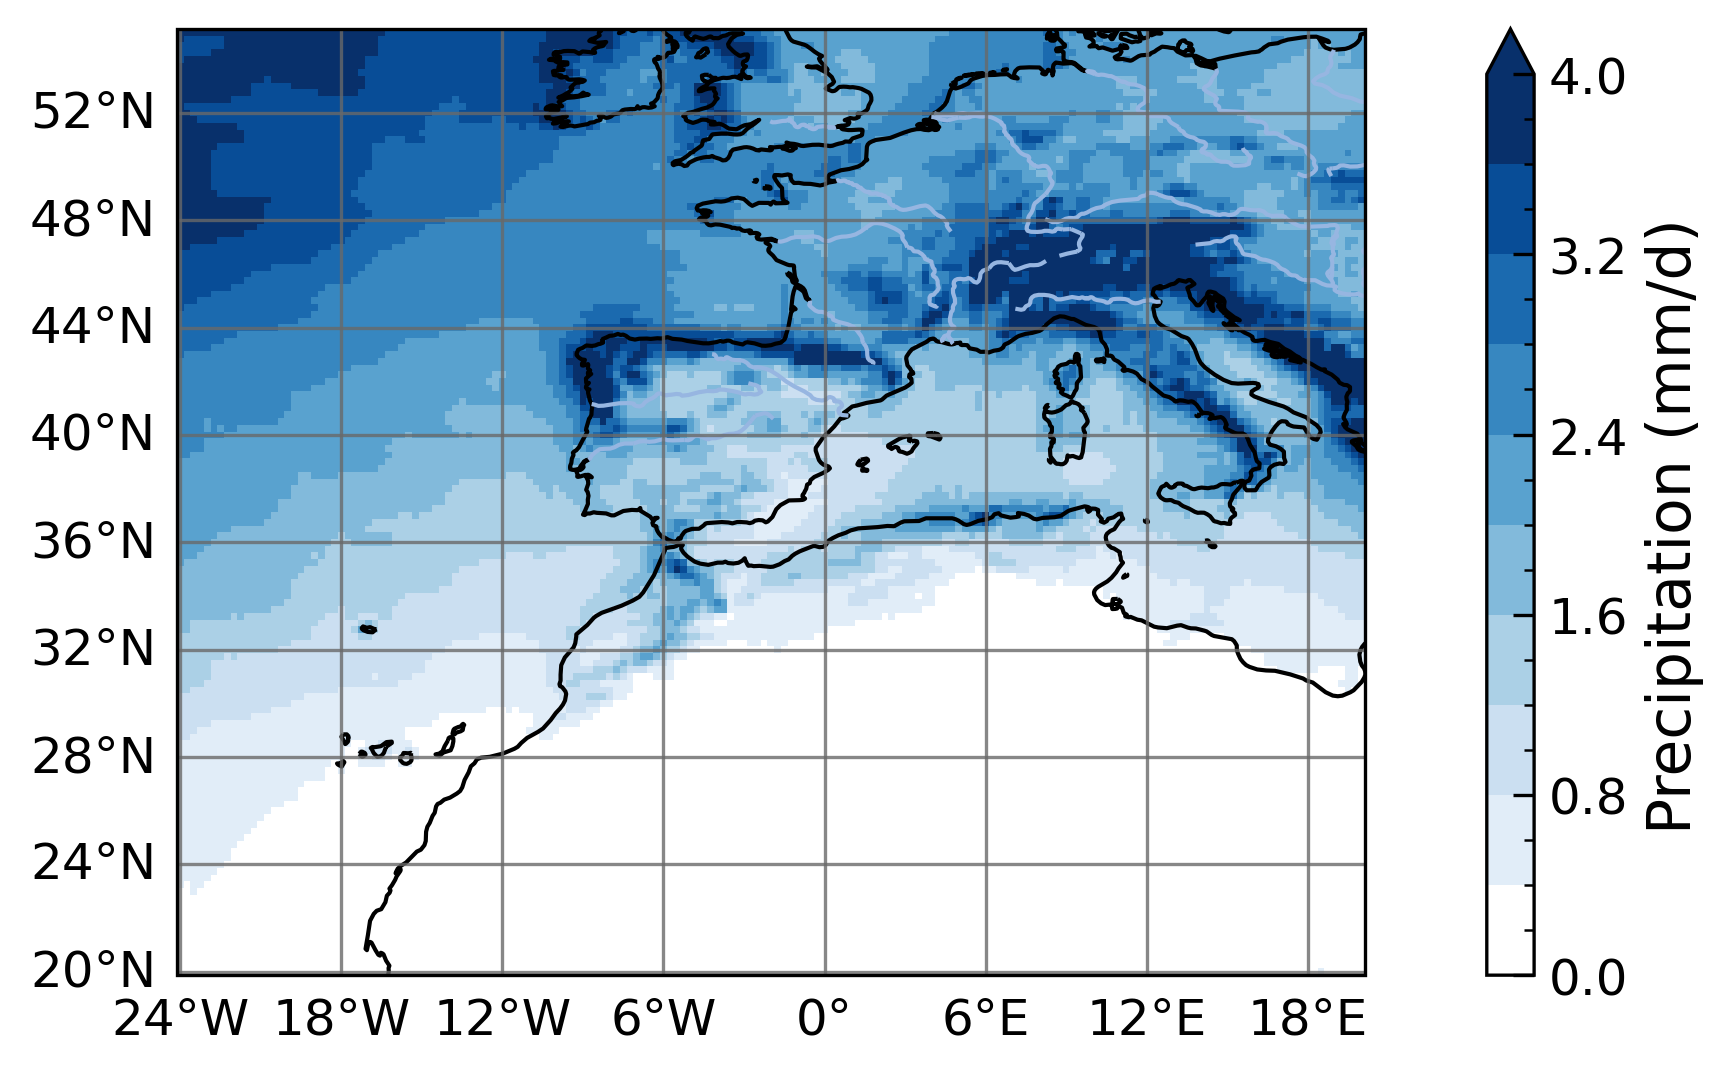
\includegraphics[width=\textwidth]{images/chap4/domain_size/var_map_precip_ERA5.png}
        \end{subfigure} &
        \begin{subfigure}[b]{0.33\textwidth}
            \caption{Downwelling shortwave \\radiation (W \persqm)}
            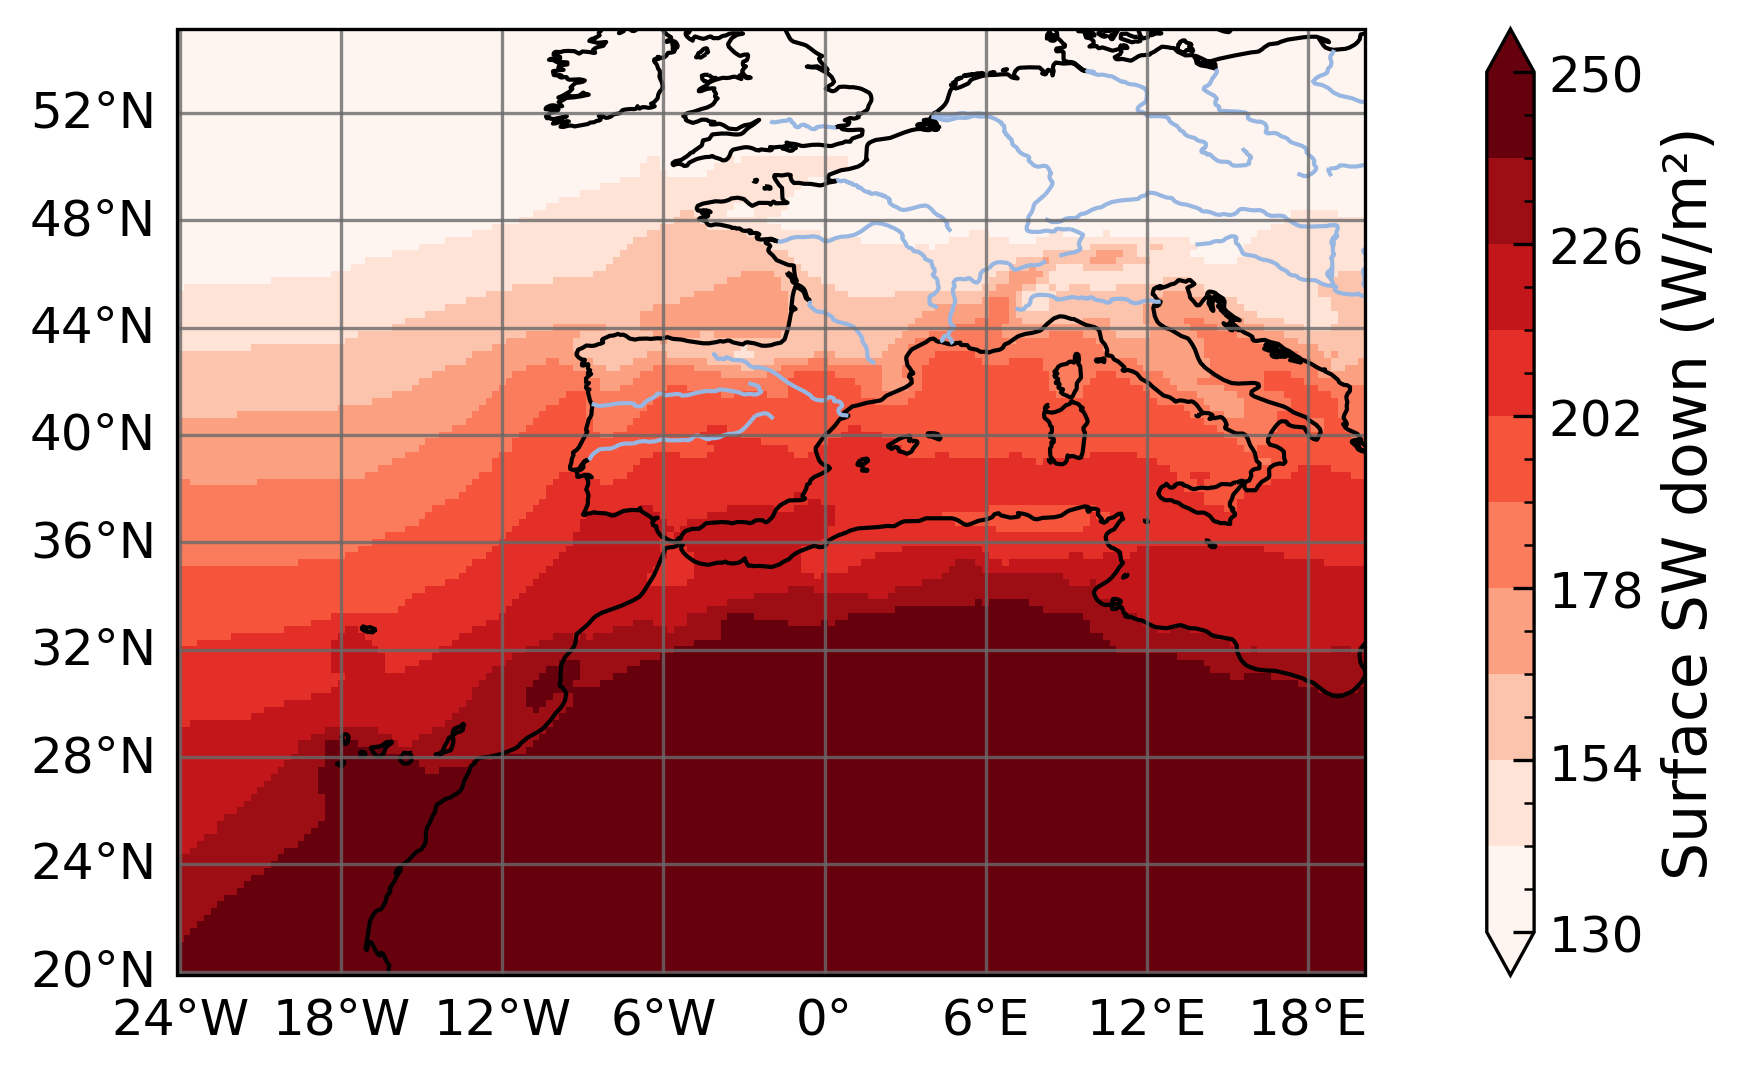
\includegraphics[width=\textwidth]{images/chap4/domain_size/var_map_SWdnSFC_ERA5.png}
        \end{subfigure} &
        \begin{subfigure}[b]{0.33\textwidth}
            \caption{Total cloud cover \\(sky fraction in \%)}
            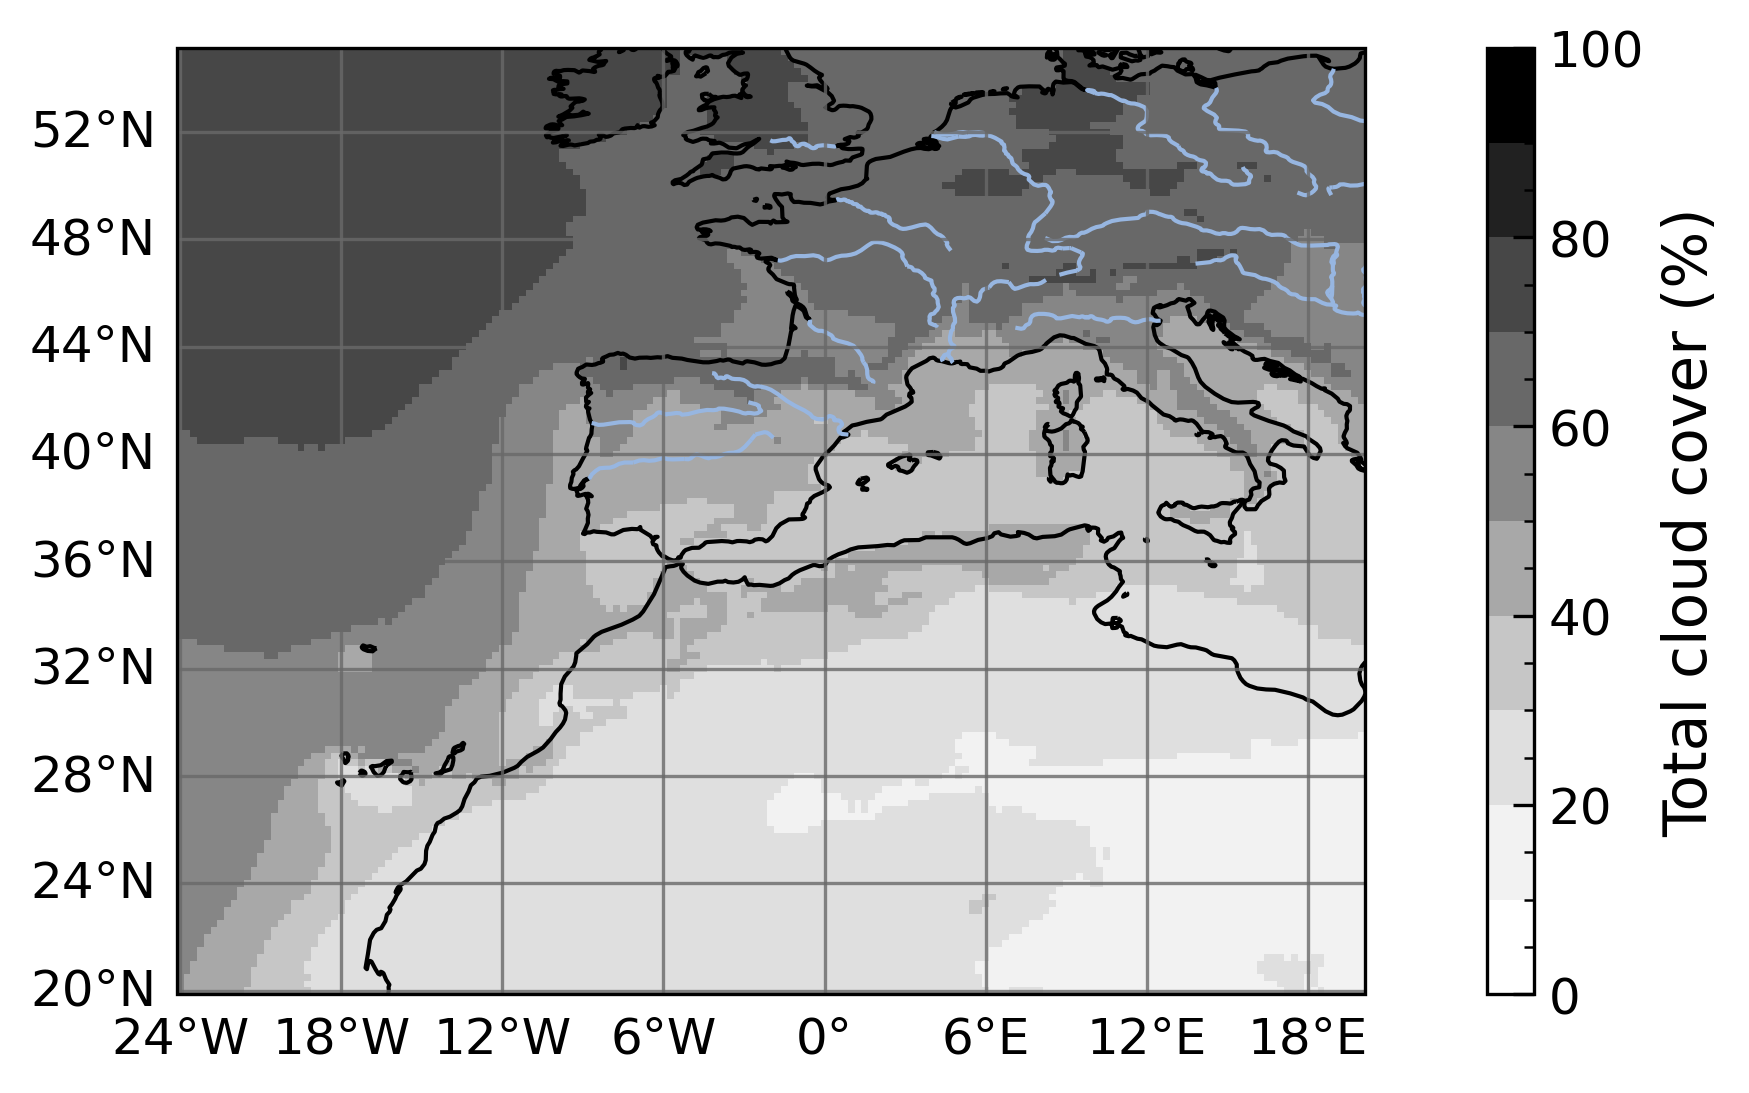
\includegraphics[width=\textwidth]{images/chap4/domain_size/var_map_cldt_ERA5.png}
        \end{subfigure} \\

        \begin{subfigure}[b]{0.33\textwidth}
            \caption{Evapotranspiration (mm \perday)}
            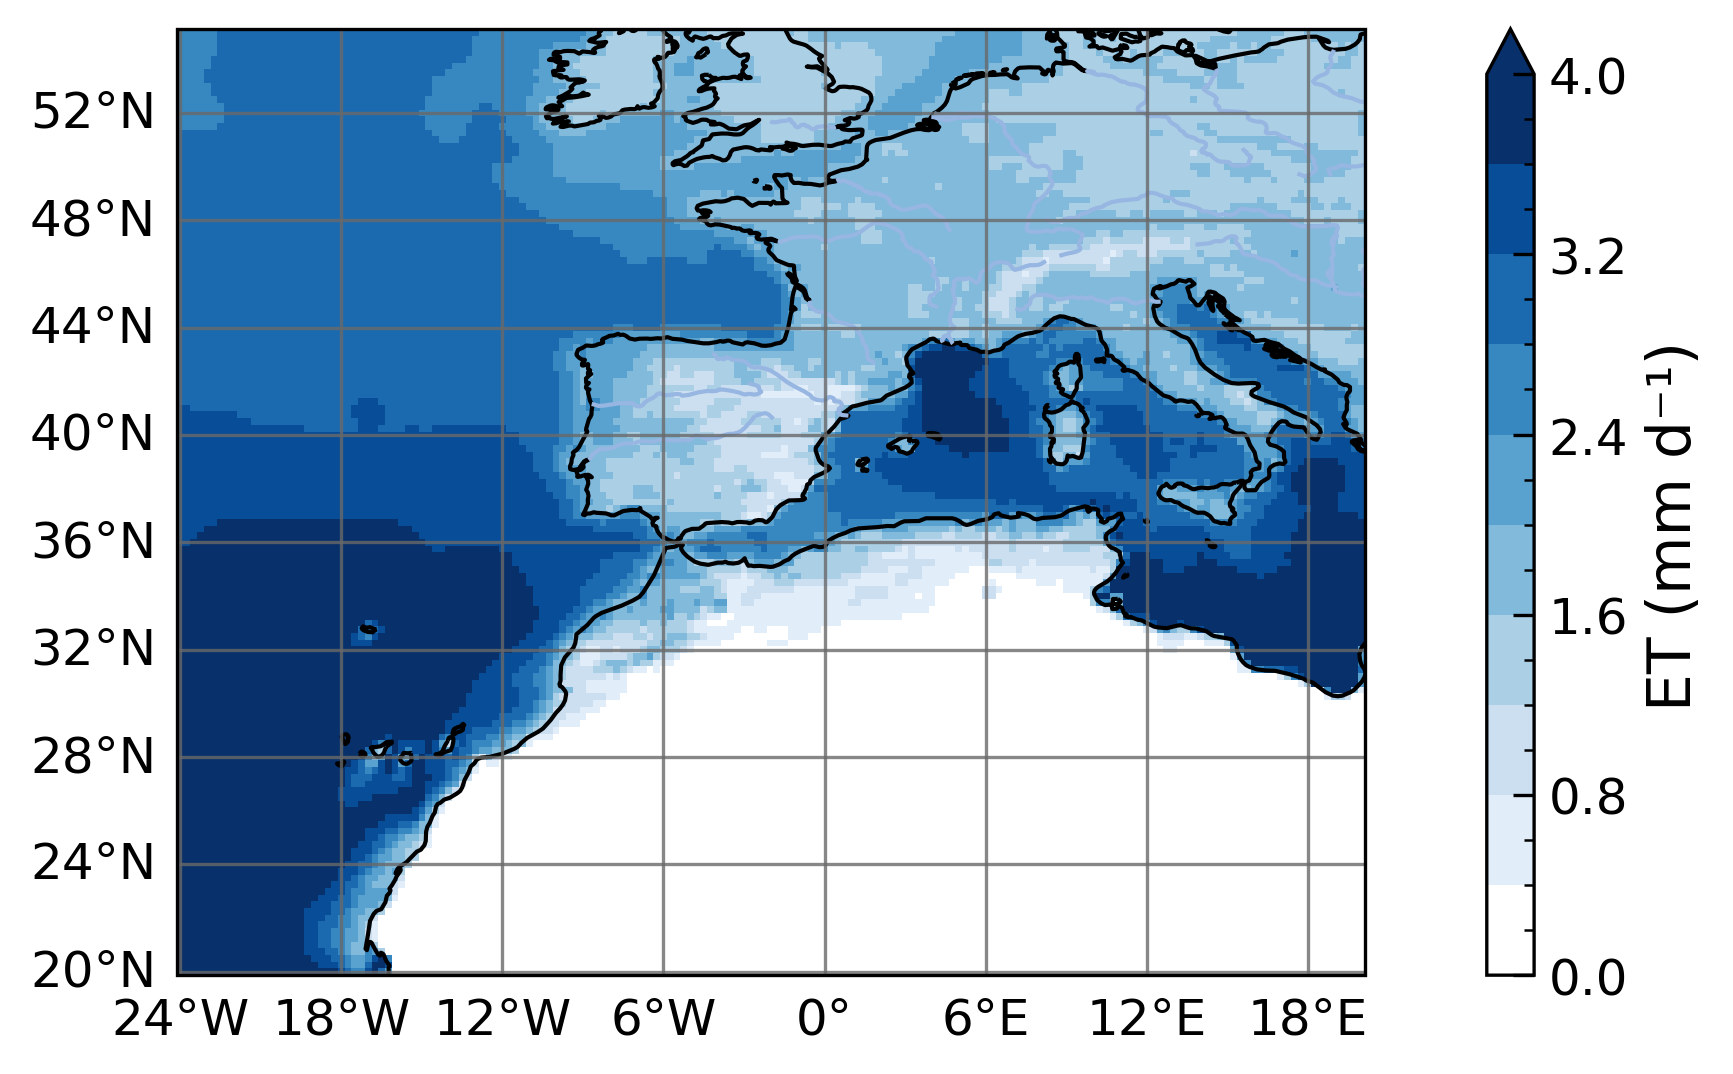
\includegraphics[width=\textwidth]{images/chap4/domain_size/var_map_evap_ERA5.png}
        \end{subfigure} &
        \begin{subfigure}[b]{0.33\textwidth}
            \caption{Downwelling longwave \\radiation (W \persqm)}
            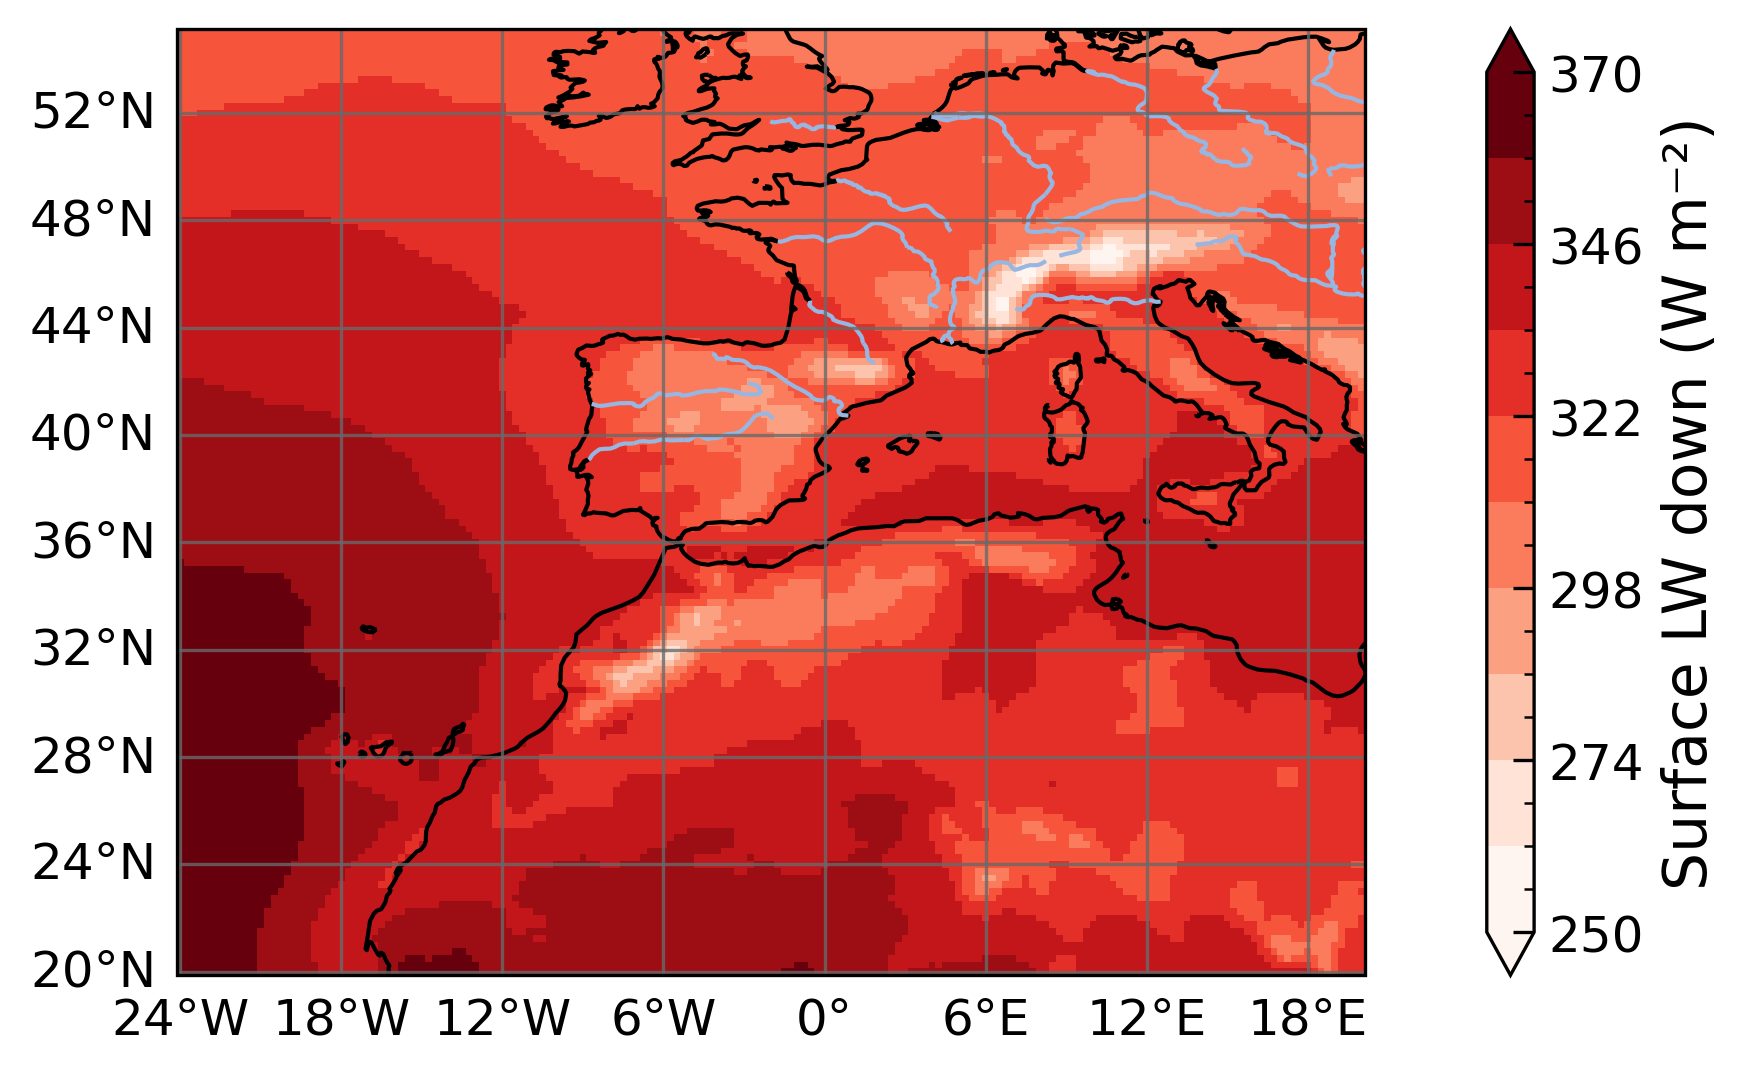
\includegraphics[width=\textwidth]{images/chap4/domain_size/var_map_LWdnSFC_ERA5.png}
        \end{subfigure} &
        \begin{subfigure}[b]{0.33\textwidth}
            \caption{Low cloud cover \\(sky fraction in \%)}
            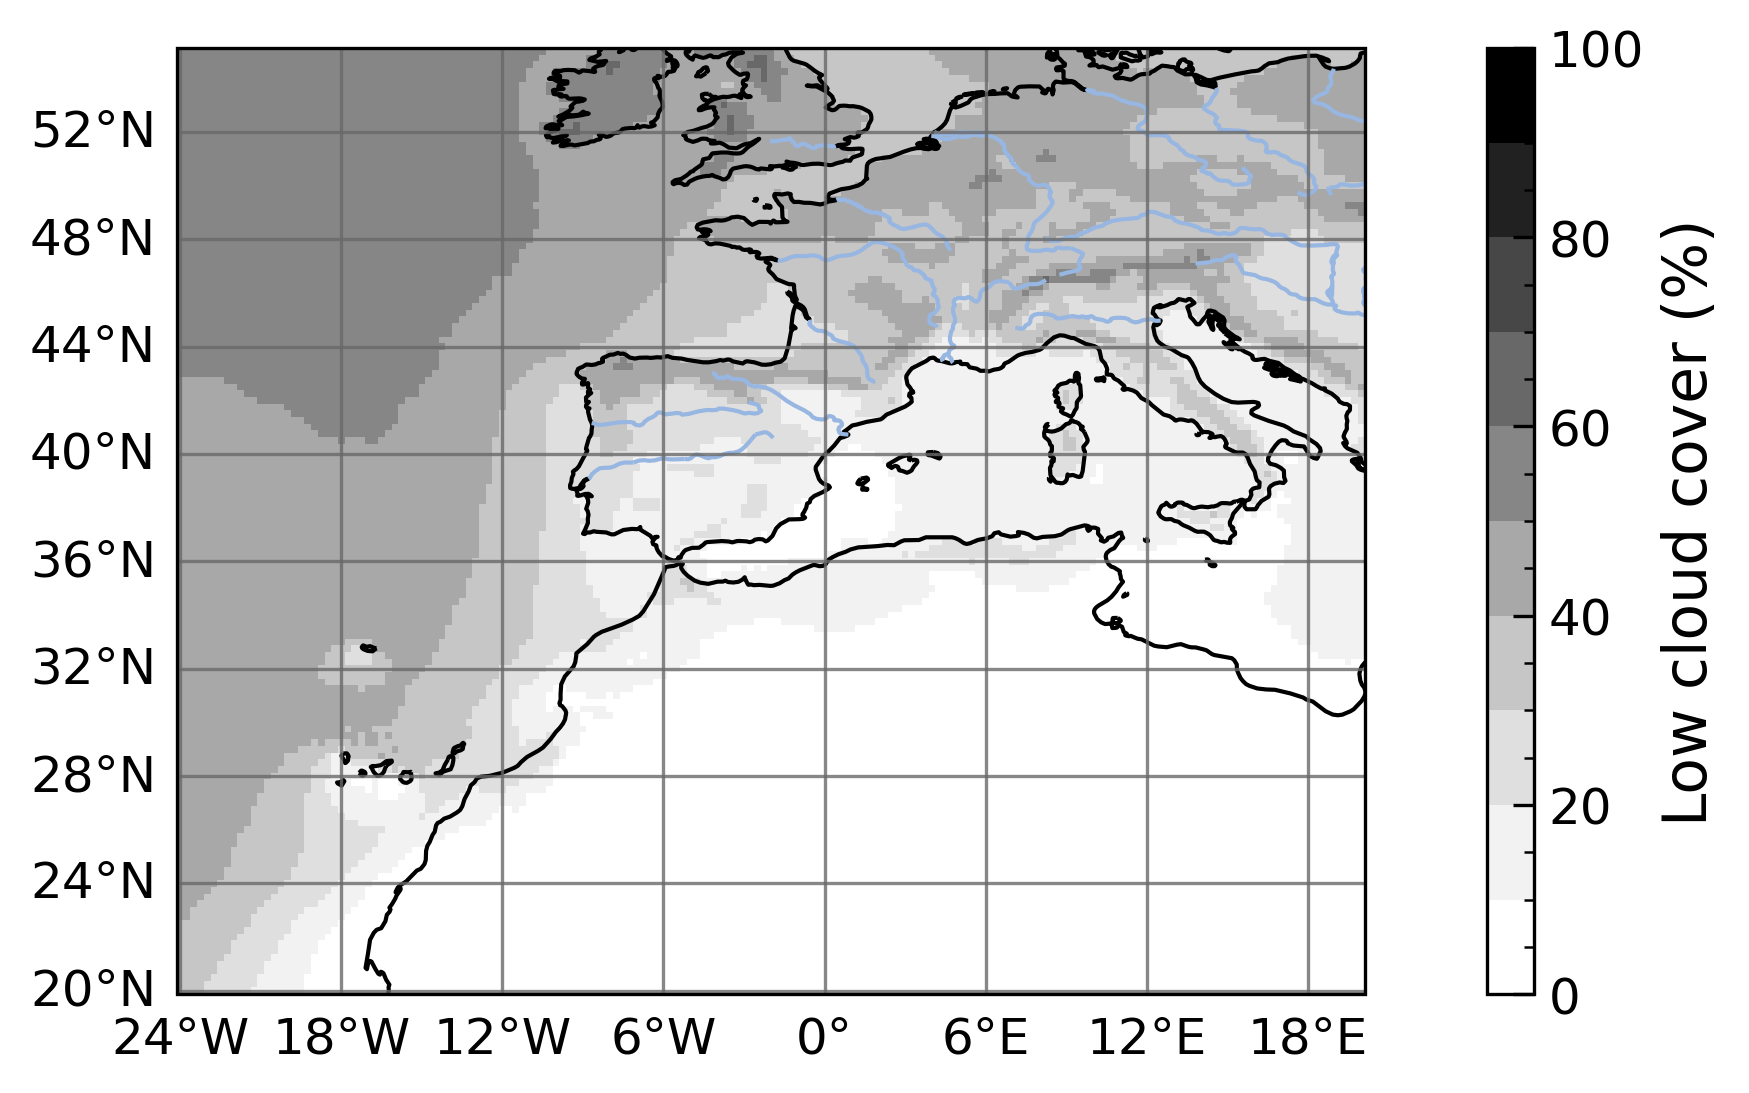
\includegraphics[width=\textwidth]{images/chap4/domain_size/var_map_cldl_ERA5.png}
        \end{subfigure}
    \end{tabular}
    \caption{Annual mean of the six variables of interest for the analysis of the LAM structural biases in ERA5 over the period 2010-2014.}
    \label{fig:ERA_var_maps}
\end{figure}

\section{Structural inconsistencies and influence of domain size}
\label{sec:domain_size}
Here, three simulations over the periods 2010-2014 are compared to ERA5:
\begin{itemize}
    \item \smalld : $R_{domain} = 1000 km$, $NBP=40$
    \item \interd : $R_{domain} = 1500 km$, $NBP=60$
    \item \larged : $R_{domain} = 2000 km$, , $NBP=80$
\end{itemize}

The inconsistencies were identified with the initial simulation setup \smalld, by noticing that there was little to no precipitation on the edges of the domain. The LAM presented a strong underestimation compared to ERA5 in the transition zone (Fig. \ref{fig:domain_size_P_ET_ERA_diff_maps}a), but it remained hard to know if these biases had an influence on the rest of the domain, and particularly on the Iberian Peninsula, which also exhibited underestimated precipitation in its northern and western coasts.
This lack of precipitation appeared to lead to a lower ET on continents which received less water. However, over the Atlantic ocean and the Mediterranean sea, ET was surprisingly high, overestimating the values of ERA5 (Fig. \ref{fig:domain_size_P_ET_ERA_diff_maps}b). 

Simulations with the intermediate and large domains showed that the bias in precipitation was mostly located in the transition zone, especially in the northwest of the domain which is not influenced by the presence of continents, and decreased towards the center. 
The differences compared to ERA5 in the transition zone correspond to a relative decrease between -80\% and -100\%, meaning the model computes almost no precipitation in these grid cells (Fig. \ref{fig:domain_size_ERA_reldiff_maps}).
In the free zone, precipitation remains underestimated in the northern coast of the Peninsula, but it does not seem to result from the behaviour of the model on the edges of the domain.
The overestimation in ET is also confined to the northwestern edge of the domain and the large overestimation in the Mediterranean is reversed to an underestimation of smaller magnitude.
As mentionned before, although ERA5 cannot be considered as the best reference product for all the variables considered, it is the spatial structure of the biases that is striking here, since they are independent of the structure of the variable (Fig. \ref{fig:ERA_var_maps}), and follow the edges of the domain even when the radius changes.

%figure : maps of diff vs ERA for 3 domain sizes : precip, evap
\begin{figure}[htbp]
    \centering
    \begin{tabular}{ccc}
        %precip
        \begin{subfigure}[b]{0.33\textwidth}
            \caption{Precipitation bias to ERA5\\(mm \perday, \smalld)}
            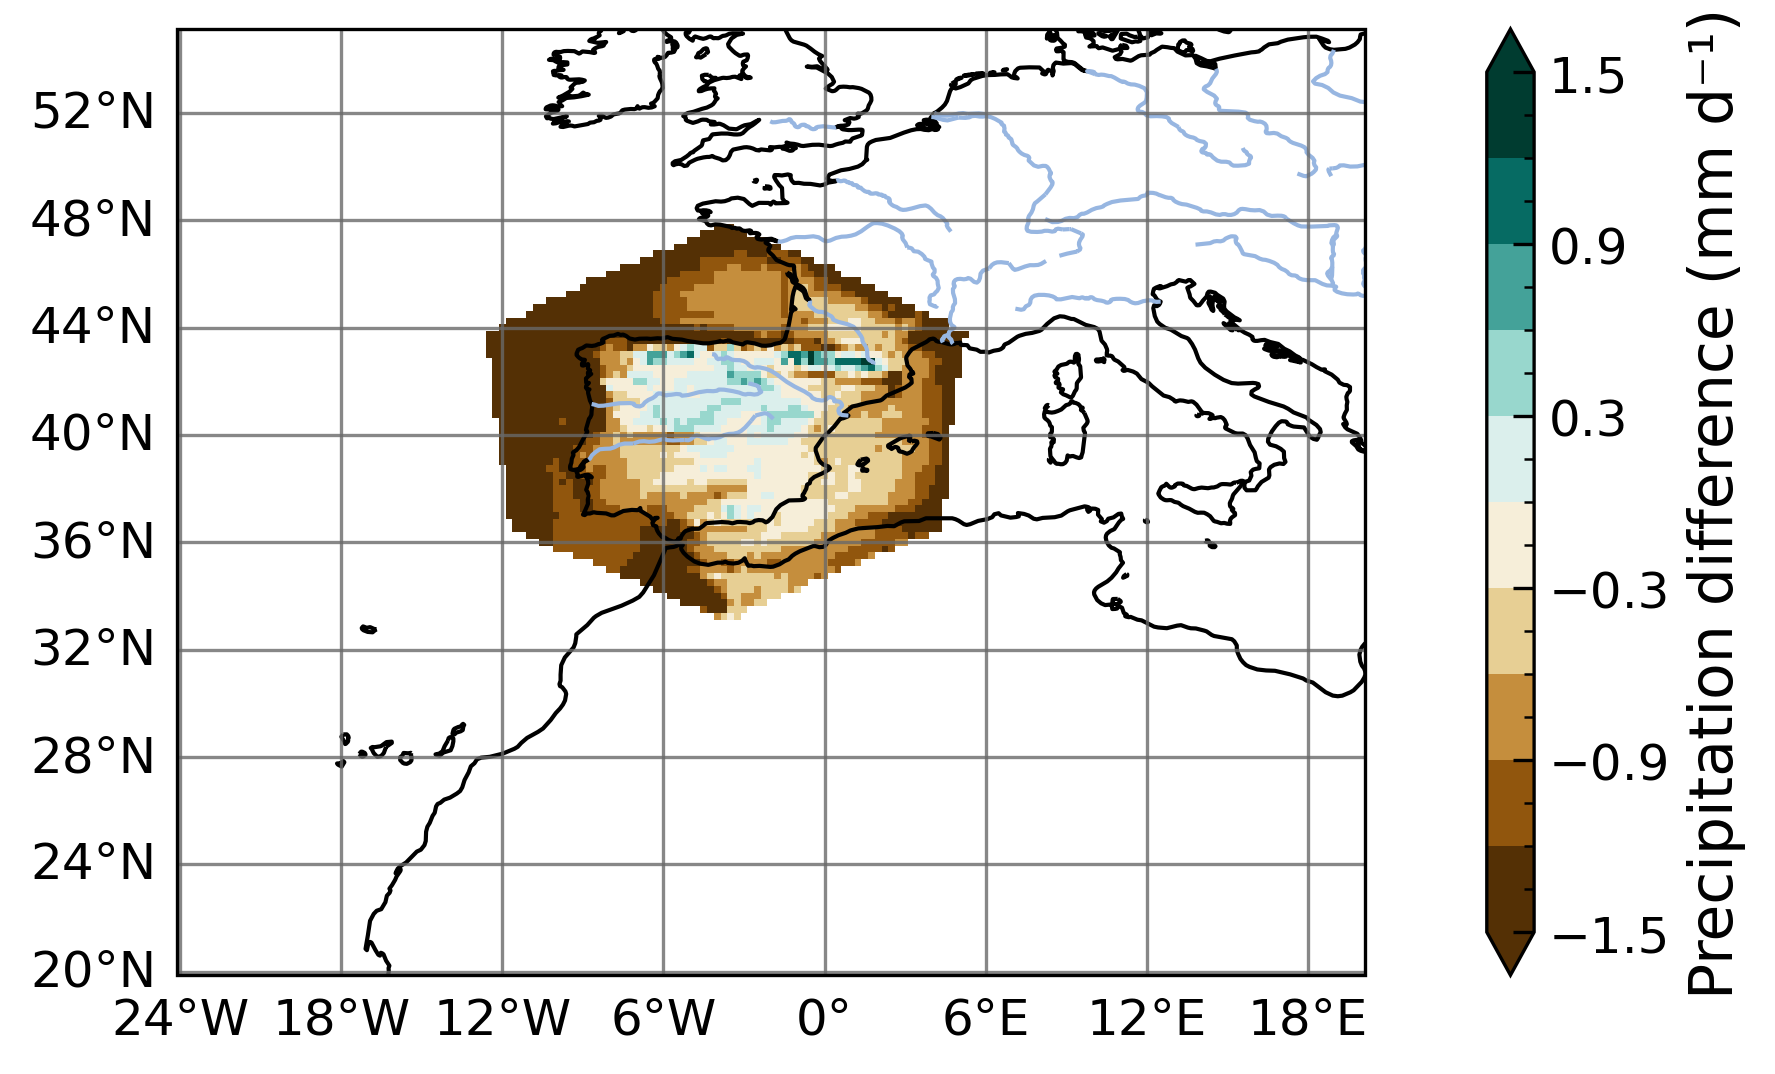
\includegraphics[width=\textwidth]{images/chap4/domain_size/diff_map_precip_era_LAM_1000km_NBP40.png}
        \end{subfigure} &
        \begin{subfigure}[b]{0.33\textwidth}
            \caption{Precipitation bias to ERA5\\(mm \perday, \interd)}
            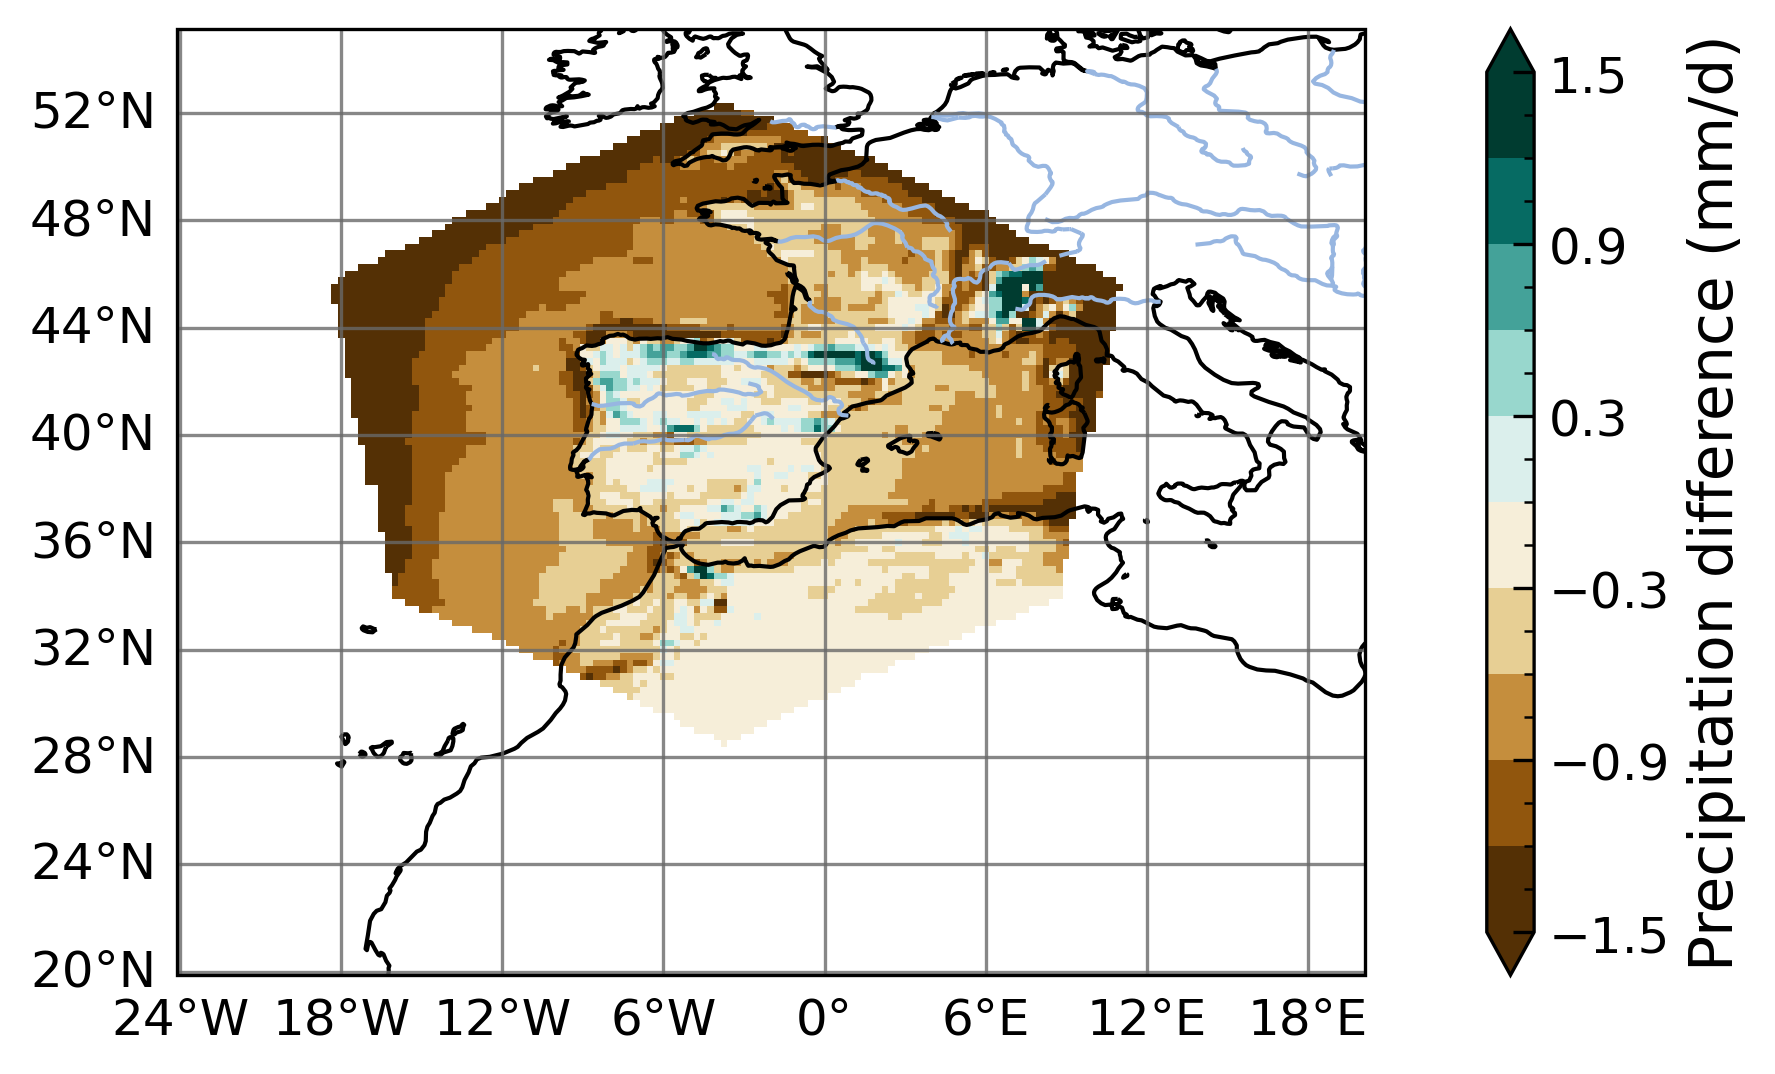
\includegraphics[width=\textwidth]{images/chap4/domain_size/diff_map_precip_era_LAM_1500km_NBP60.png}
        \end{subfigure} &
        \begin{subfigure}[b]{0.33\textwidth}
            \caption{Precipitation bias to ERA5 \\(mm \perday, \larged)}
            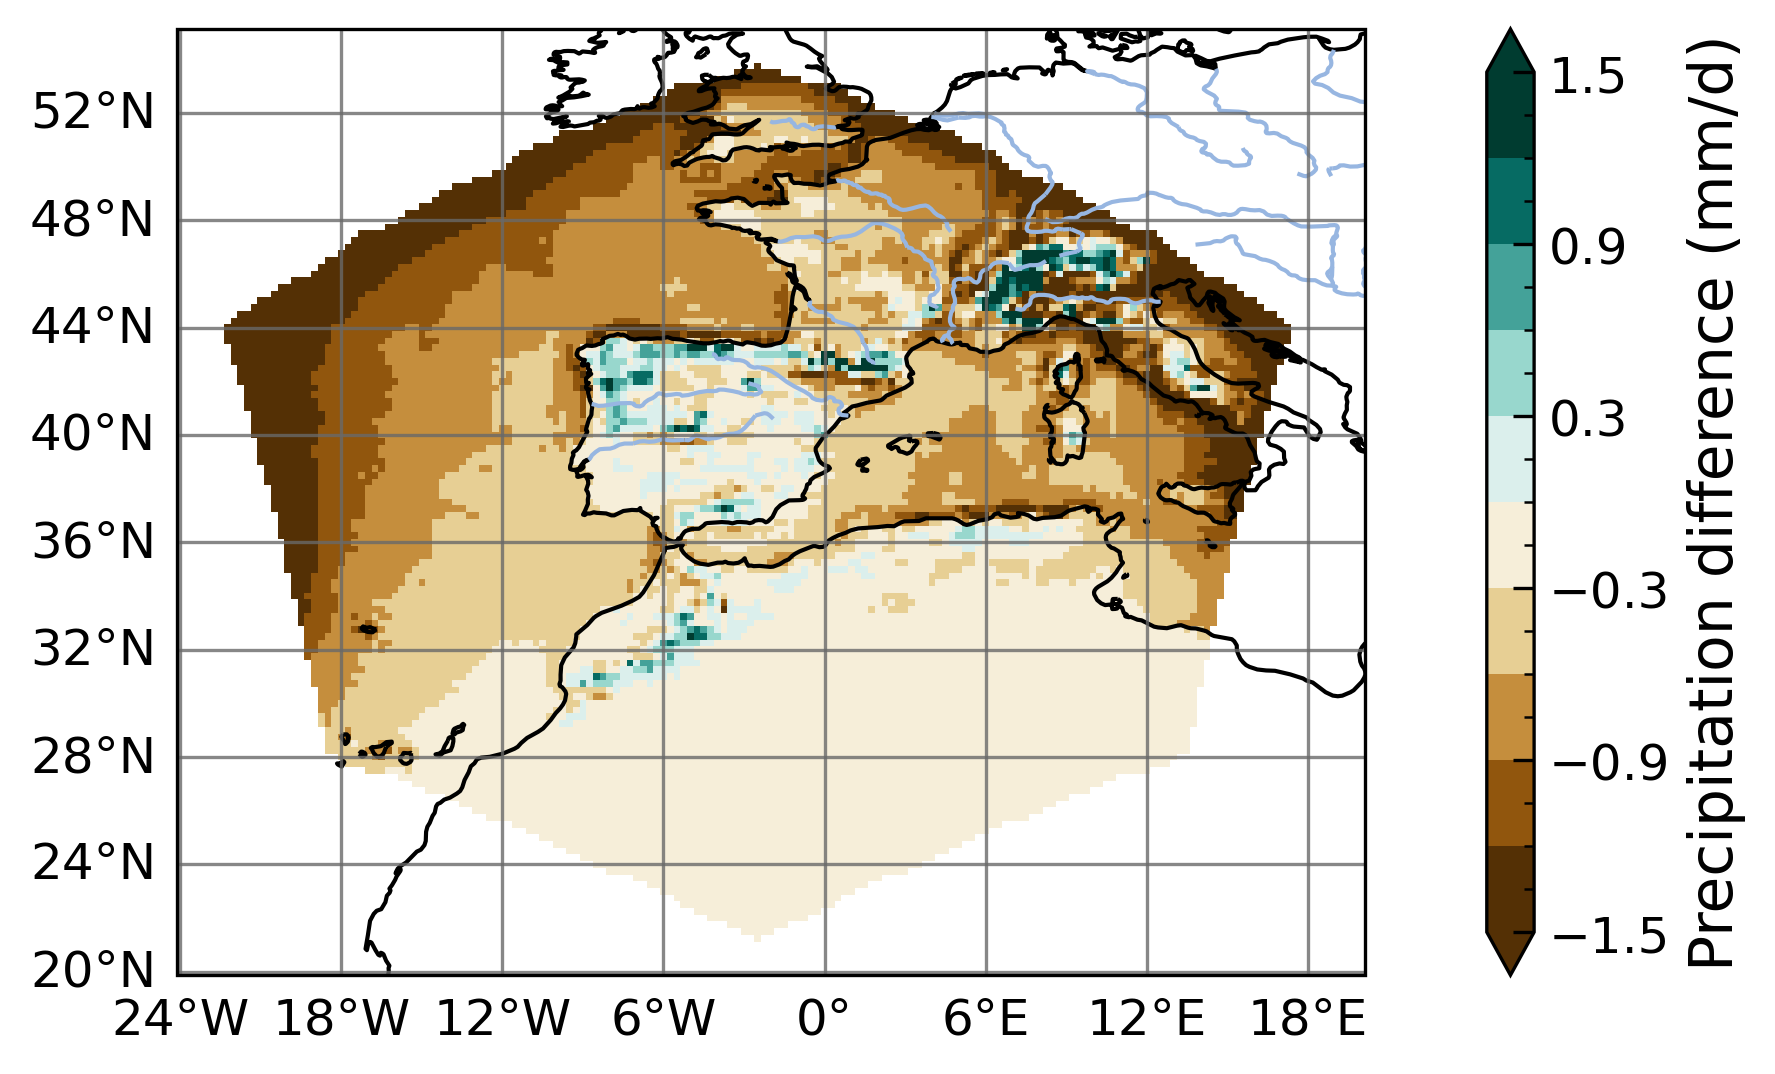
\includegraphics[width=\textwidth]{images/chap4/domain_size/diff_map_precip_era_LAM_2000km_NBP80.png}
        \end{subfigure} \\
        
        %evap
        \begin{subfigure}[b]{0.33\textwidth}
            \caption{ET bias to ERA5\\(mm \perday, \smalld)}
            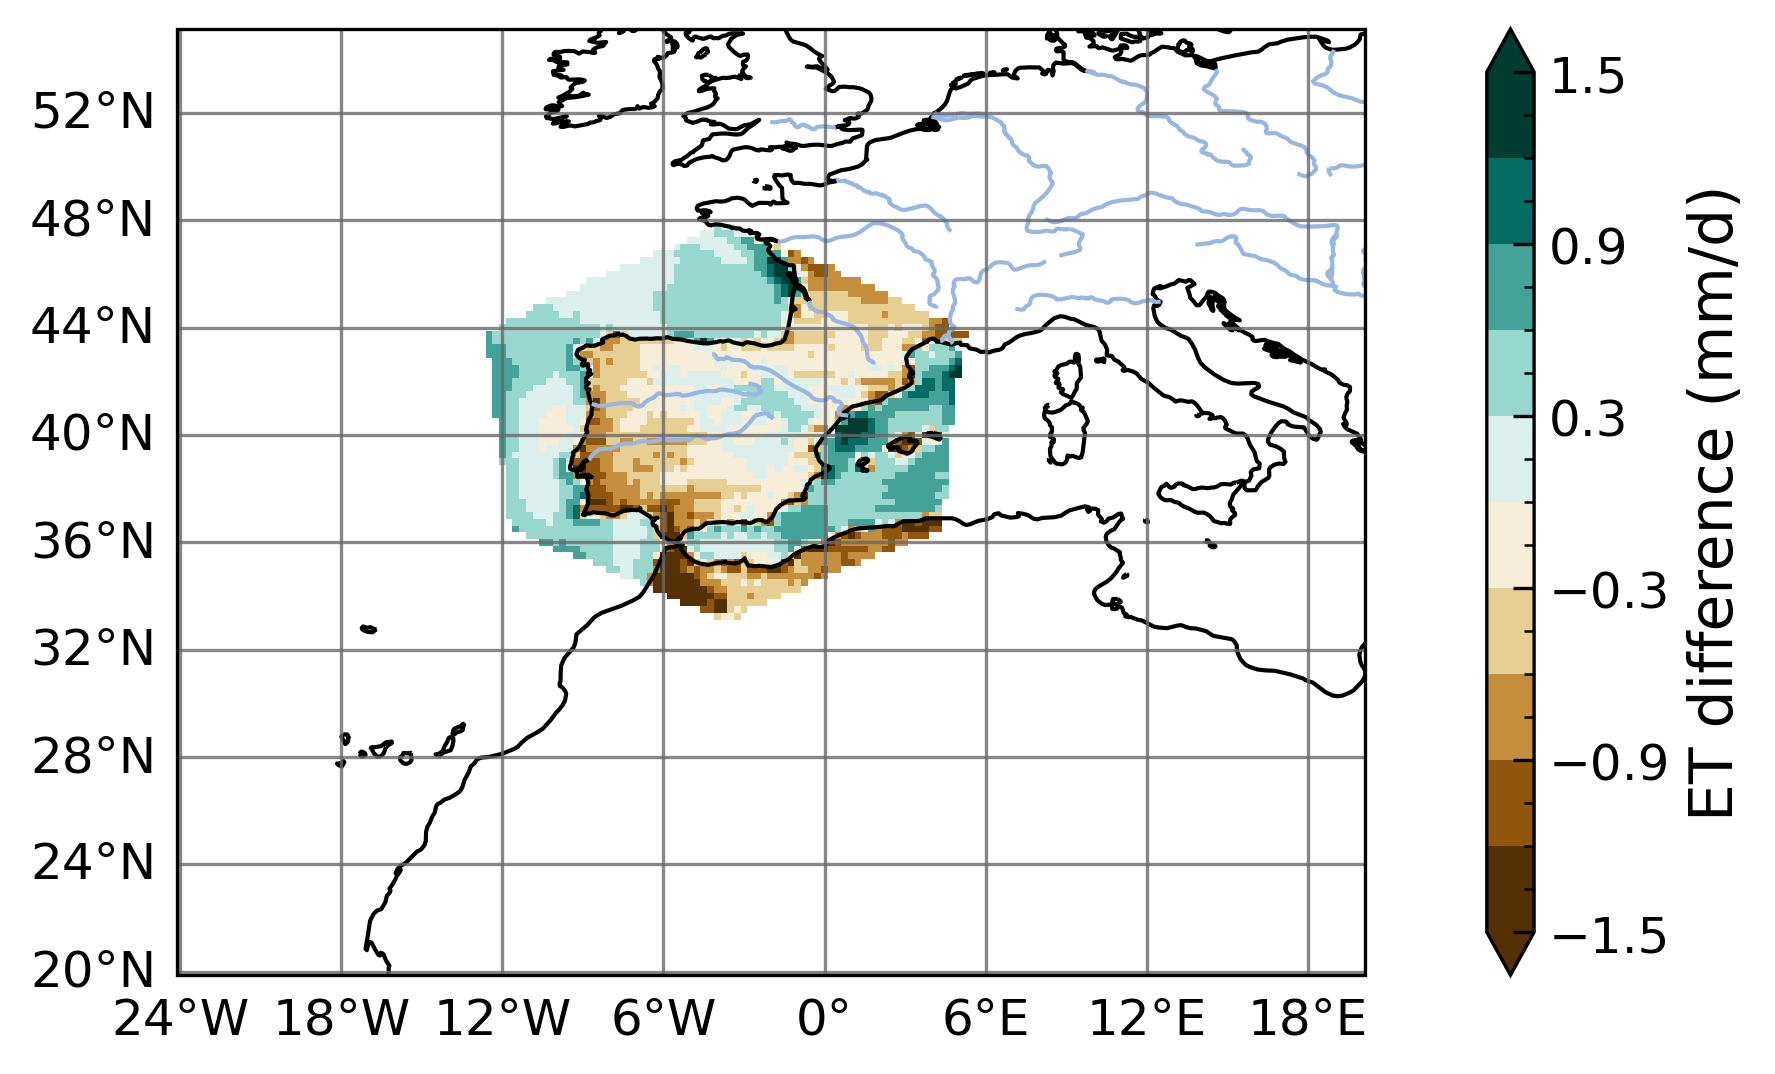
\includegraphics[width=\textwidth]{images/chap4/domain_size/diff_map_evap_era_LAM_1000km_NBP40.png}
        \end{subfigure} &
        \begin{subfigure}[b]{0.33\textwidth}
            \caption{ET bias to ERA5\\(mm \perday, \interd)}
            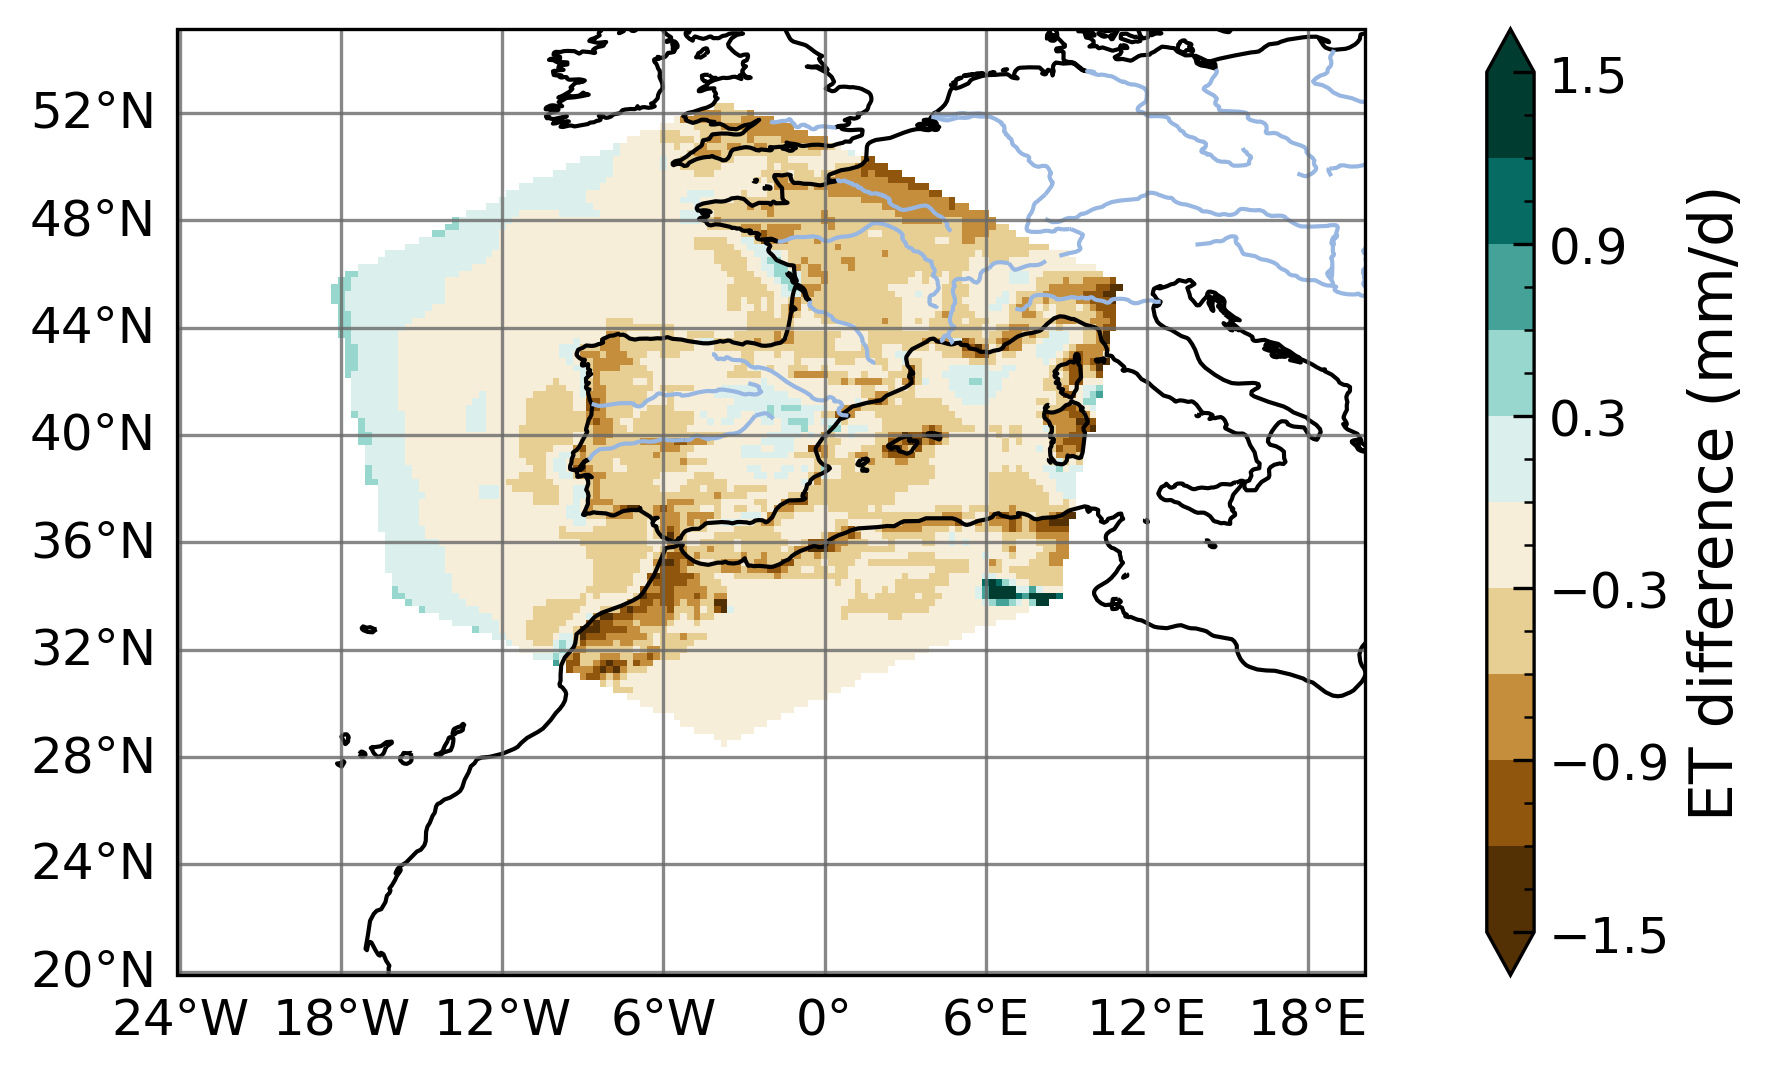
\includegraphics[width=\textwidth]{images/chap4/domain_size/diff_map_evap_era_LAM_1500km_NBP60.png}
        \end{subfigure} &
        \begin{subfigure}[b]{0.33\textwidth}
            \caption{ET bias to ERA5\\(mm \perday, \larged)}
            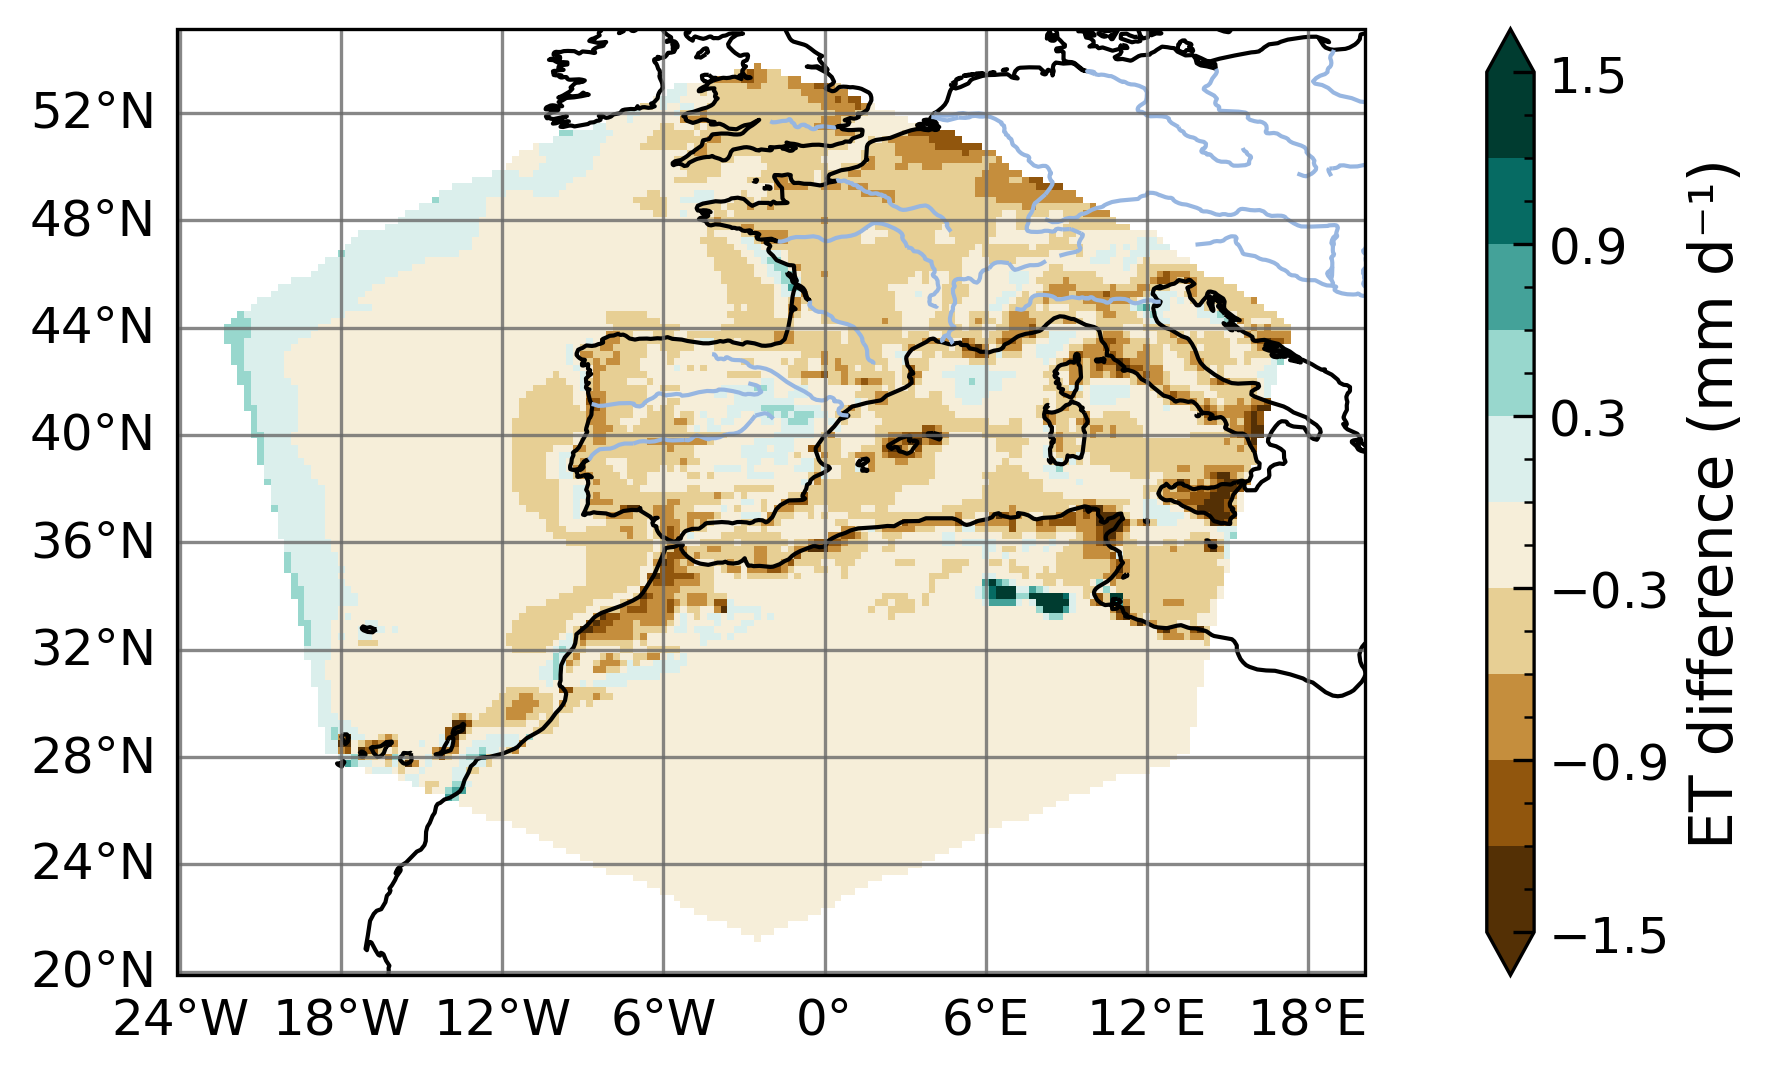
\includegraphics[width=\textwidth]{images/chap4/domain_size/diff_map_evap_era_LAM_2000km_NBP80.png}
        \end{subfigure} 
    \end{tabular}
    \caption{Precipitation and evapotranspiration biases compared to ERA5 over 2010-2014 for three simulations with small, intermediate and large domain sizes.}
    \label{fig:domain_size_P_ET_ERA_diff_maps}
\end{figure}

These first findings led to the hypothesis that the physics of the LAM were not behaving in a normal way in the transition zone, and more specifically the large-scale water condensation scheme. 
Comparisons with ERA5 show an underestimation of total cloud cover in the transition zone (Fig. \ref{fig:domain_size_clouds_ERA_diff_maps}a-c) and particularly of low cloud cover (Fig. \ref{fig:domain_size_clouds_ERA_diff_maps}d-f), which constitutes its most important component (Fig. \ref{fig:ERA_var_maps}c,f).
The absence of clouds allows more incoming solar radiation to reach the surface, leading to higher values of the downwelling shortwave radiation flux (Fig. \ref{fig:domain_size_clouds_ERA_diff_maps}g-i). This can explain the higher ET values since it provides more available energy for evaporation of seawater.
Having less condensed water also leads to a smaller downwelling longwave radiation flux in the transition zone (Fig. \ref{fig:domain_size_clouds_ERA_diff_maps}j-l). This is consistent with the bias for this variable in the central part of the domain, where it is overestimated, following the spatial patterns seen for low cloud cover.


%figure : maps of diff vs ERA for 3 domain sizes : SW, LW, cloud cover
\begin{figure}[htbp]
    \centering
    \begin{tabular}{ccc}
        %total
        \begin{subfigure}[b]{0.33\textwidth}
            \caption{Total cloud cover bias\\(\% of sky, \smalld)}
            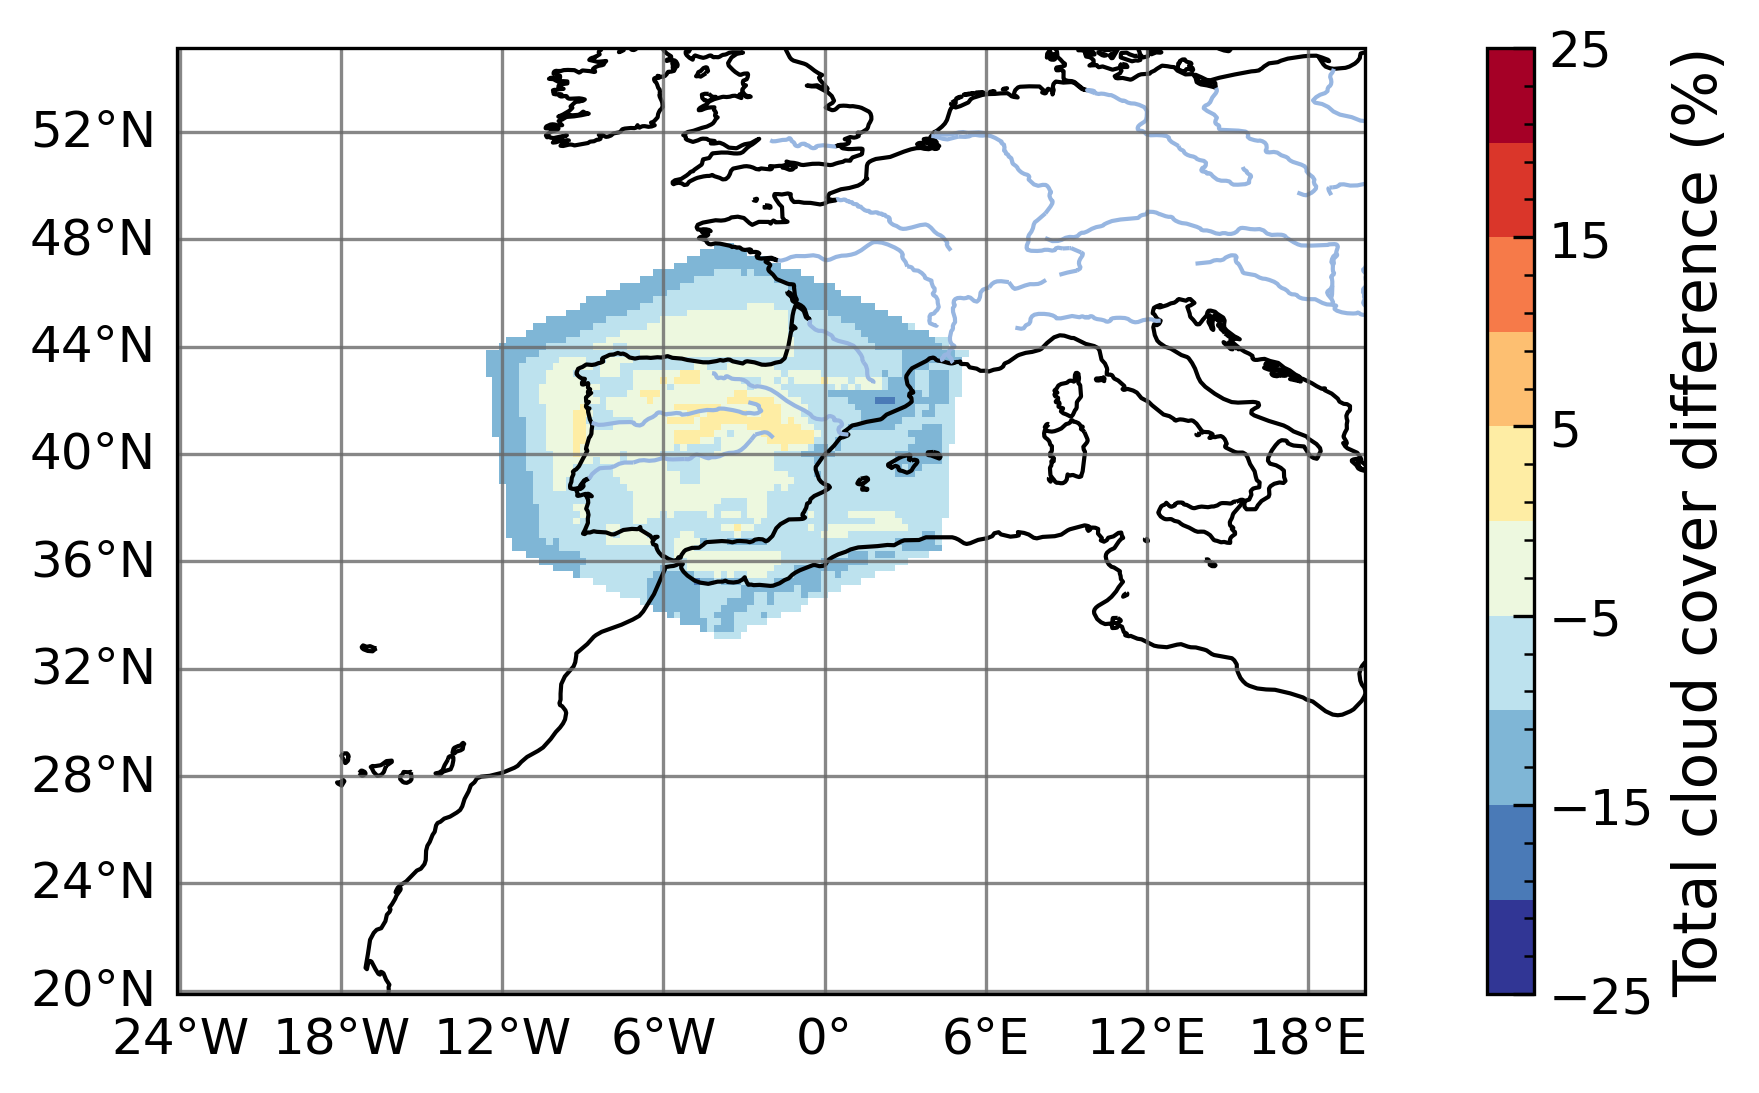
\includegraphics[width=\textwidth]{images/chap4/domain_size/diff_map_cldt_era_LAM_1000km_NBP40.png}
        \end{subfigure} &
        \begin{subfigure}[b]{0.33\textwidth}
            \caption{Total cloud cover bias\\(\% of sky, \interd)}
            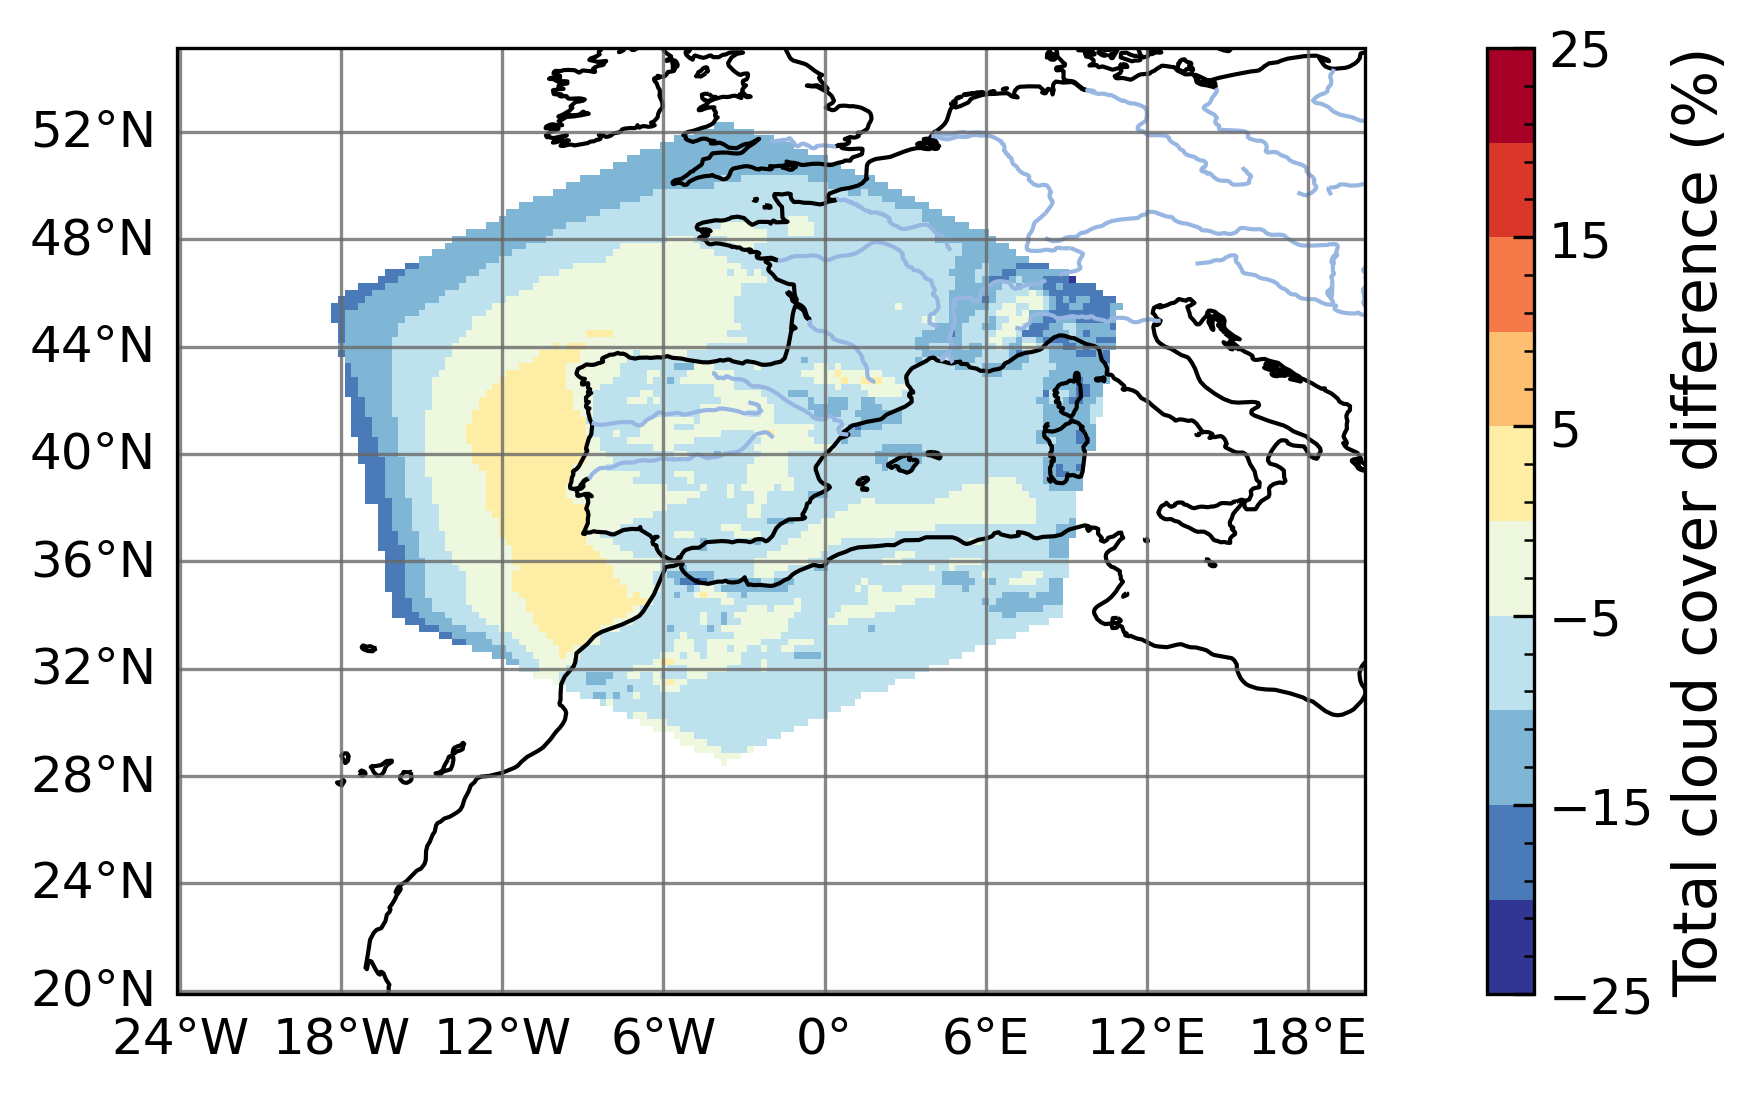
\includegraphics[width=\textwidth]{images/chap4/domain_size/diff_map_cldt_era_LAM_1500km_NBP60.png}
        \end{subfigure} &
        \begin{subfigure}[b]{0.33\textwidth}
            \caption{Total cloud cover bias\\(\% of sky, \larged)}
            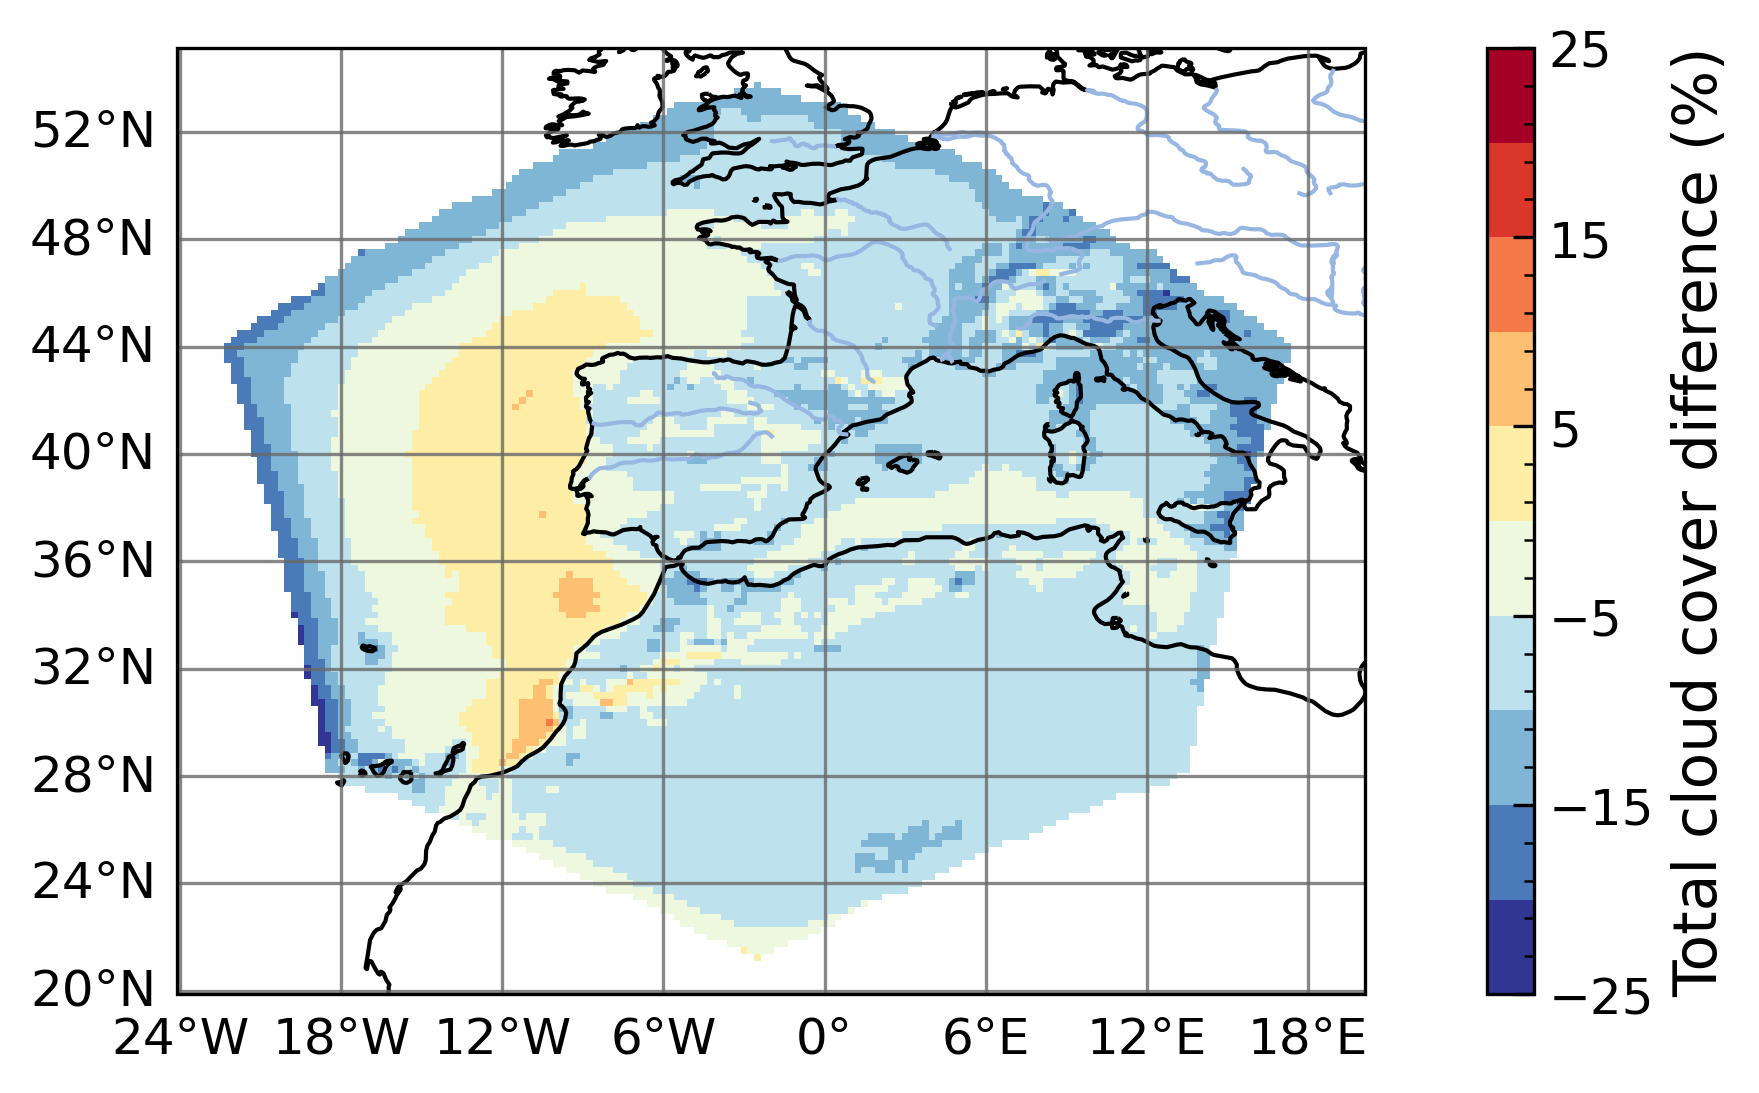
\includegraphics[width=\textwidth]{images/chap4/domain_size/diff_map_cldt_era_LAM_2000km_NBP80.png}
        \end{subfigure} \\
        
        %low
        \begin{subfigure}[b]{0.33\textwidth}
            \caption{Low cloud cover bias\\(\% of sky, \smalld)}
            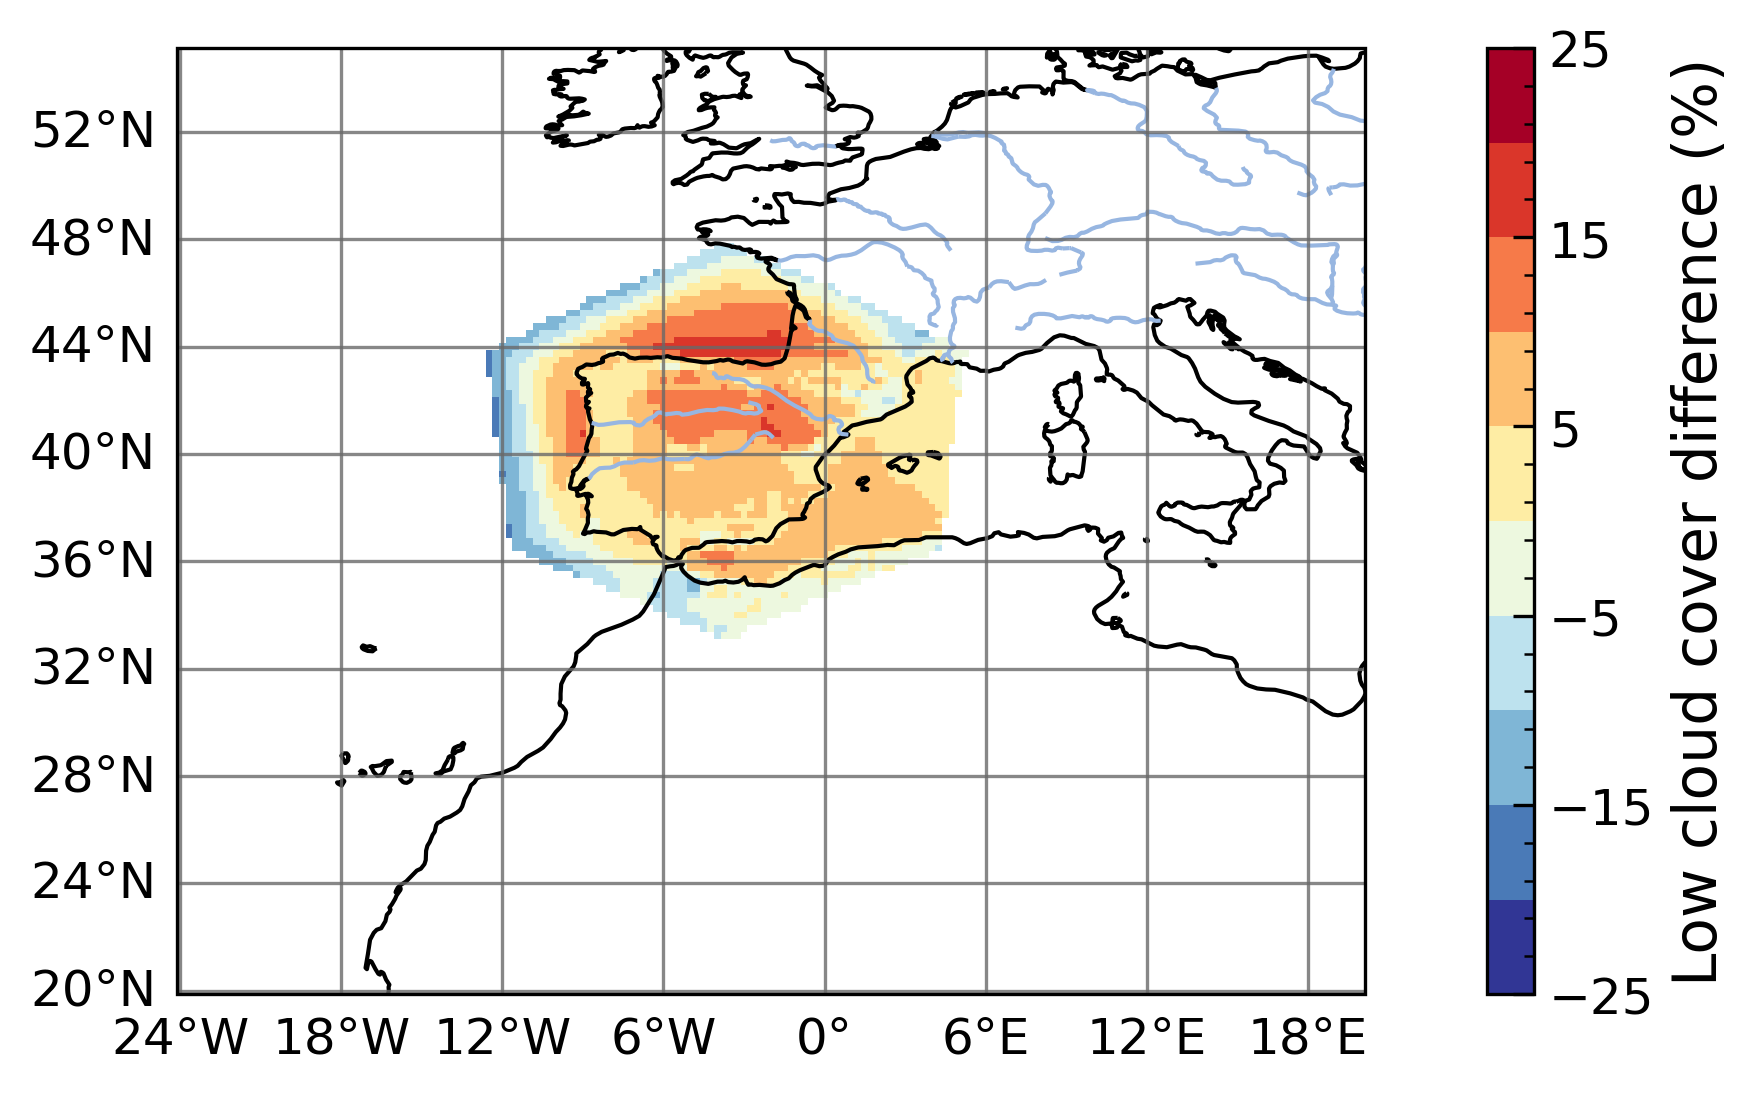
\includegraphics[width=\textwidth]{images/chap4/domain_size/diff_map_cldl_era_LAM_1000km_NBP40.png}
        \end{subfigure} &
        \begin{subfigure}[b]{0.33\textwidth}
            \caption{Low cloud cover bias\\(\% of sky, \interd)}
            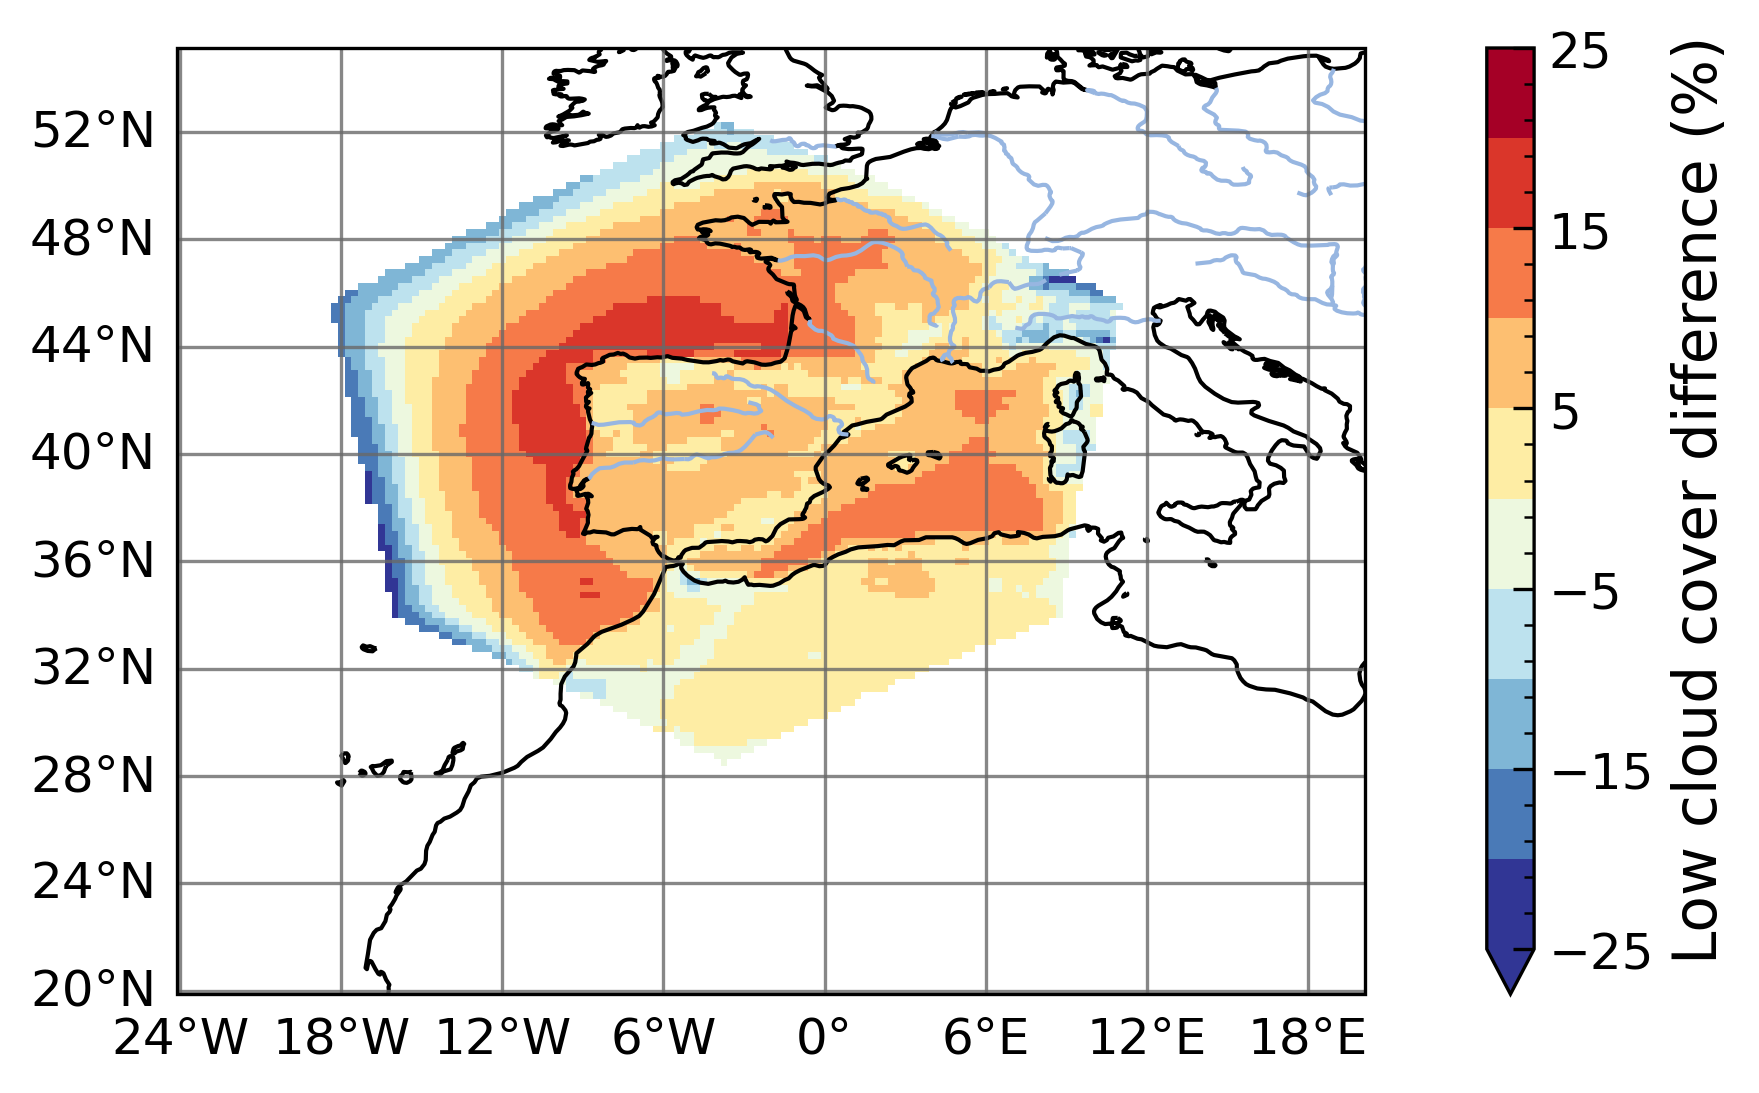
\includegraphics[width=\textwidth]{images/chap4/domain_size/diff_map_cldl_era_LAM_1500km_NBP60.png}
        \end{subfigure} &
        \begin{subfigure}[b]{0.33\textwidth}
            \caption{Low cloud cover bias\\(\% of sky, \larged)}
            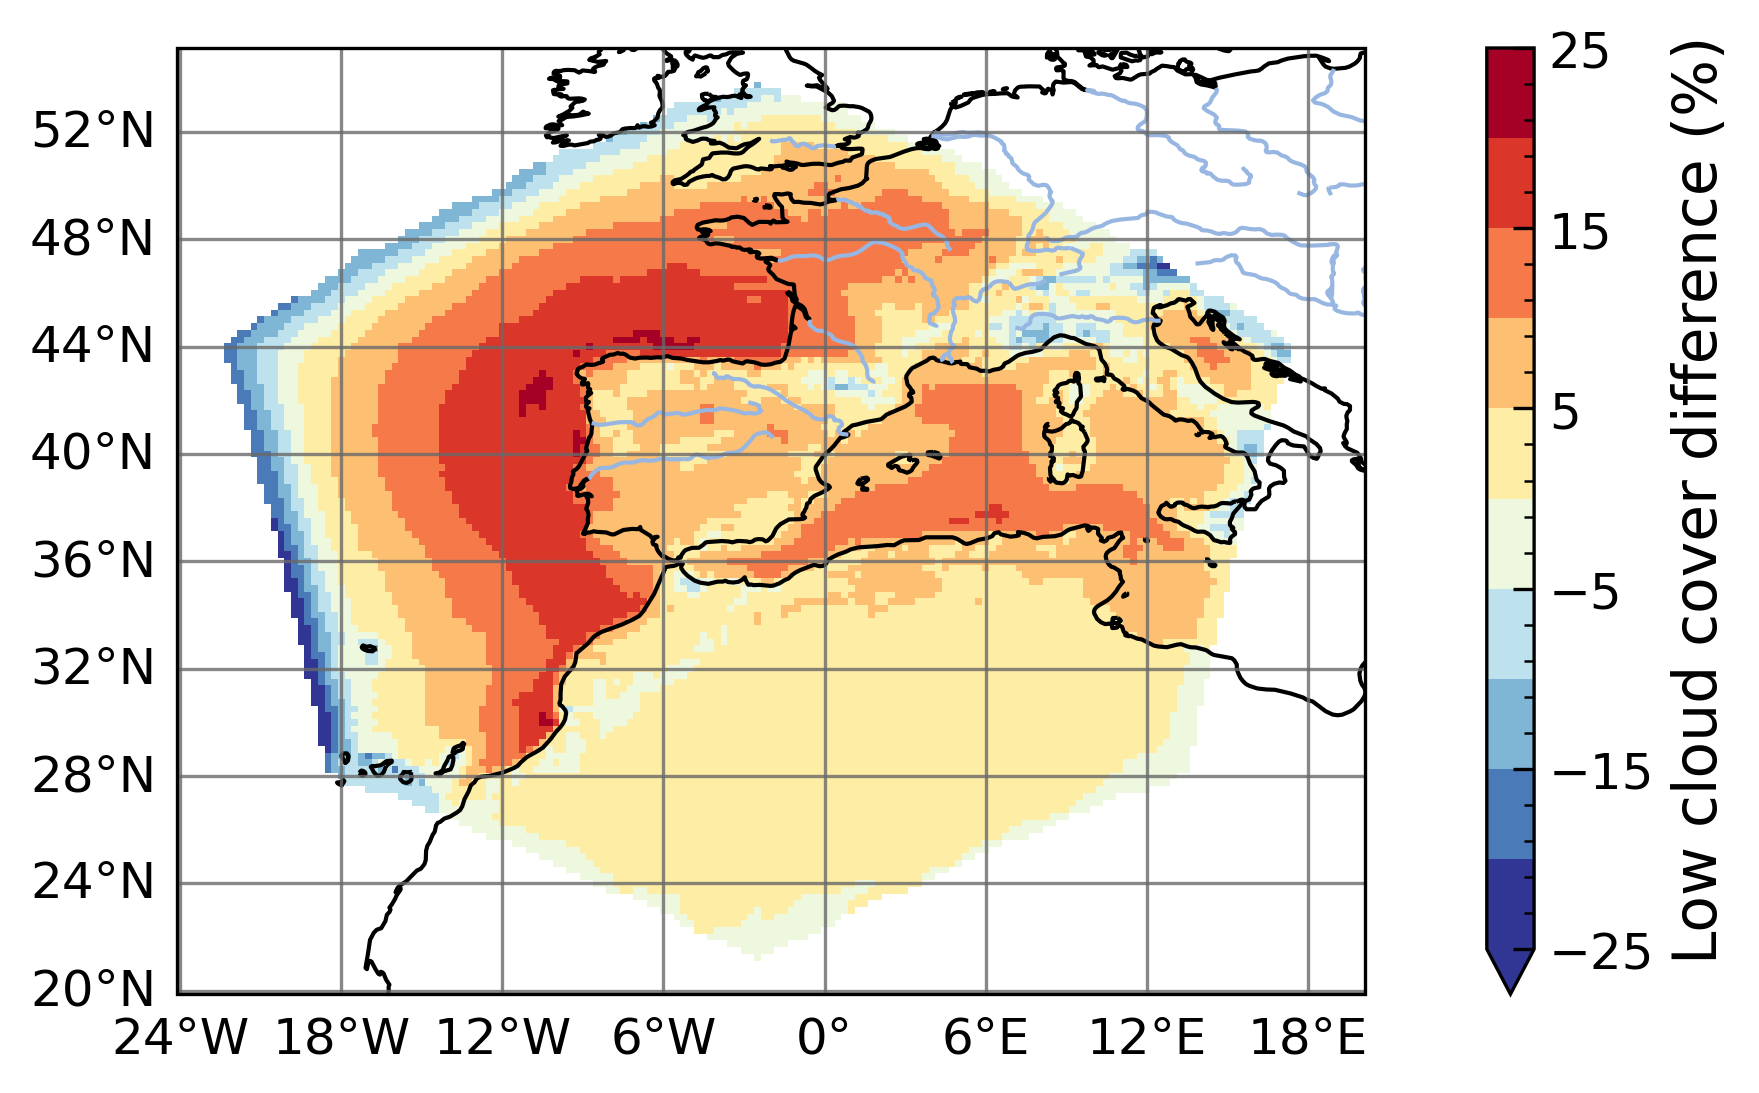
\includegraphics[width=\textwidth]{images/chap4/domain_size/diff_map_cldl_era_LAM_2000km_NBP80.png}
        \end{subfigure} \\

        %SWdn
        \begin{subfigure}[b]{0.33\textwidth}
            \caption{Downwelling SW flux bias\\(W \persqm, \smalld)}
            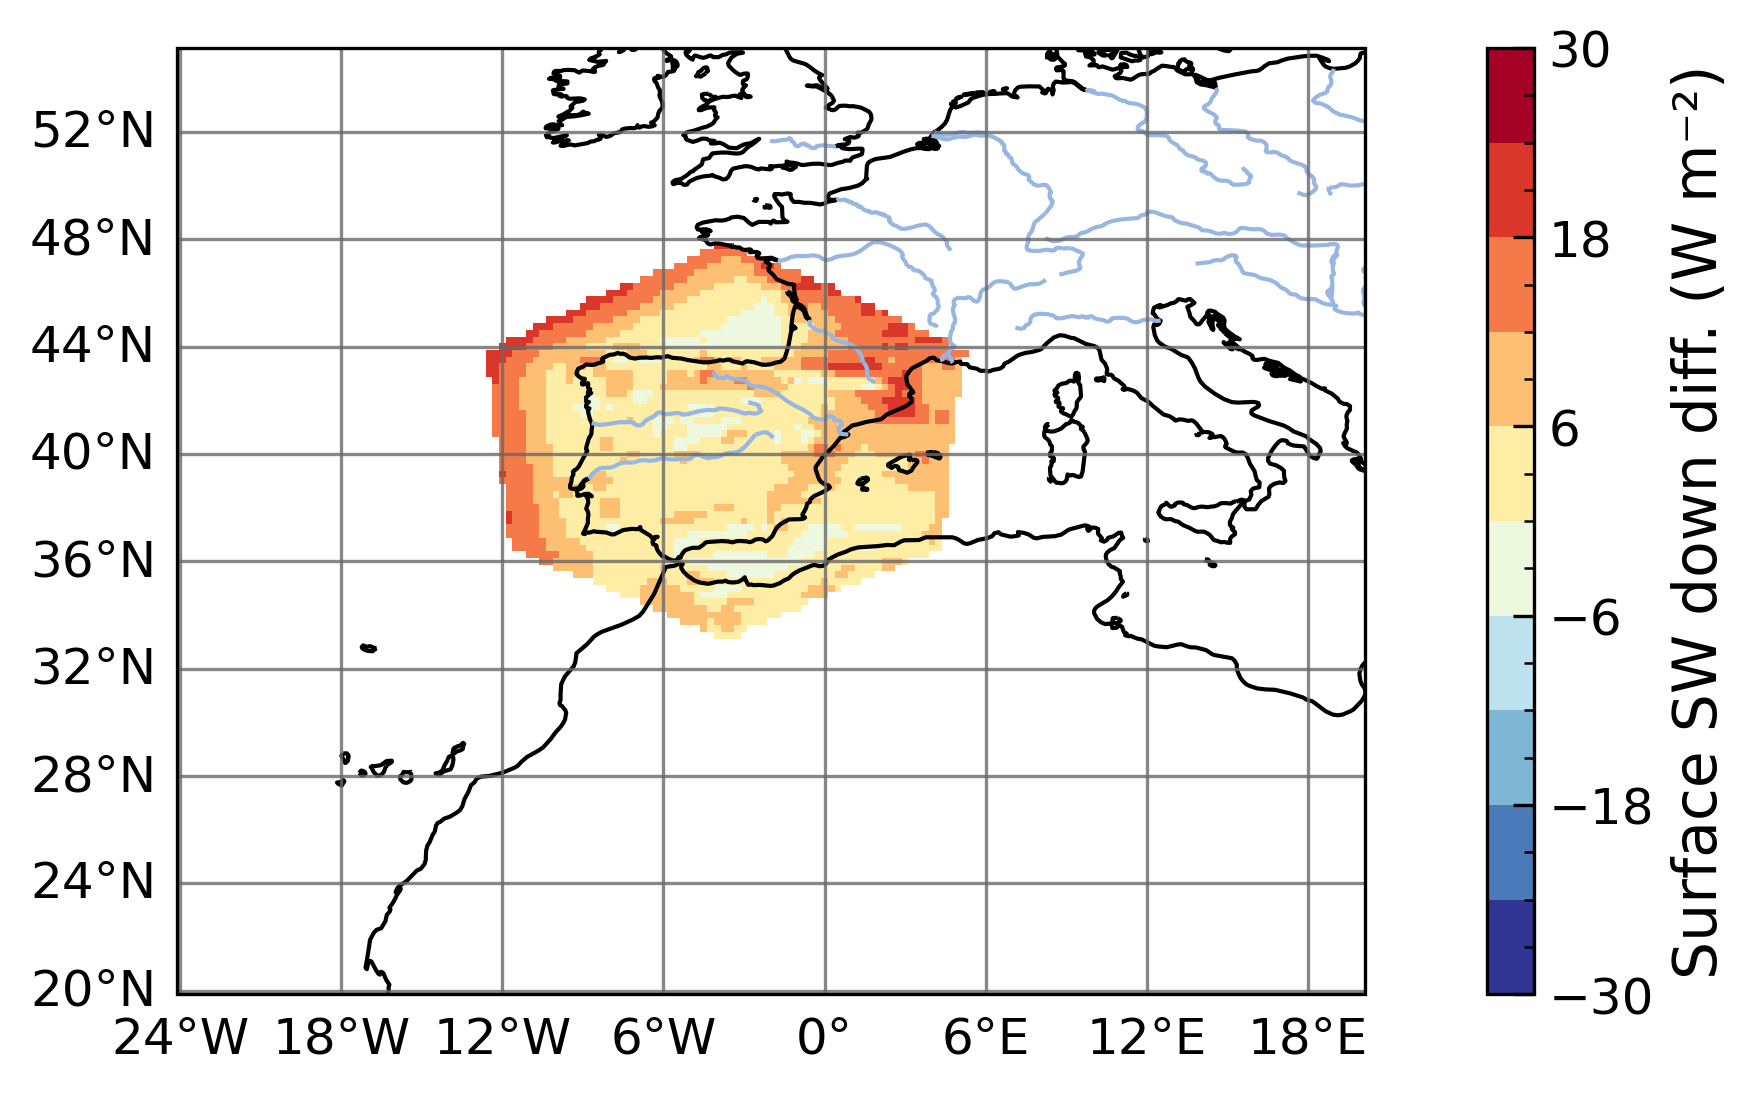
\includegraphics[width=\textwidth]{images/chap4/domain_size/diff_map_SWdnSFC_era_LAM_1000km_NBP40.png}
        \end{subfigure} &
        \begin{subfigure}[b]{0.33\textwidth}
            \caption{Downwelling SW flux bias\\(W \persqm, \interd)}
            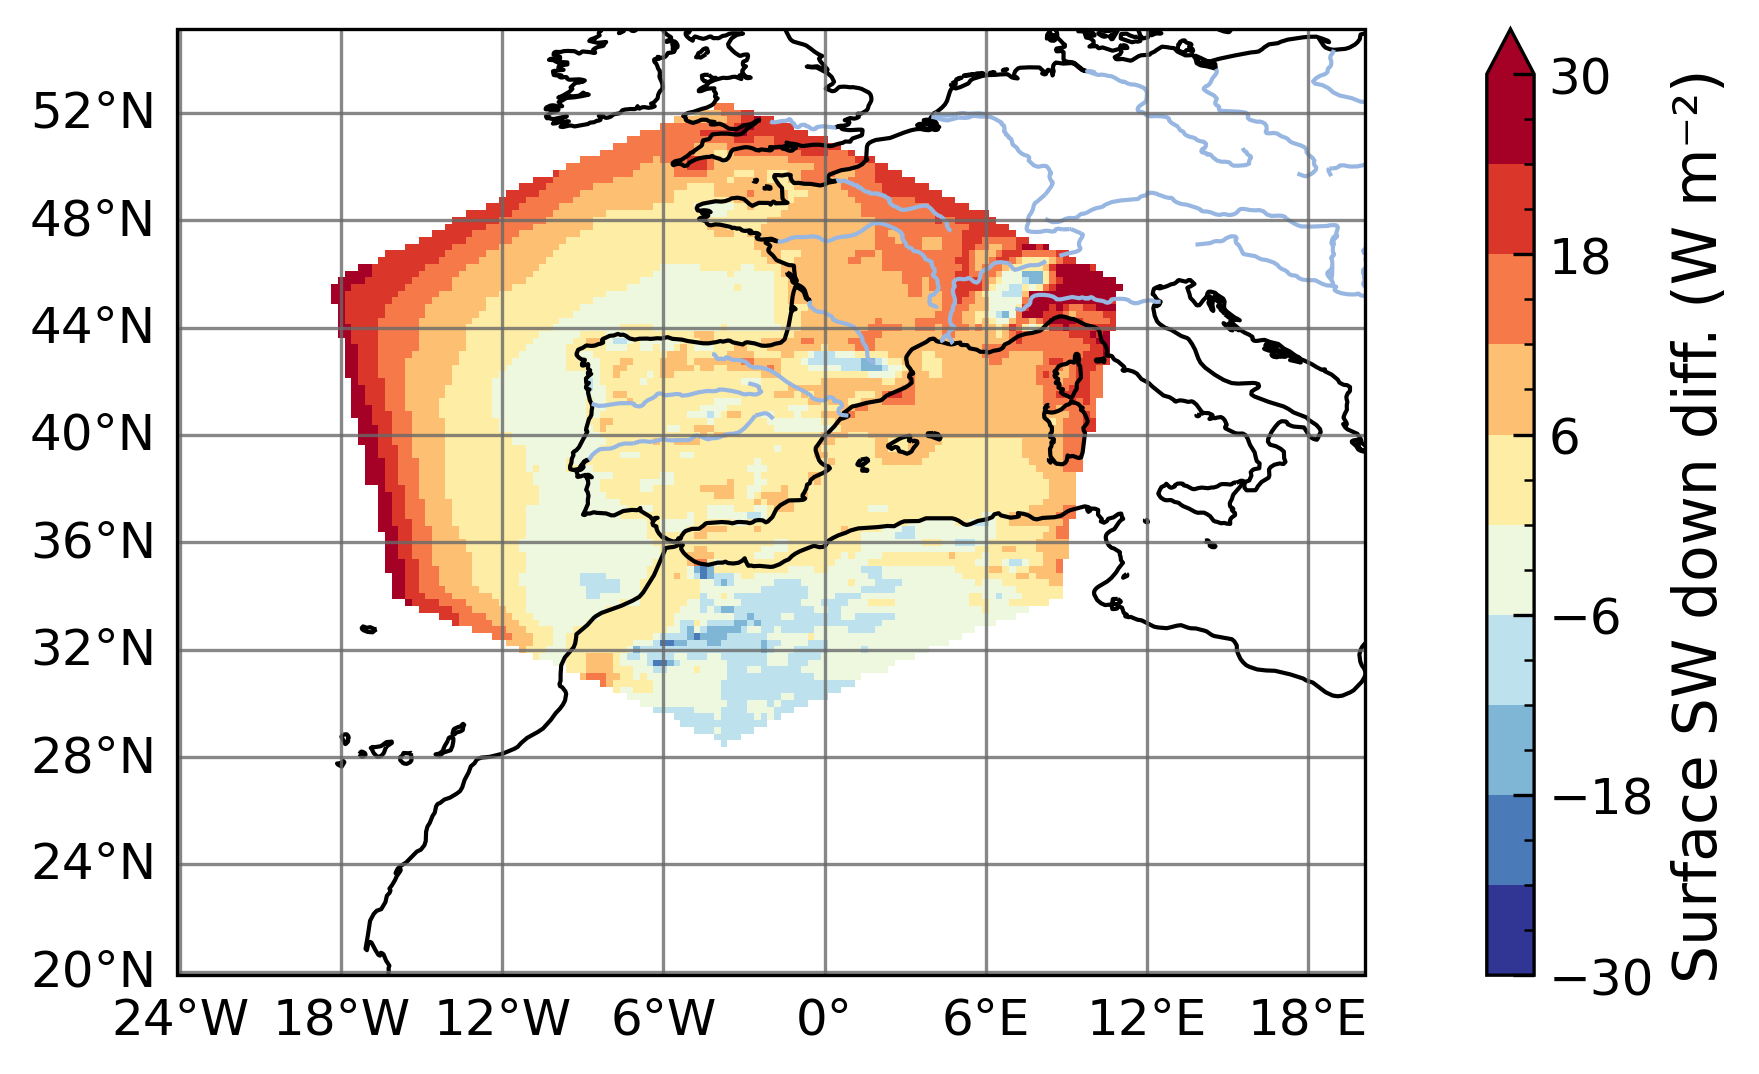
\includegraphics[width=\textwidth]{images/chap4/domain_size/diff_map_SWdnSFC_era_LAM_1500km_NBP60.png}
        \end{subfigure} &
        \begin{subfigure}[b]{0.33\textwidth}
            \caption{Downwelling SW flux bias\\(W \persqm, \larged)}
            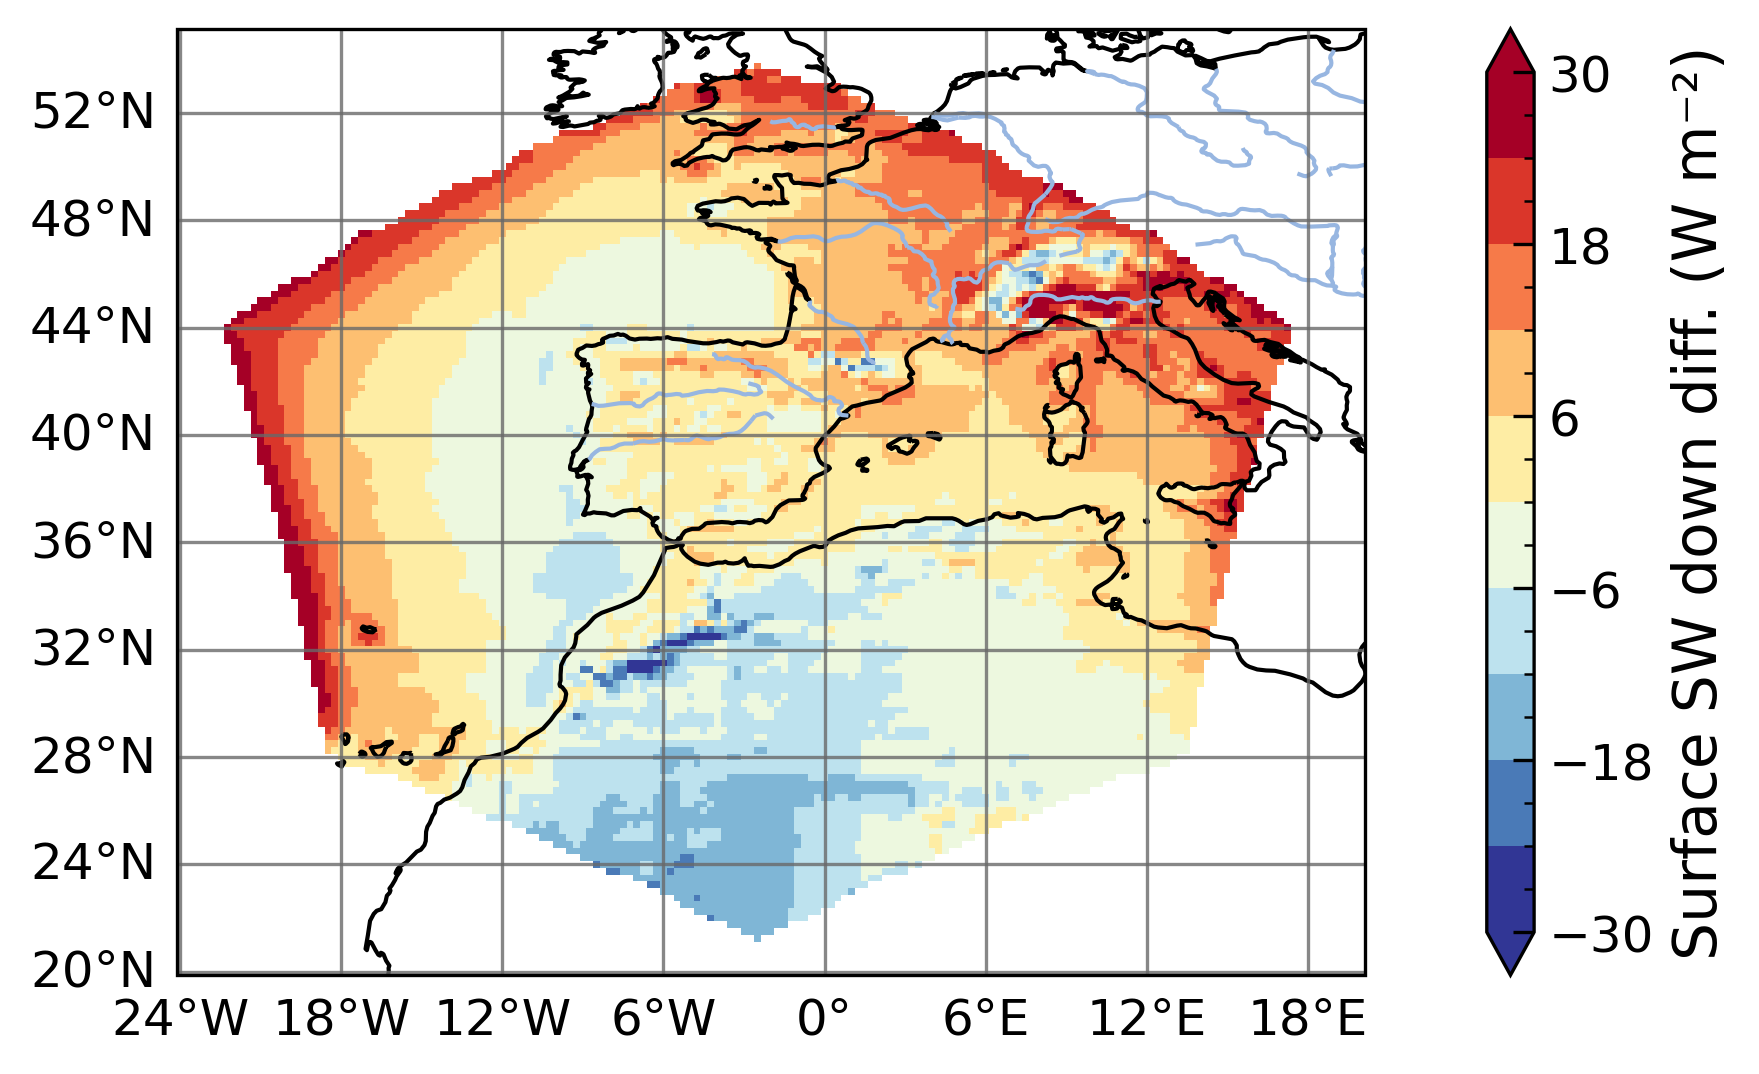
\includegraphics[width=\textwidth]{images/chap4/domain_size/diff_map_SWdnSFC_era_LAM_2000km_NBP80.png}
        \end{subfigure} \\
        
        %LWdn
        \begin{subfigure}[b]{0.33\textwidth}
            \caption{Downwelling LW flux bias\\(W \persqm, \smalld)}
            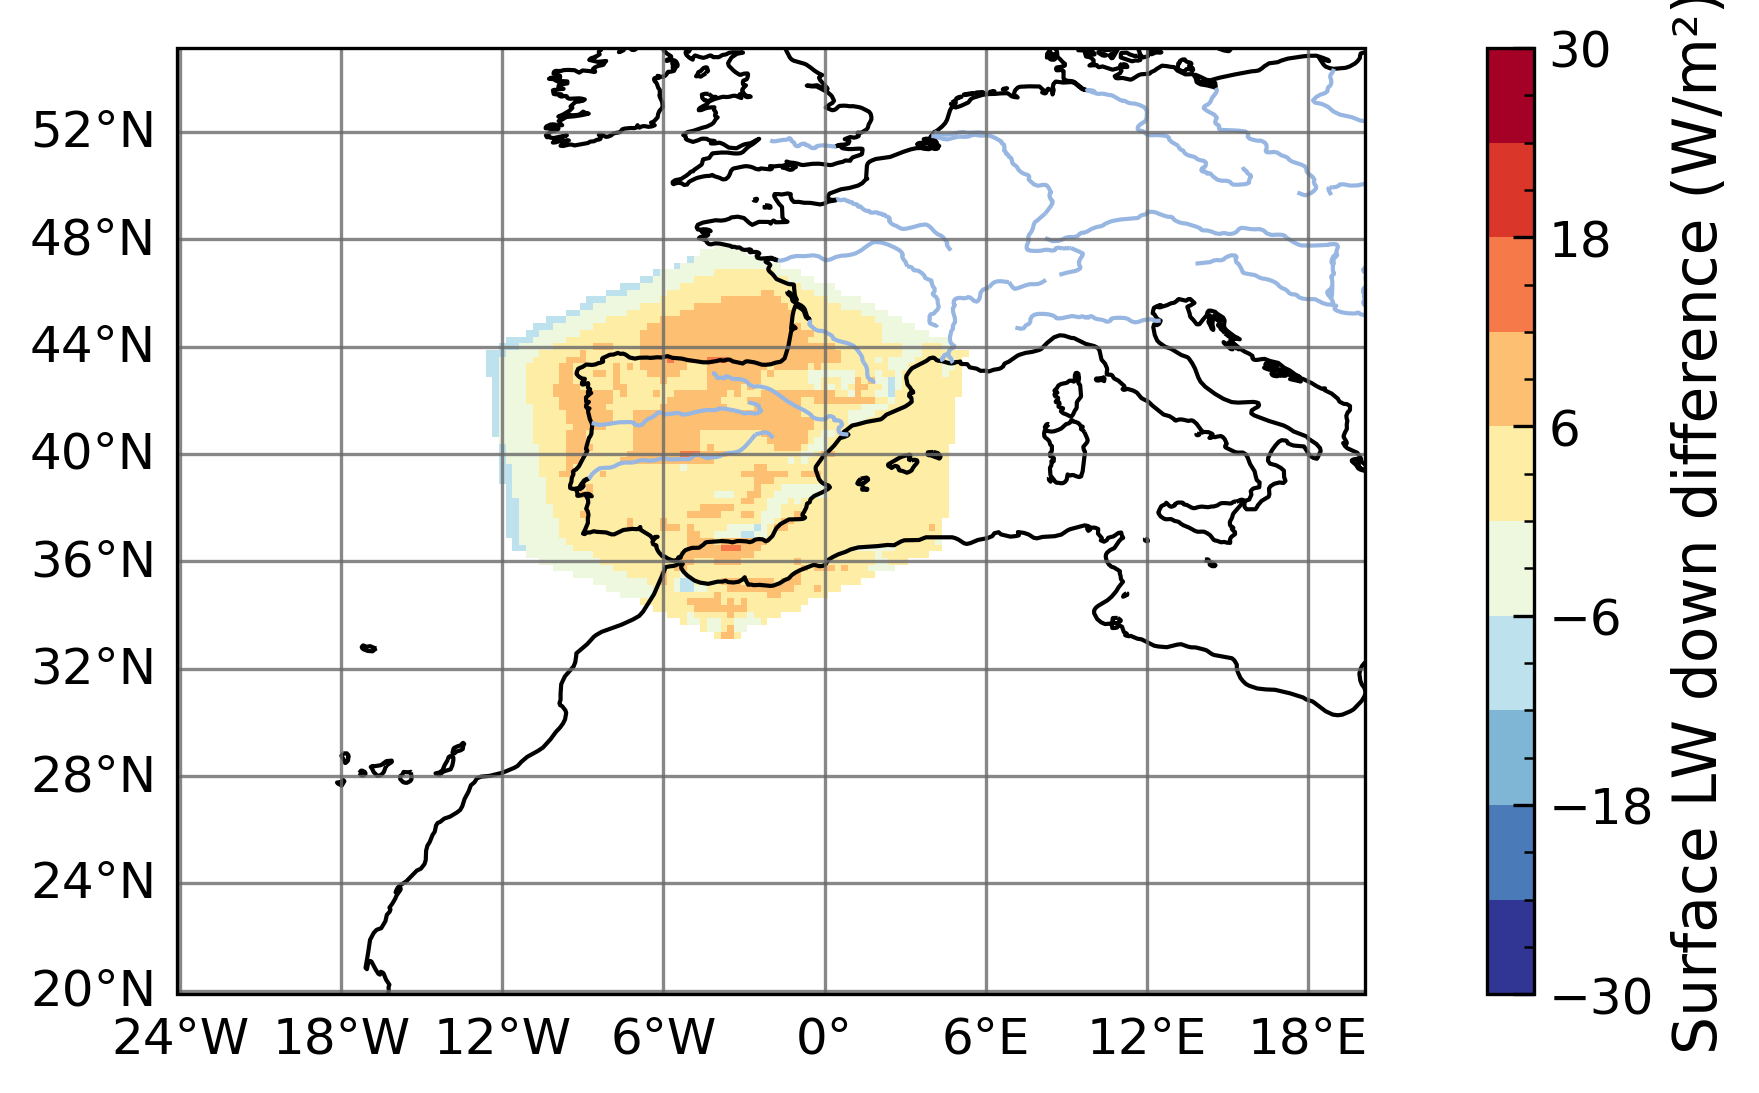
\includegraphics[width=\textwidth]{images/chap4/domain_size/diff_map_LWdnSFC_era_LAM_1000km_NBP40.png}
        \end{subfigure} &
        \begin{subfigure}[b]{0.33\textwidth}
            \caption{Downwelling LW flux bias\\(W \persqm, \interd)}
            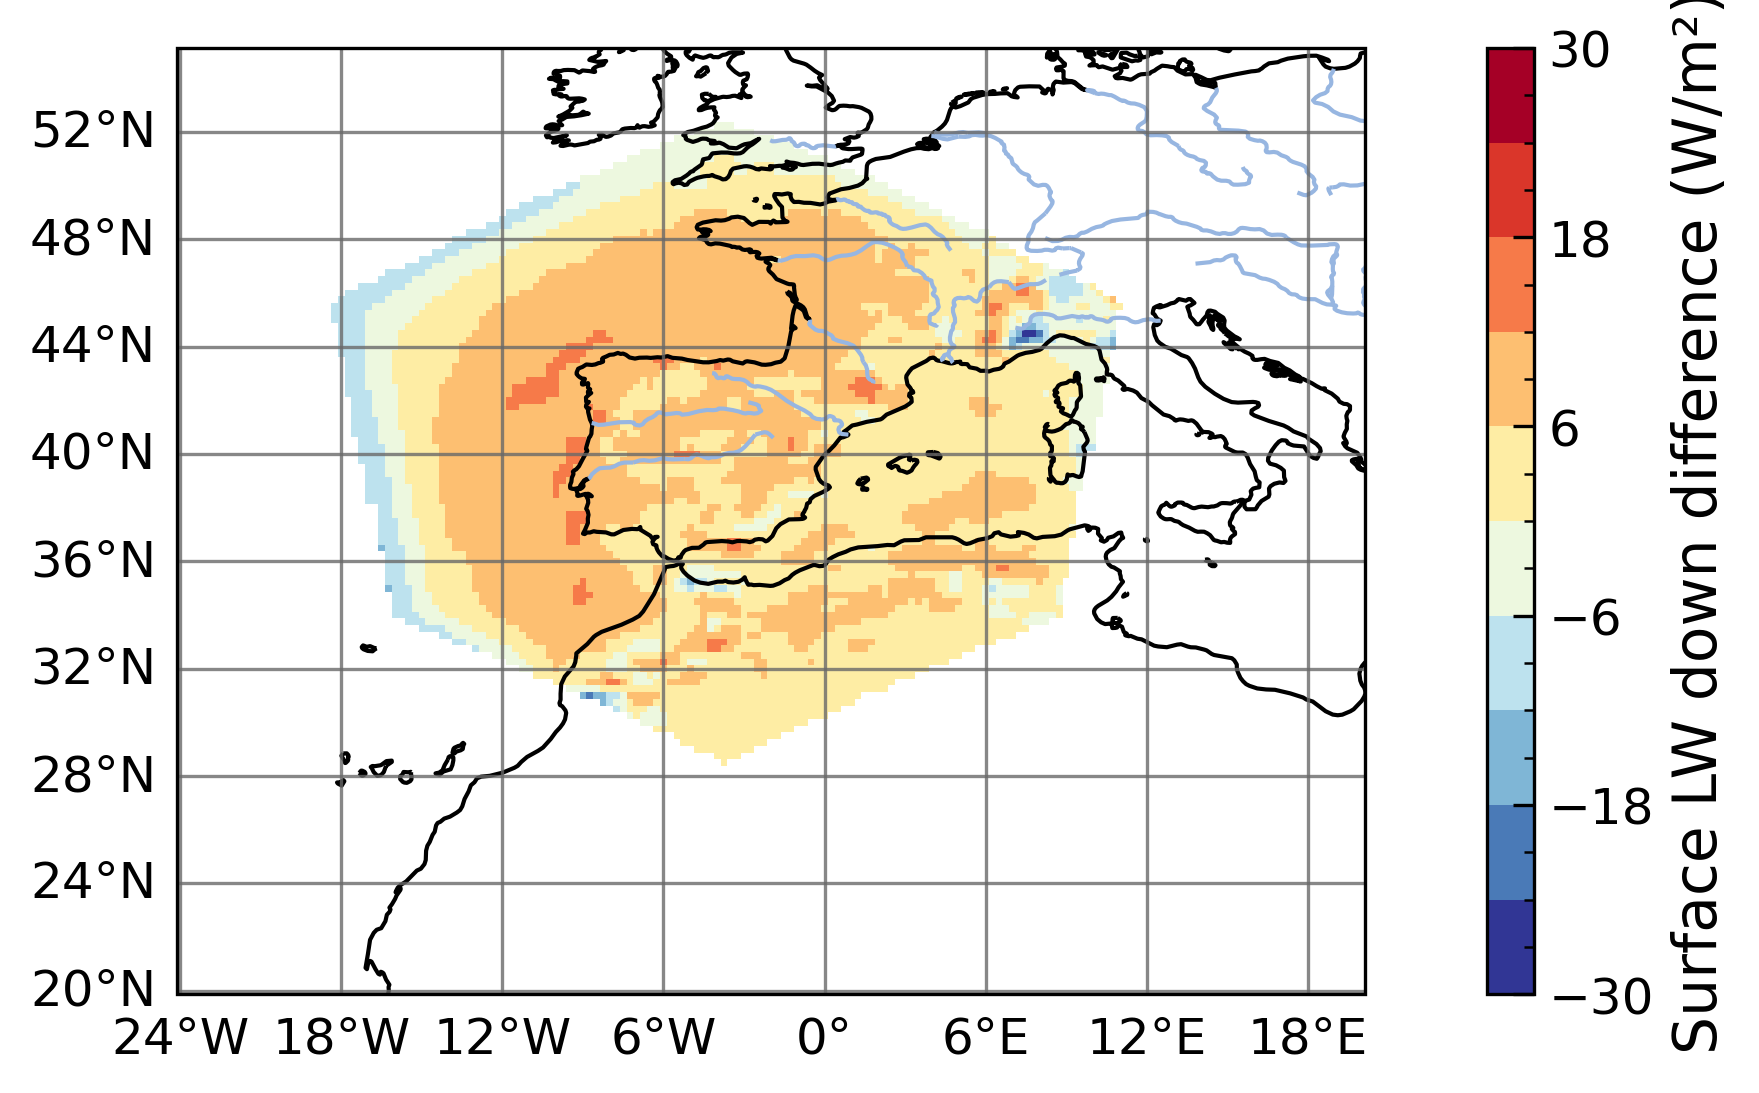
\includegraphics[width=\textwidth]{images/chap4/domain_size/diff_map_LWdnSFC_era_LAM_1500km_NBP60.png}
        \end{subfigure} &
        \begin{subfigure}[b]{0.33\textwidth}
            \caption{Downwelling LW flux bias\\(W \persqm, \larged)}
            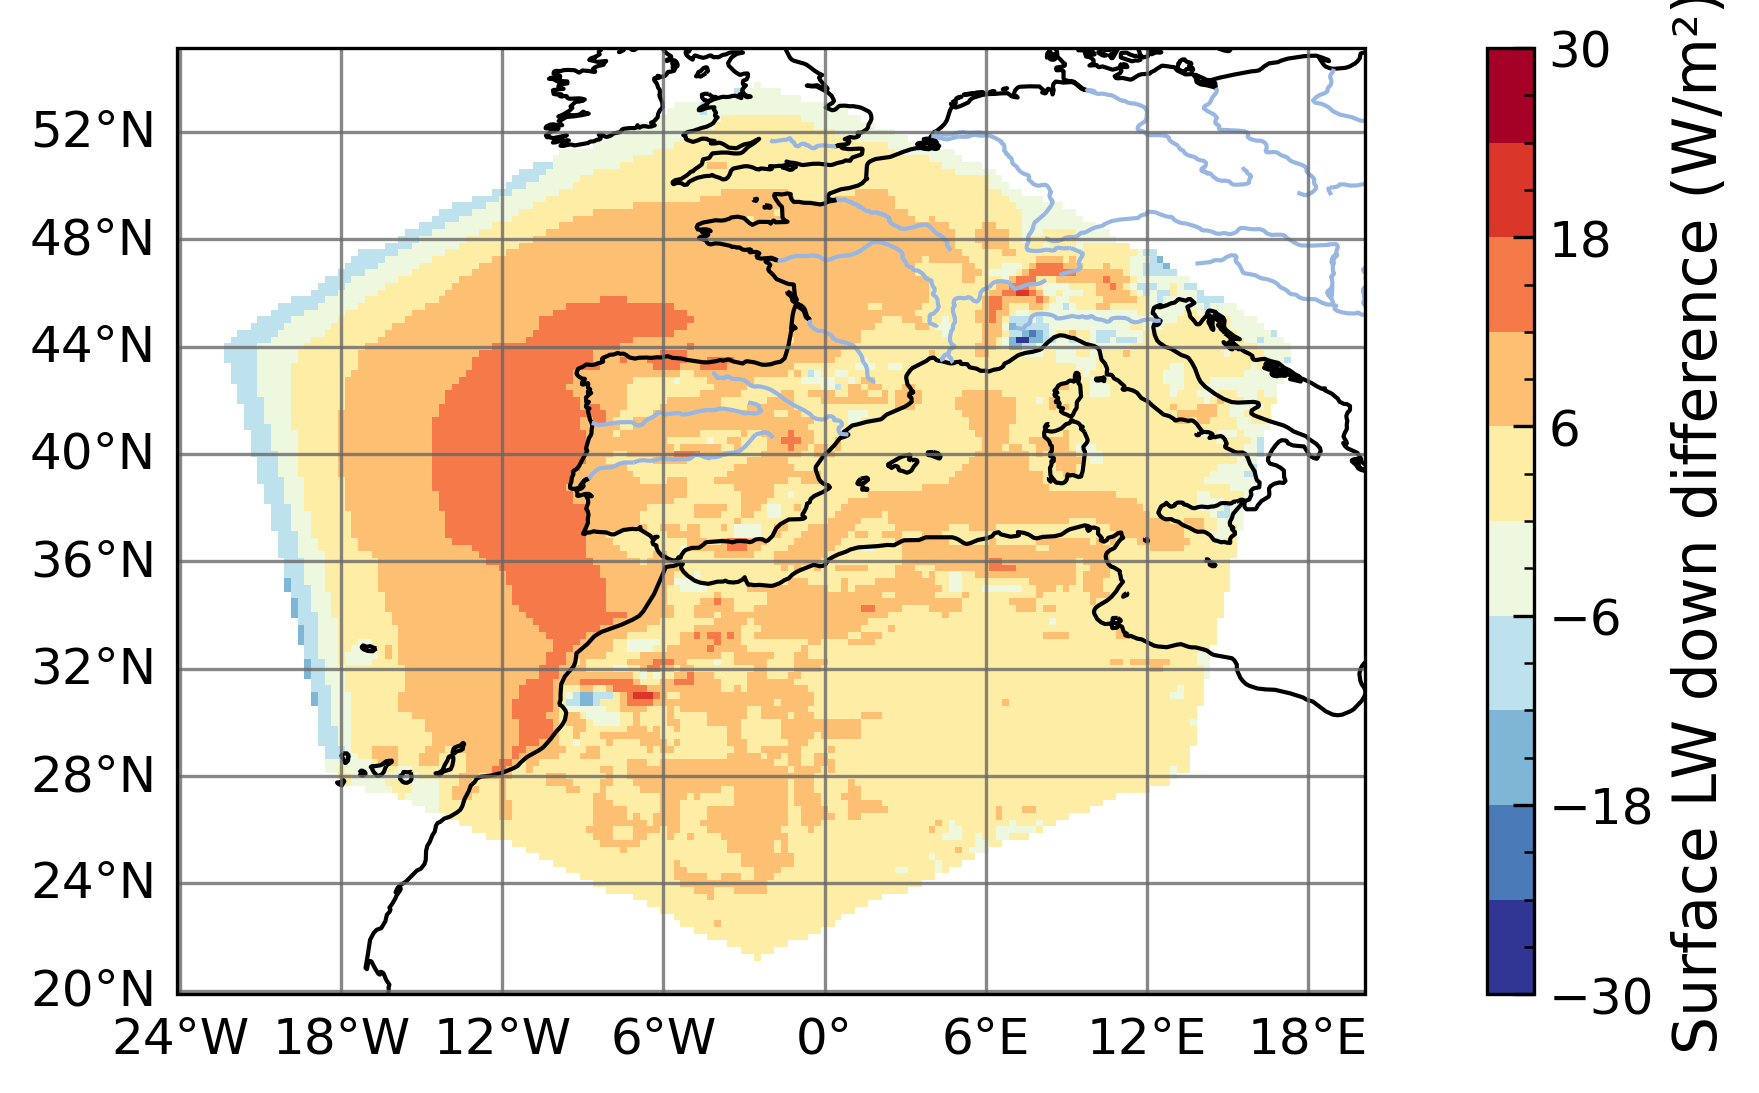
\includegraphics[width=\textwidth]{images/chap4/domain_size/diff_map_LWdnSFC_era_LAM_2000km_NBP80.png}
        \end{subfigure}
    \end{tabular}
    \caption{Cloud cover and downwelling radiative fluxes biases to ERA5 over 2010-2014 for three simulations with small, intermediate and large domain sizes.}
    \label{fig:domain_size_clouds_ERA_diff_maps}
\end{figure}

These results confirmed the hypothesis that the LAM is not able to condense water normally in the transition zone where it is nudged towards the forcing data from the ERA5 reanalysis. This was attributed to the fact that the ERA5 data is obtained with a model that has its own physics scheme, possibly functionning very differently from the LMDZ physics, and that the continuous nudging does not give the physics of the LAM the freedom it needs to condense water. This would explain the low values of cloud cover and the very low precipitation in this zone.

In the free zone of the LAM, the model once again behaves normally, but can partly be influenced by the transition zone through the dynamics, meaning that the influence of the forcing and of the discrepancies between the physics of ERA5 and ICOLMDZ is not strictly confined to the transition zone.
This analysis and the comparison of three domain sizes showed that in \smalld, the underestimation of precipitation is impacting some parts of the Peninsula, and that biases in ET are not limited to the edges but extended to the coast of the study area. With the two larger domains, although some biases persist over the Peninsula, their structure does not seem to be the consequence of the discrepancies in the transition zone. Clear progress in the consistency of the LAM was obtained by changing from the small to the intermediate domain, but as there was no obvious improvements between the intermediate and large domain, the \interd simulation setup with $R_{domain} = 1500 km$ and $NBP = 60$ was used for the rest of the study (results presented in Section \ref{sec:article1} and Chapter \ref{chap:liaise}).

Meanwhile,  to explore the hypothesis that the biases in the transition zone are due to discrepancies between the physics of ICOLMDZ and ERA5, LAM simulations using the small domain were run using a global ICOLMDZOR simulation as the source for the forcing file. The results of this analysis are presented in the following Section \ref{sec:forcing_source}.

\clearpage

\section{Impact of the source of the lateral forcing}
\label{sec:forcing_source}

%figure : maps of diff vs ERA for 2 forcing sources
\begin{figure}[!h]
    \centering
    \begin{tabular}{cc}
        %precip
        \begin{subfigure}[b]{0.33\textwidth}
            \caption{Precipitation bias\\(mm \perday, \forcingERA)}
            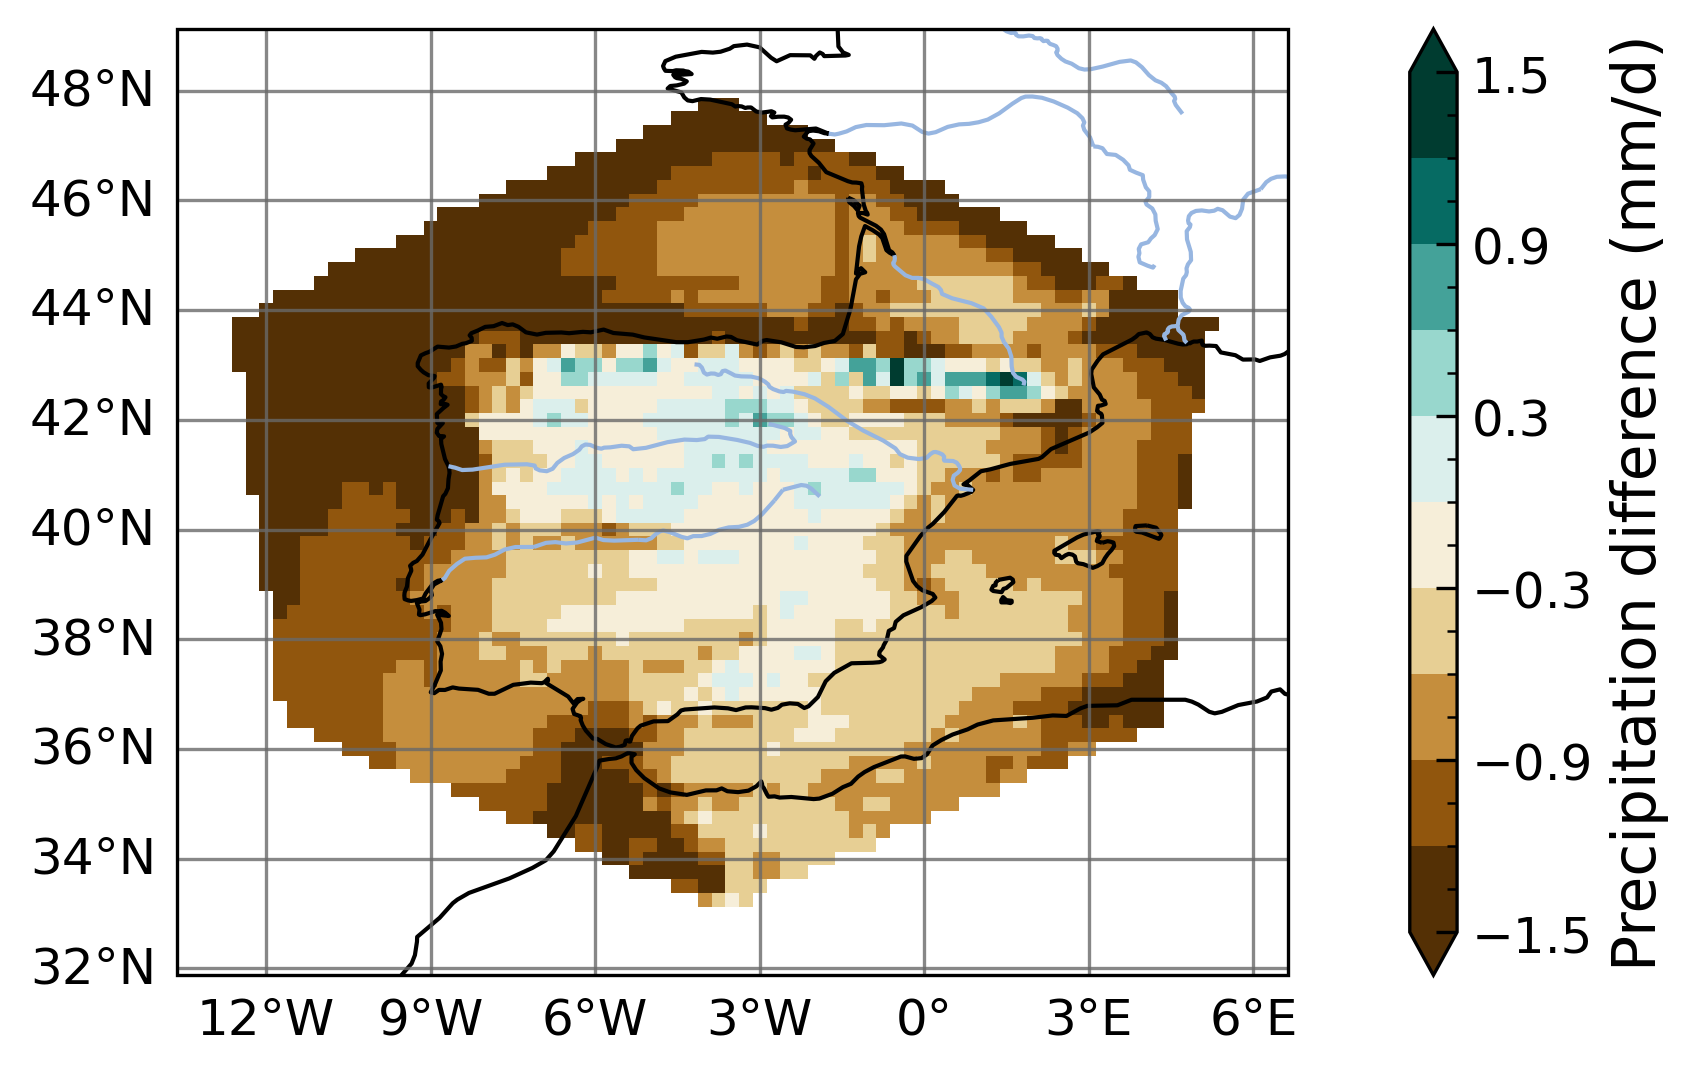
\includegraphics[width=\textwidth]{images/chap4/forcing_source/diff_map_precip_era_era.png}
        \end{subfigure} &
        \begin{subfigure}[b]{0.33\textwidth}
            \caption{Precipitation bias\\(mm \perday, \forcingICO)}
            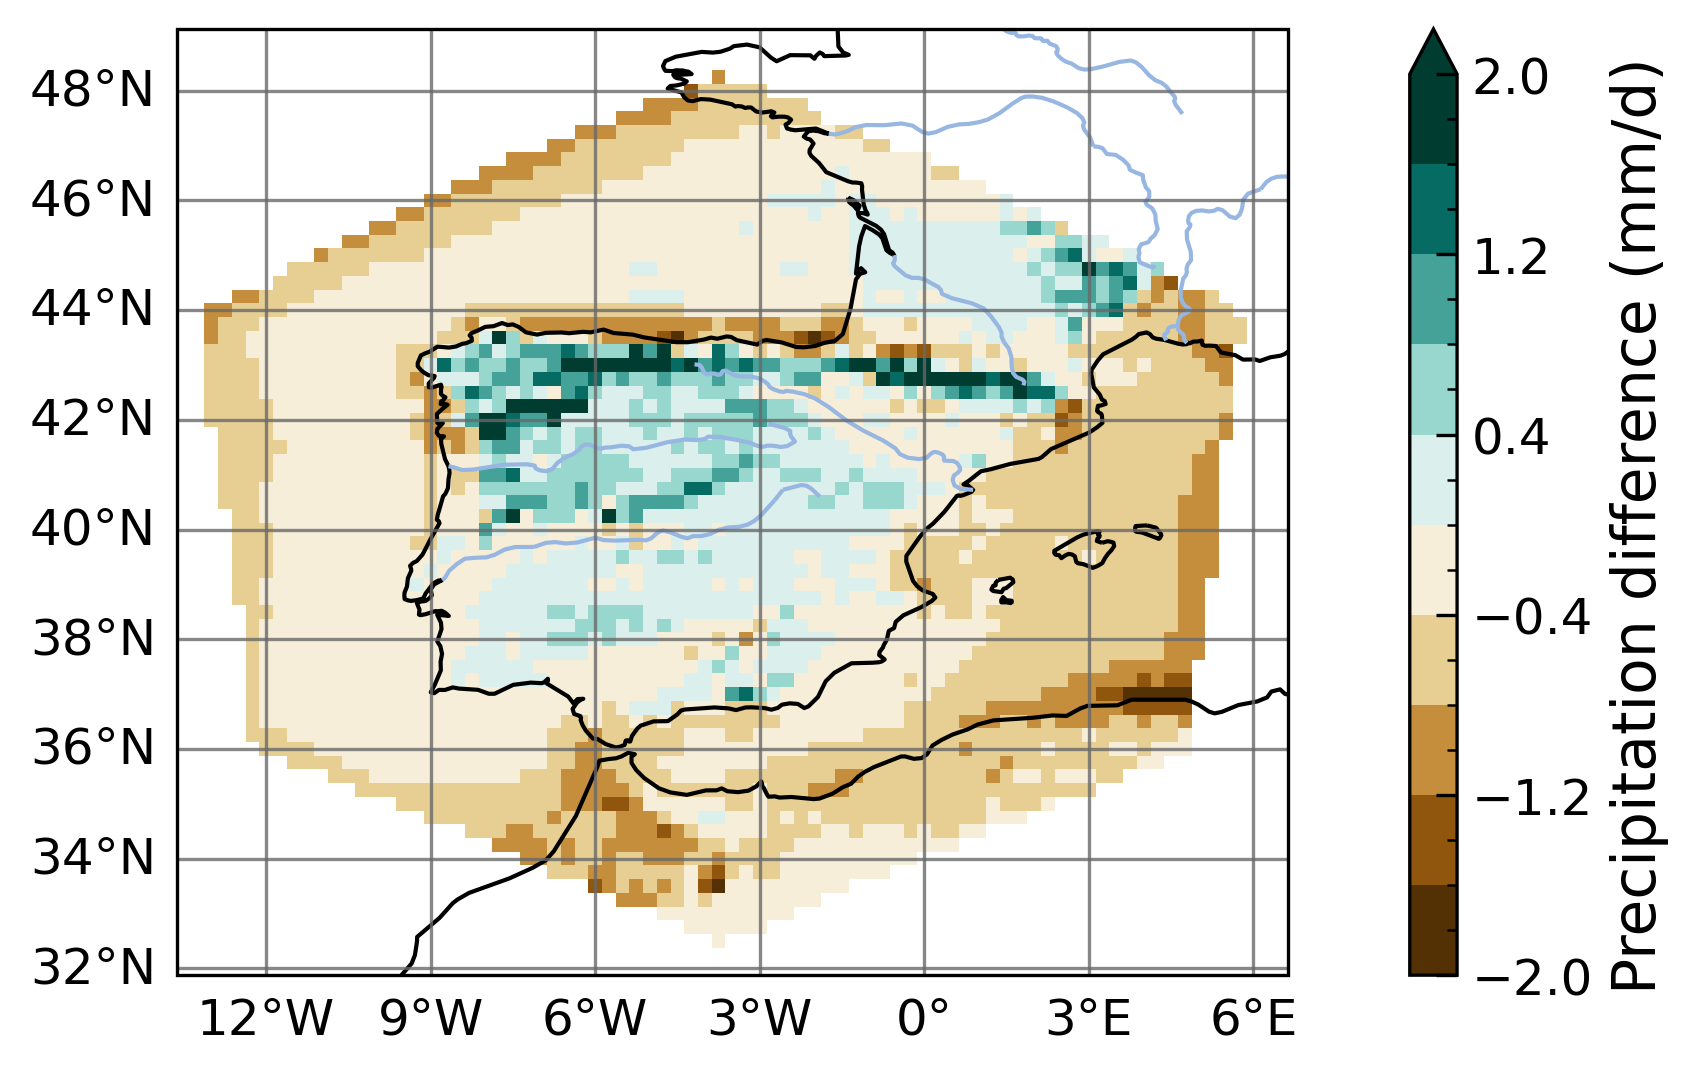
\includegraphics[width=\textwidth]{images/chap4/forcing_source/diff_map_precip_ico_era.png}
        \end{subfigure} \\
        %evap
        \begin{subfigure}[b]{0.33\textwidth}
            \caption{ET bias\\(mm \perday, \forcingERA)}
            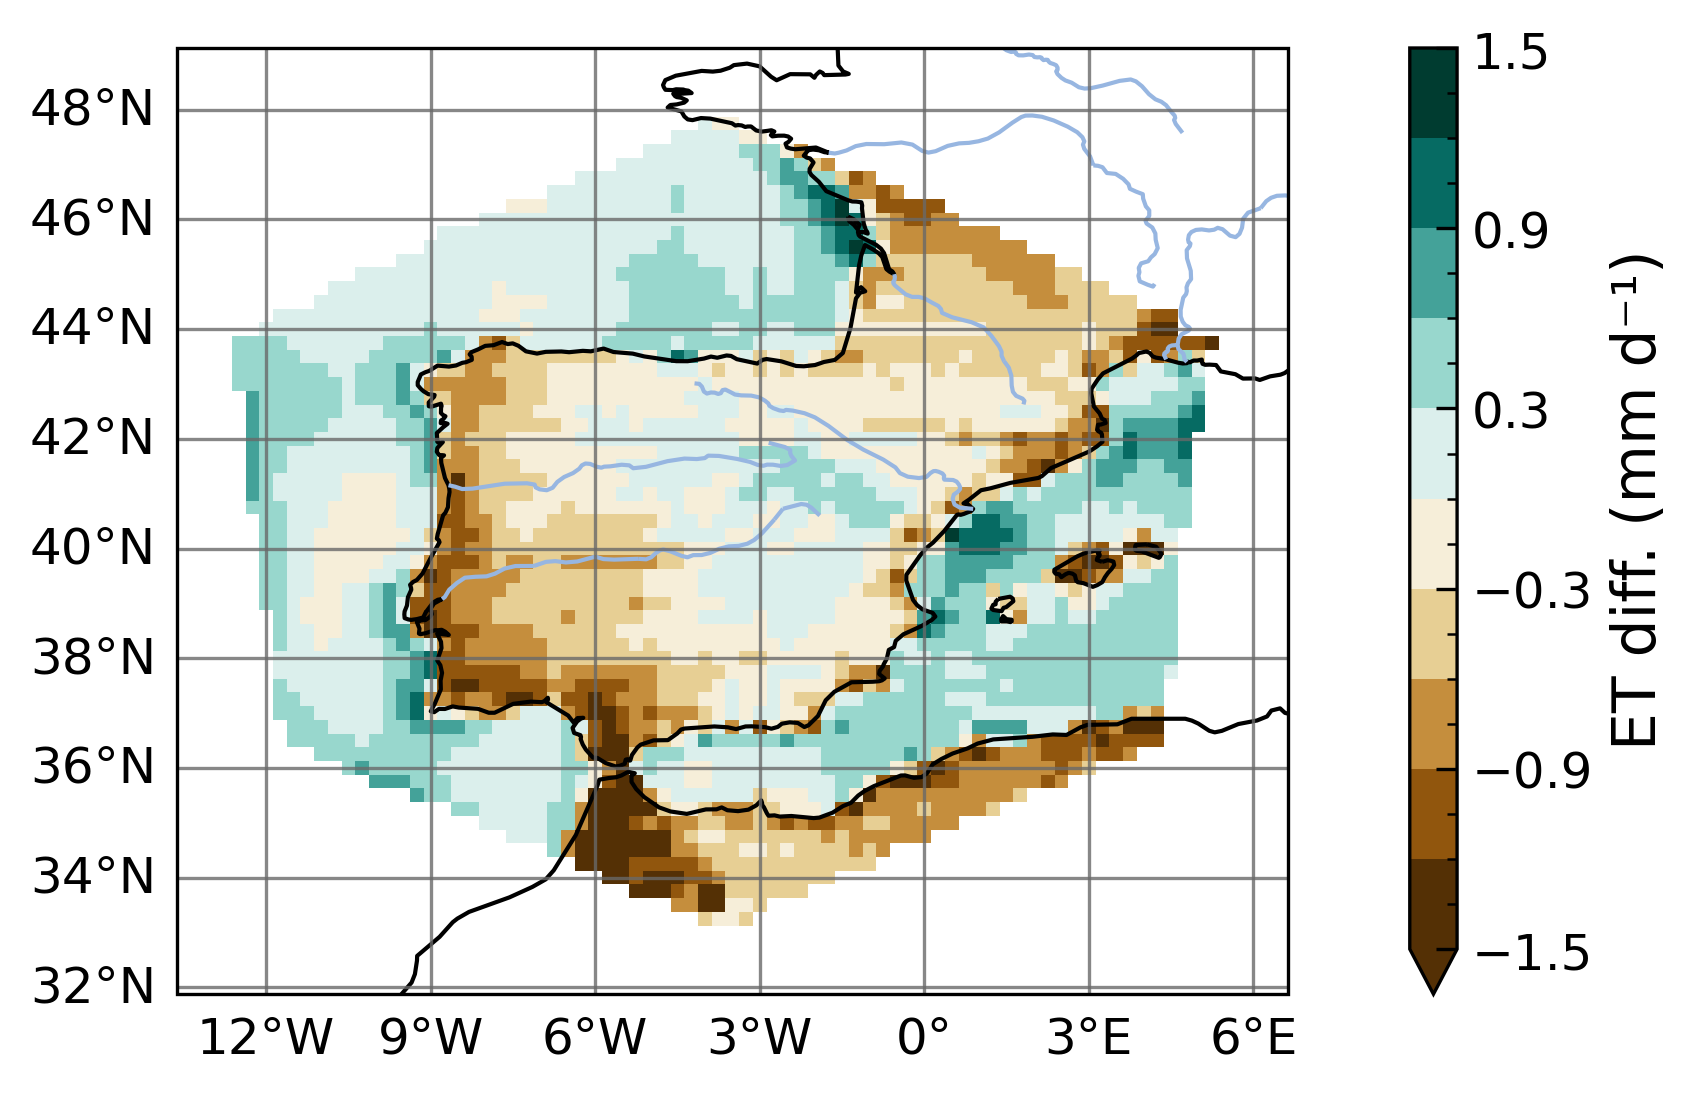
\includegraphics[width=\textwidth]{images/chap4/forcing_source/diff_map_evap_era_era.png}
        \end{subfigure} &
        \begin{subfigure}[b]{0.33\textwidth}
            \caption{ET bias\\(mm \perday, \forcingICO)}
            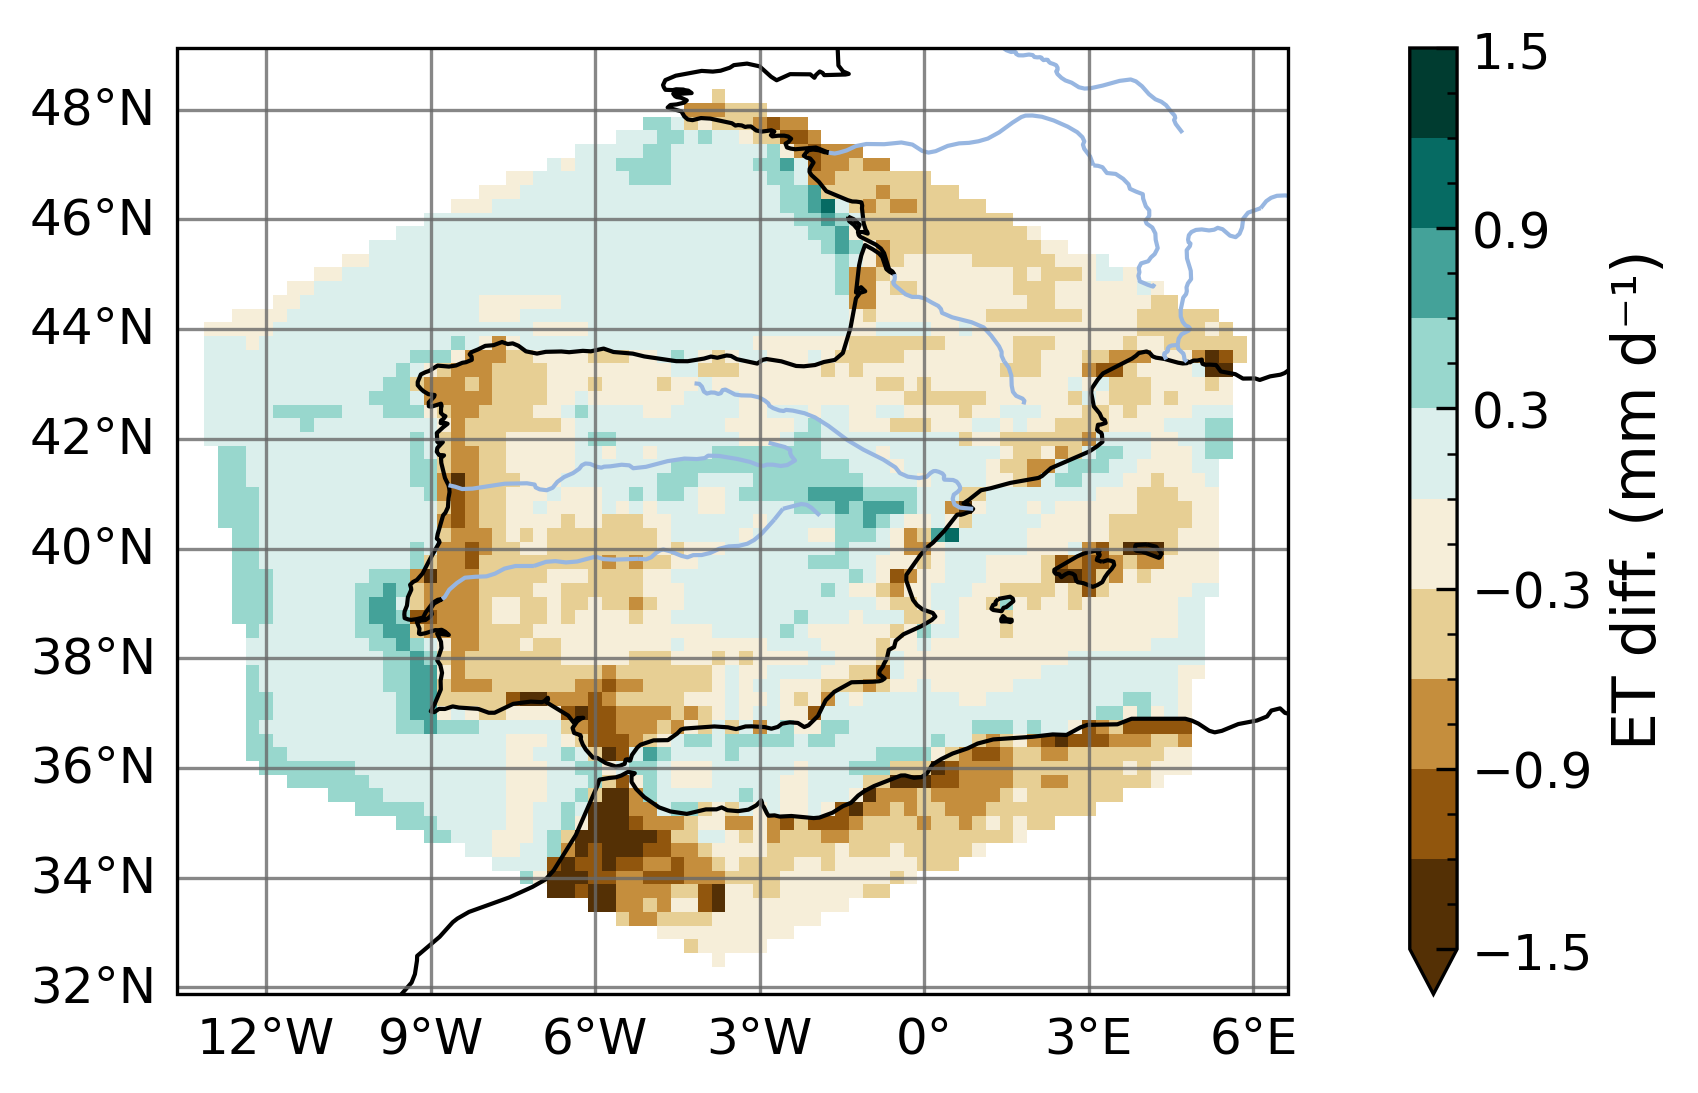
\includegraphics[width=\textwidth]{images/chap4/forcing_source/diff_map_evap_ico_era.png}
        \end{subfigure} \\
        %SWdn
        \begin{subfigure}[b]{0.33\textwidth}
            \caption{Downwelling SW flux bias\\(W \persqm, \forcingERA)}
            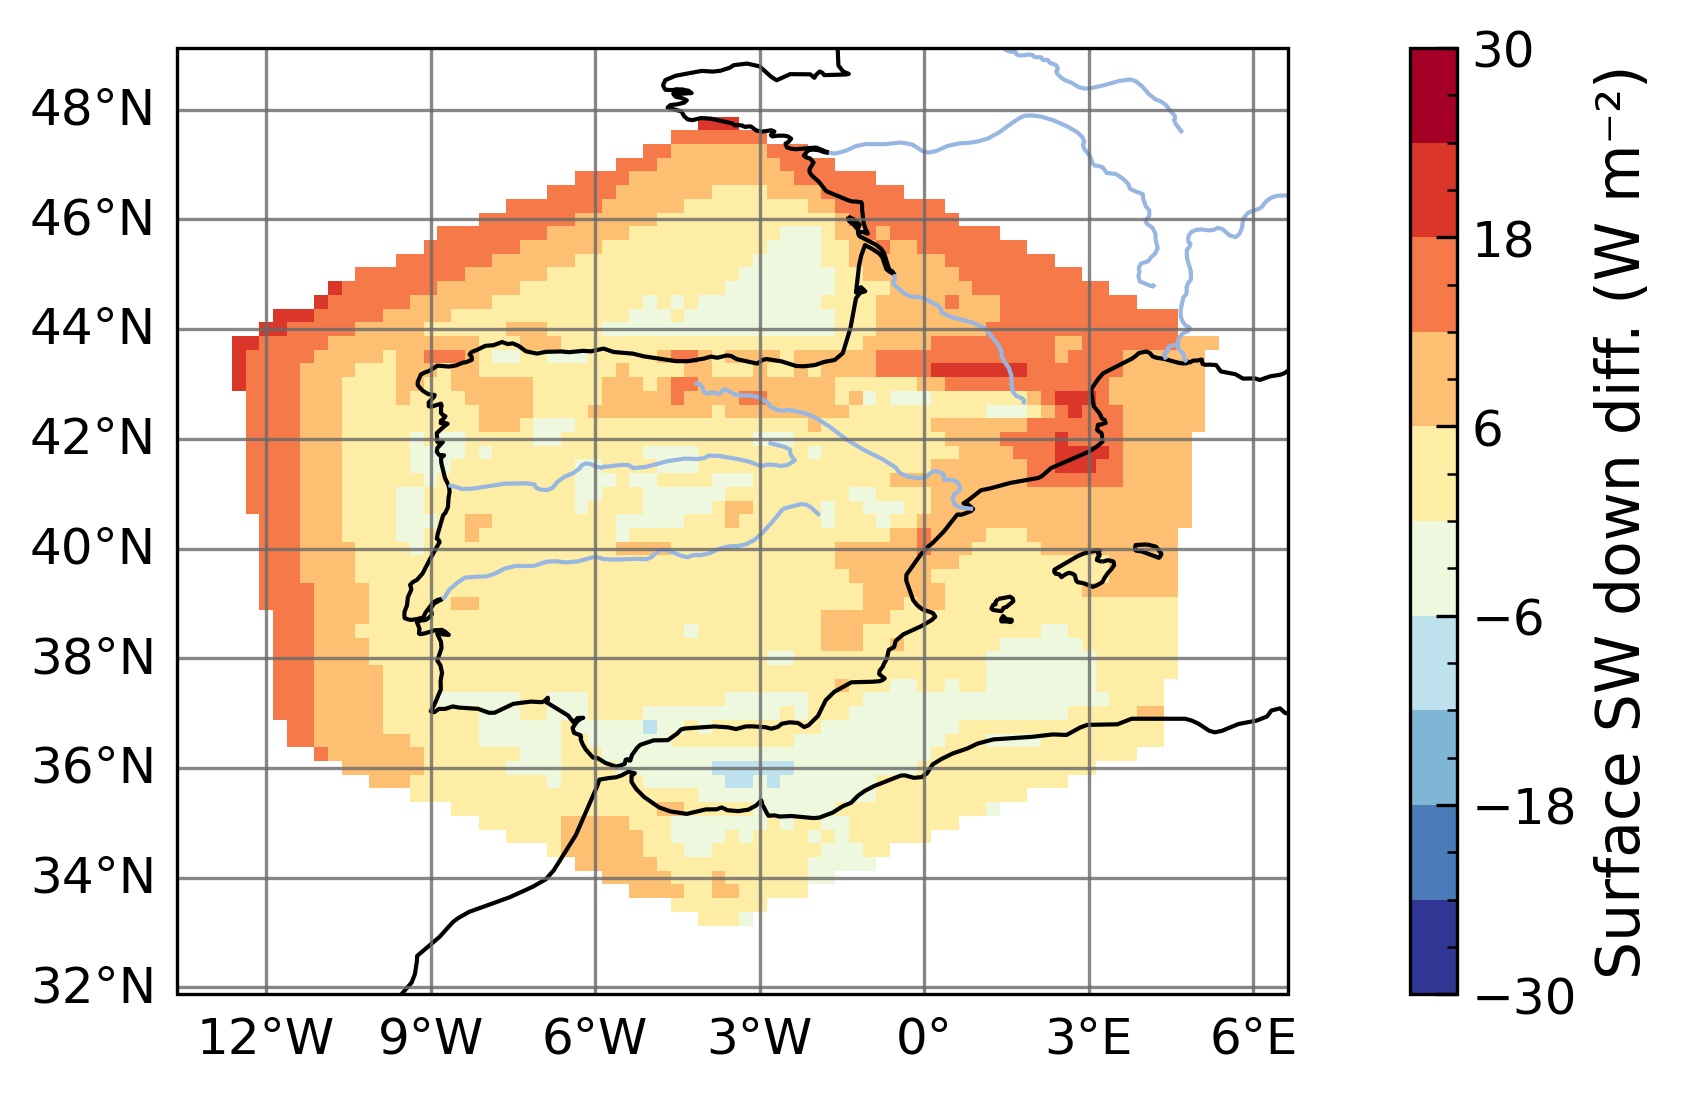
\includegraphics[width=\textwidth]{images/chap4/forcing_source/diff_map_SWdnSFC_era_era.png}
        \end{subfigure} &
        \begin{subfigure}[b]{0.33\textwidth}
            \caption{Downwelling SW flux bias\\(W \persqm, \forcingICO)}
            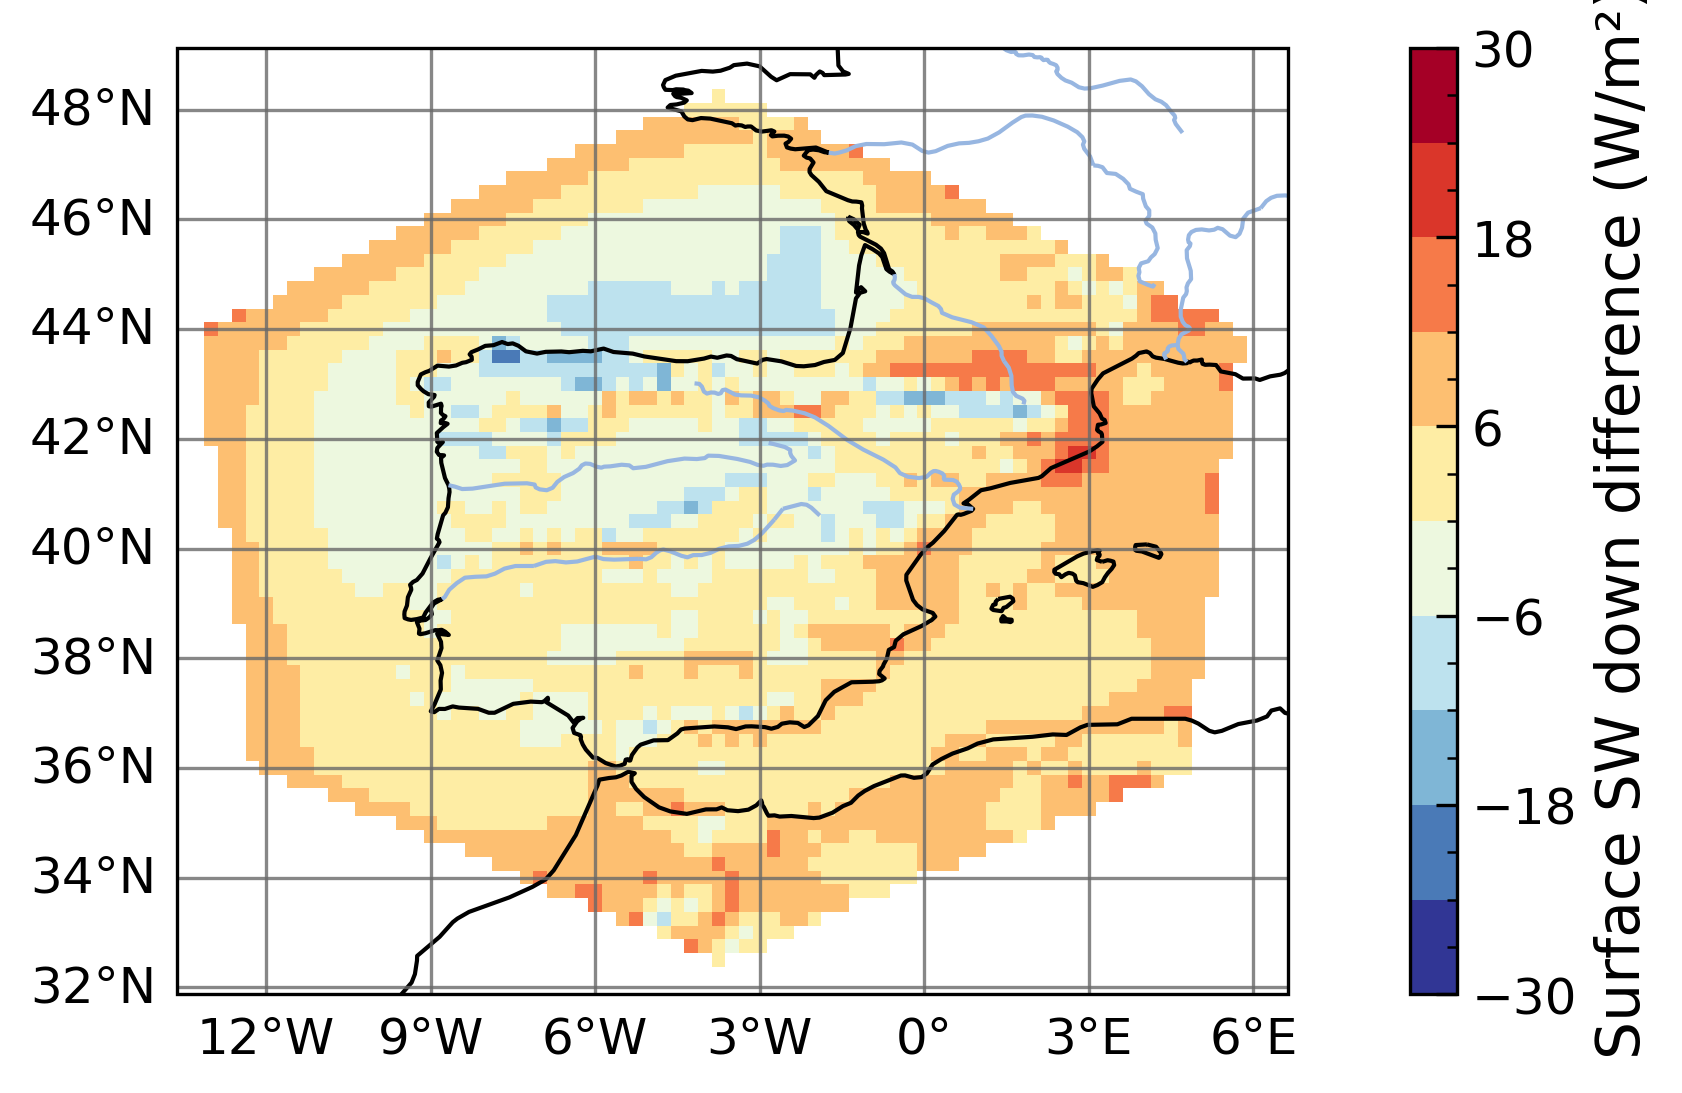
\includegraphics[width=\textwidth]{images/chap4/forcing_source/diff_map_SWdnSFC_ico_era.png}
        \end{subfigure}\\
        %LWdn
        \begin{subfigure}[b]{0.33\textwidth}
            \caption{Downwelling LW flux bias\\(W \persqm, \forcingERA)}
            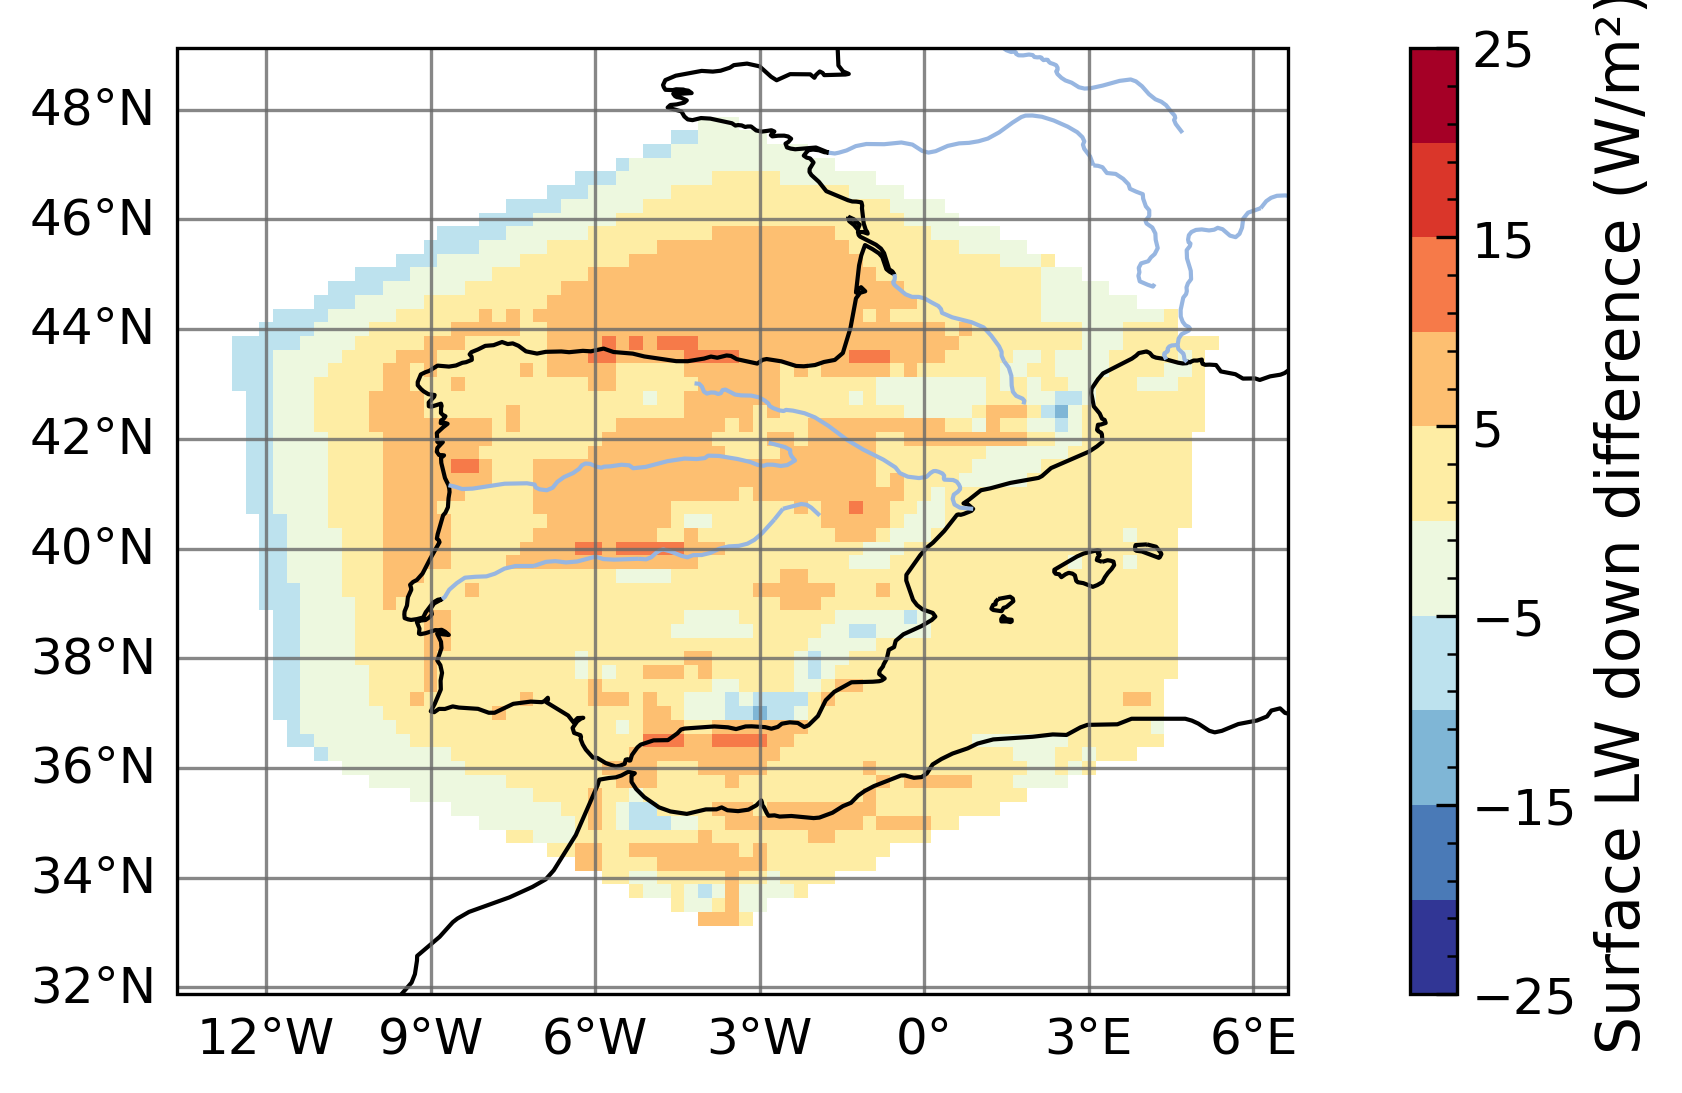
\includegraphics[width=\textwidth]{images/chap4/forcing_source/diff_map_LWdnSFC_era_era.png}
        \end{subfigure} &
        \begin{subfigure}[b]{0.33\textwidth}
            \caption{Downwelling LW flux bias\\(W \persqm, \forcingICO)}
            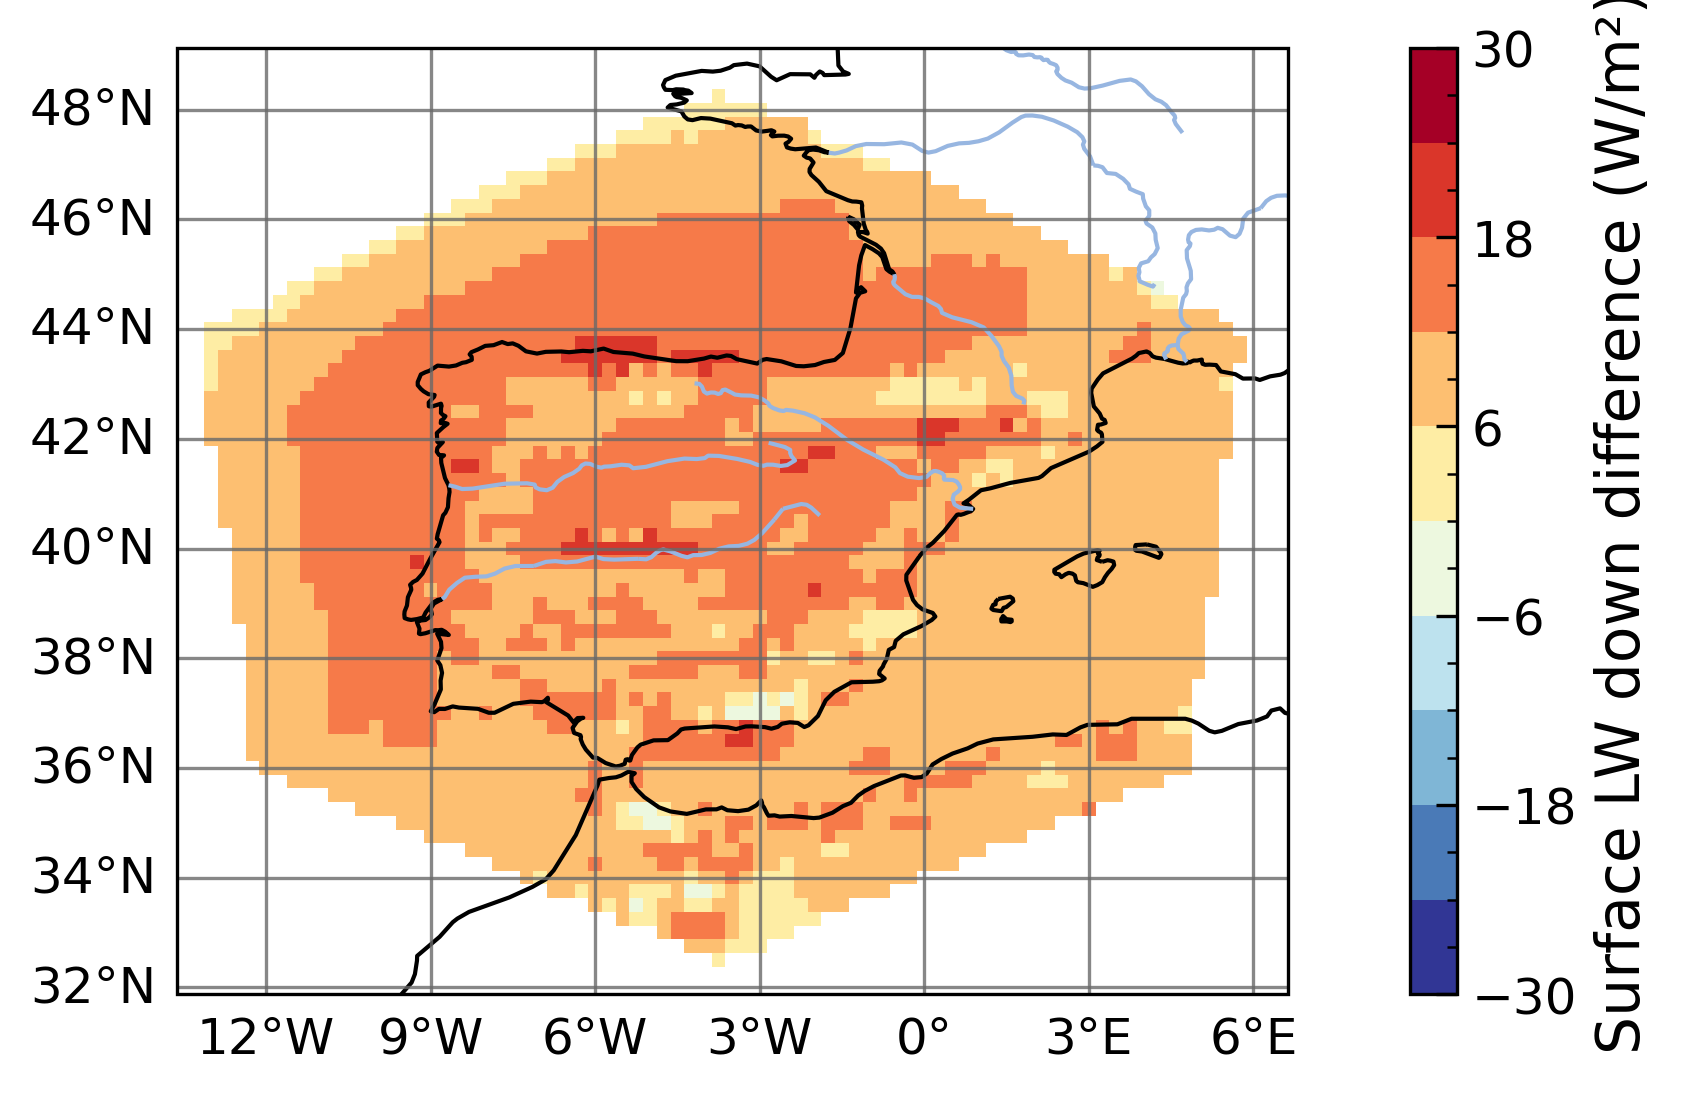
\includegraphics[width=\textwidth]{images/chap4/forcing_source/diff_map_LWdnSFC_ico_era.png}
        \end{subfigure}
    \end{tabular}
    \caption{Biases of precipitation, evapotranspiration, and downwelling radiative fluxes for the simulations \forcingERA and \forcingICO, compared to ERA5, (2010-2022).}
    \label{fig:forcing_source_ERA_diff_maps_endvars}
\end{figure}

Two simulations using the small simulation domain over the period 2010-2022 were compared to assess the influence of the source used for the lateral forcing: one with forcing data from the ERA5 reanalysis (\forcingERA) and one using outputs of a global ICOLMDZOR simulation as forcing data (\forcingICO). 
Simulation \forcingICO were run by Frédérique Cheruy, and Mariame Maiga contributed to the preliminary analysis during her internship.

\hfill

In the transition zone, the biases in precipitation and downwelling shortwave flux compared to ERA5 are much smaller in \forcingICO (Fig. \ref{fig:forcing_source_ERA_diff_maps_endvars}a, b, e, f) and much more clearly limited to the edges of the domain. For these variables, as well as for the downwelling longwave flux (Fig. \ref{fig:forcing_source_ERA_diff_maps_endvars}g, h), the spatial pattern of the bias to ERA5 is similar to the patterns seen in simulations with the intermediate or large domain (Fig. \ref{fig:domain_size_P_ET_ERA_diff_maps} \ref{fig:domain_size_clouds_ERA_diff_maps}) confirming the idea that the model is much more consistent than when it is forced by ERA. 
For ET over the Atlantic ocean, there is no clear improvement, but over the Mediterranean, the underestimation is reversed to a small overestimation, as also seen in simulations with larger domains (Fig. \ref{fig:domain_size_P_ET_ERA_diff_maps}e, f).
All these findings confirm that the LAM can be influenced by the source used for the lateral forcing, and that forcing it with data from a global ICOLMDZOR simulation rather than ERA5 allows a more consistent behaviour of the condensation scheme in the transition zone, and avoids the spread of the biases from the edges of the domain to the central free zone.

\hfill

However, it remains important to note that in general, the global ICOLMDZOR simulation is not as realistic as ERA5 and may induce new biases in the simulation, especially when studying short periods of time where interannual variability can lead to large differences between reality and the simulation. 
In \forcingICO, over the Iberian Peninsula, precipitation is clearly overestimated in northern mountainous areas (Fig. \ref{fig:forcing_source_ERA_diff_maps_endvars}b), while the larger low cloud cover affects downwelling radiative fluxes along the Atlantic coast, leading to an underestimation of the shortwave flux and an overestimation of the longwave flux (Fig. \ref{fig:forcing_source_ERA_diff_maps_endvars}f, h).

To assess the consequences of these new biases over the study area, precipitation and ET in the two simulation were respectively compared to the GPCC and GLEAM products over the Iberian Peninsula, from 2010 to 2019.
When forced with ICOLMDZ rather than ERA5, the LAM keeps the same level of performance in spring and largely improves from July to October (Fig. \ref{fig:forcing_source_SC}a). This improvement is possible because the precipitation underestimation in the transition zone is largely reduce and does not affect the central part of the domain. However, in winter, the LAM now strongly overestimates precipitation, mainly due to excessive snow and rainfall in the mountainous areas as visible in Fig. \ref{fig:forcing_source_ERA_diff_maps_endvars}b. This is a known bias of climate models and was already described for the LMDZ physics in particular \citep{arjdal_modeling_2024, adhikari_evaluation_2024}. Over this season, model performance may not be improved by changing the forcing source, but it has the advantage of being self-consistent over the domain, and of producing biases that have already been studied and analysed in the IPSL modelling community.

The increases in summer precipitation in \forcingICO translate into increases in ET (Fig. \ref{fig:forcing_source_SC}b), although a gap remains between the GLEAM product and the model, which might derive from various causes: an underestimation of the downwelling shortwave radiation in some regions, the parameterization of evapotranspiration components in the land surface model, the absence of irrigation in the simulations. In other seasons, the difference between the two simulation remains limited. In particular, the increases in precipitation in winter do not lead to significant changes in ET since in the moutainous areas where they occur, precipitation is already large and ET is not limited by the available soil moisture.

\hfill

To summarise, the comparison of the two LAM simulations, \forcingERA and \forcingICO, corroborated the hypothesis that the inconsistent behaviour of the LAM in the transition zone was due to discrepancies between the physics used to produce the ERA5 reanalysis and the LMDZ physics of the LAM. Indeed, biases on the edges of the domain are largely reduced when the model used ICOLMDZ outputs as forcing data, and their influence on the Iberian Peninsula almost disappears. However, although the LAM gains consistency, its performance compared to observation-based reference products may not be systematically improved, because the ICOLMDZ model has its own biases, that can be present in the forcing and amplified by the LAM, as seen with the overestimation of precipitation over mountainous areas in winter.

%figure : SC of precip and evap with GLEAM and GPCC
\begin{figure}[htbp]
    \centering
    %precip
    \begin{subfigure}[b]{0.49\textwidth}
        \caption{Seasonal cycle of precipitation (2010-2019)}
        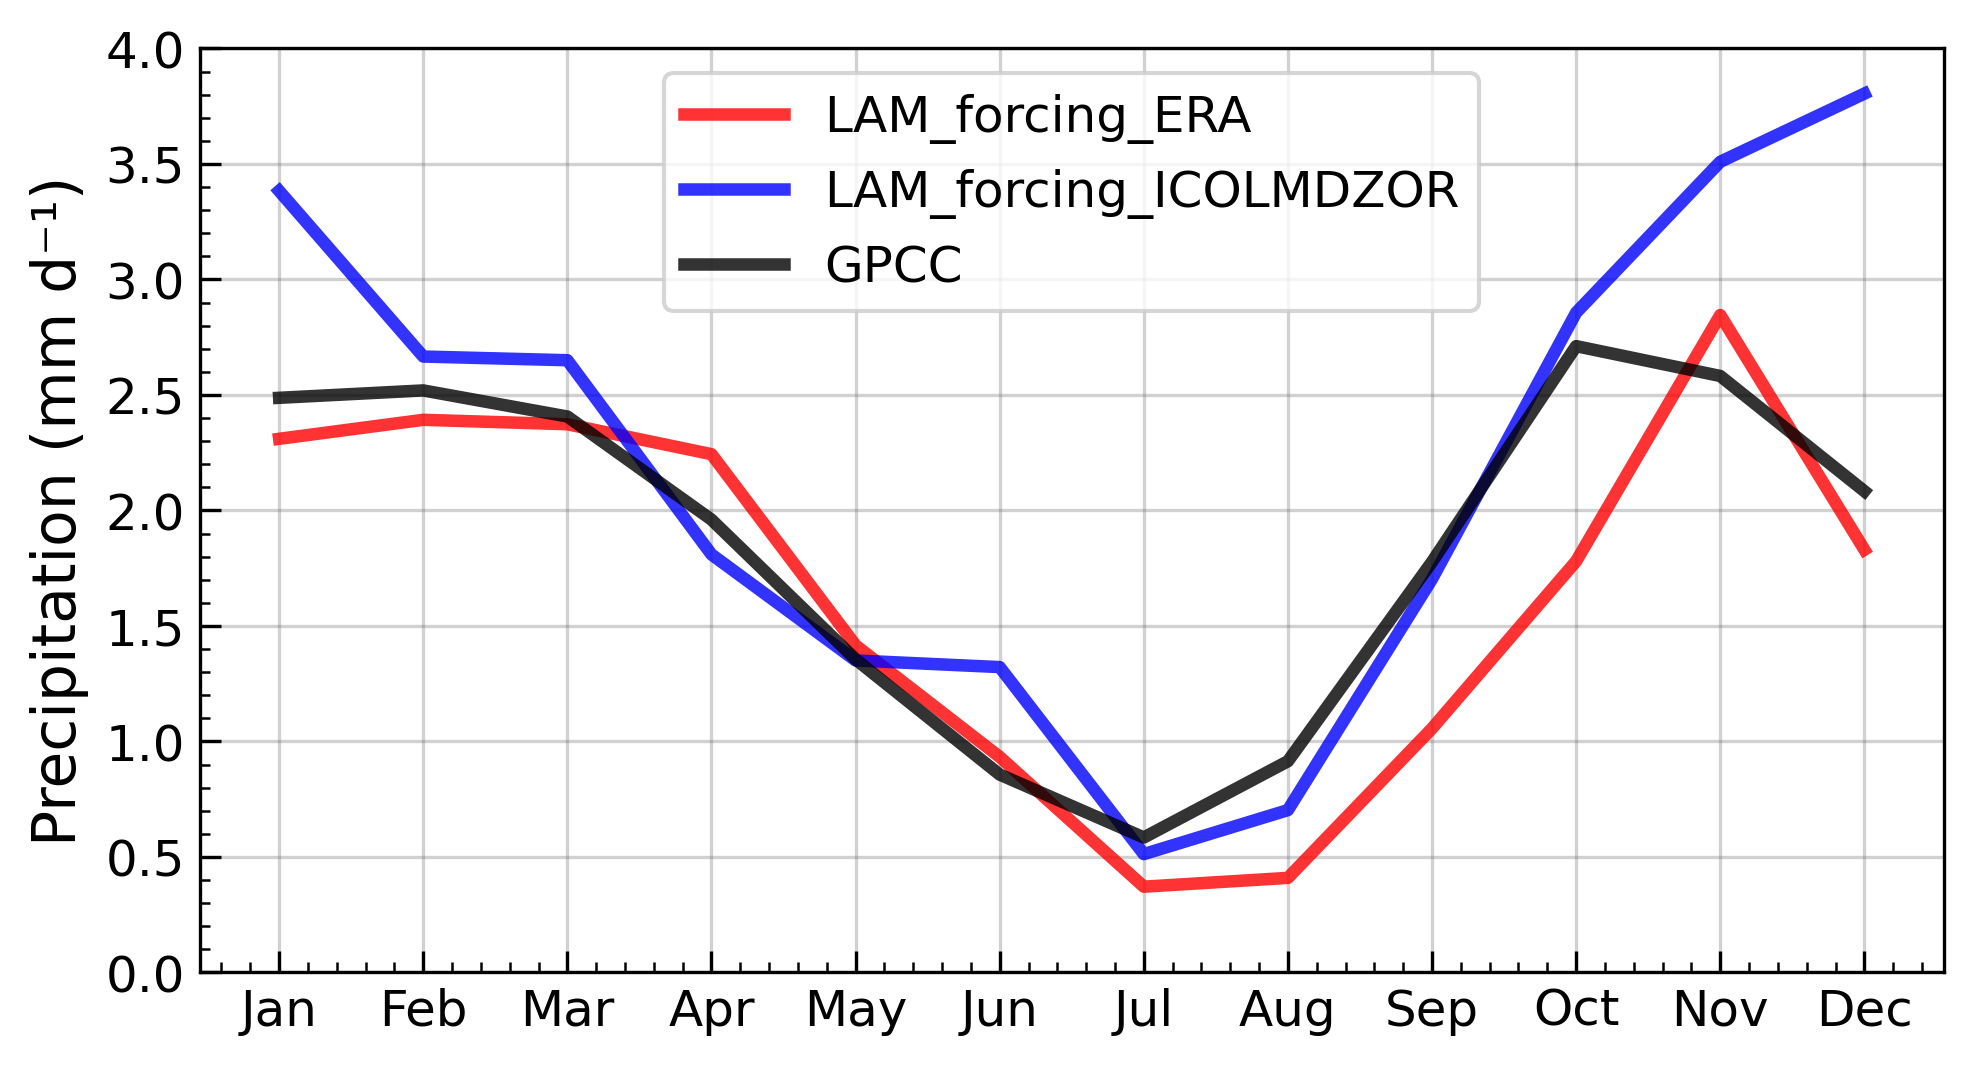
\includegraphics[width=\textwidth]{images/chap4/forcing_source/IP_seasonal_cycle_precip.png}
    \end{subfigure}
    \begin{subfigure}[b]{0.49\textwidth}
        \caption{Seasonal cycle of ET (2010-2019)}
        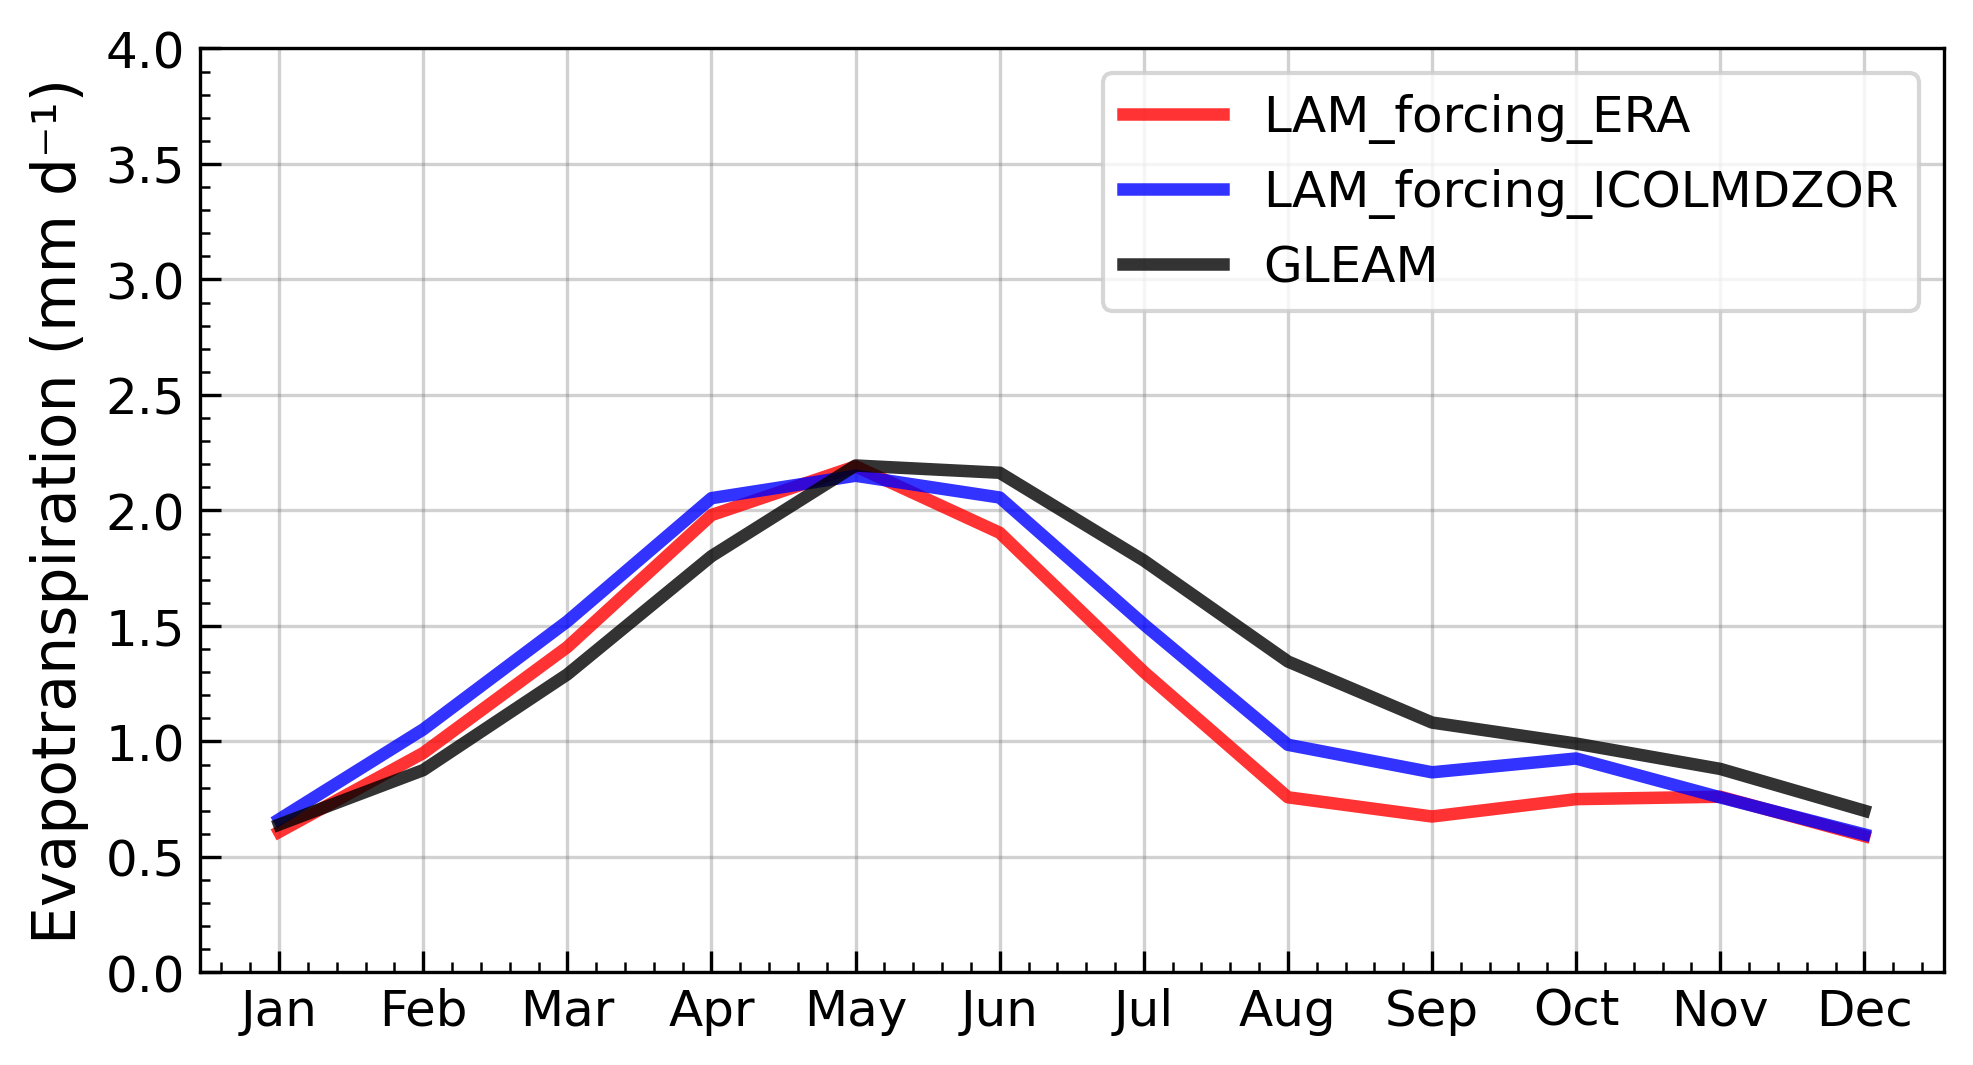
\includegraphics[width=\textwidth]{images/chap4/forcing_source/IP_seasonal_cycle_evap.png}
    \end{subfigure}
    \caption{Mean seasonal cycle of precipitation and evapotranspiration, on average over the Iberian Peninsula, for the LAM forced by ERA (red) and forced by ICOLMDZOR (blue), and the GPCC and GLEAM products (2010-2019).}
    \label{fig:forcing_source_SC}
\end{figure}

\clearpage

\section{Impact of the forcing file sampling frequency}
\label{sec:forcing_frequency}
%figure : maps of diff vs ERA for 2 forcing sampling freqs
\begin{figure}[!h]
    \centering
    \begin{tabular}{cc}
        %precip
        \begin{subfigure}[b]{0.33\textwidth}
            \caption{Precipitation bias\\(mm \perday, \forcingoneh)}
            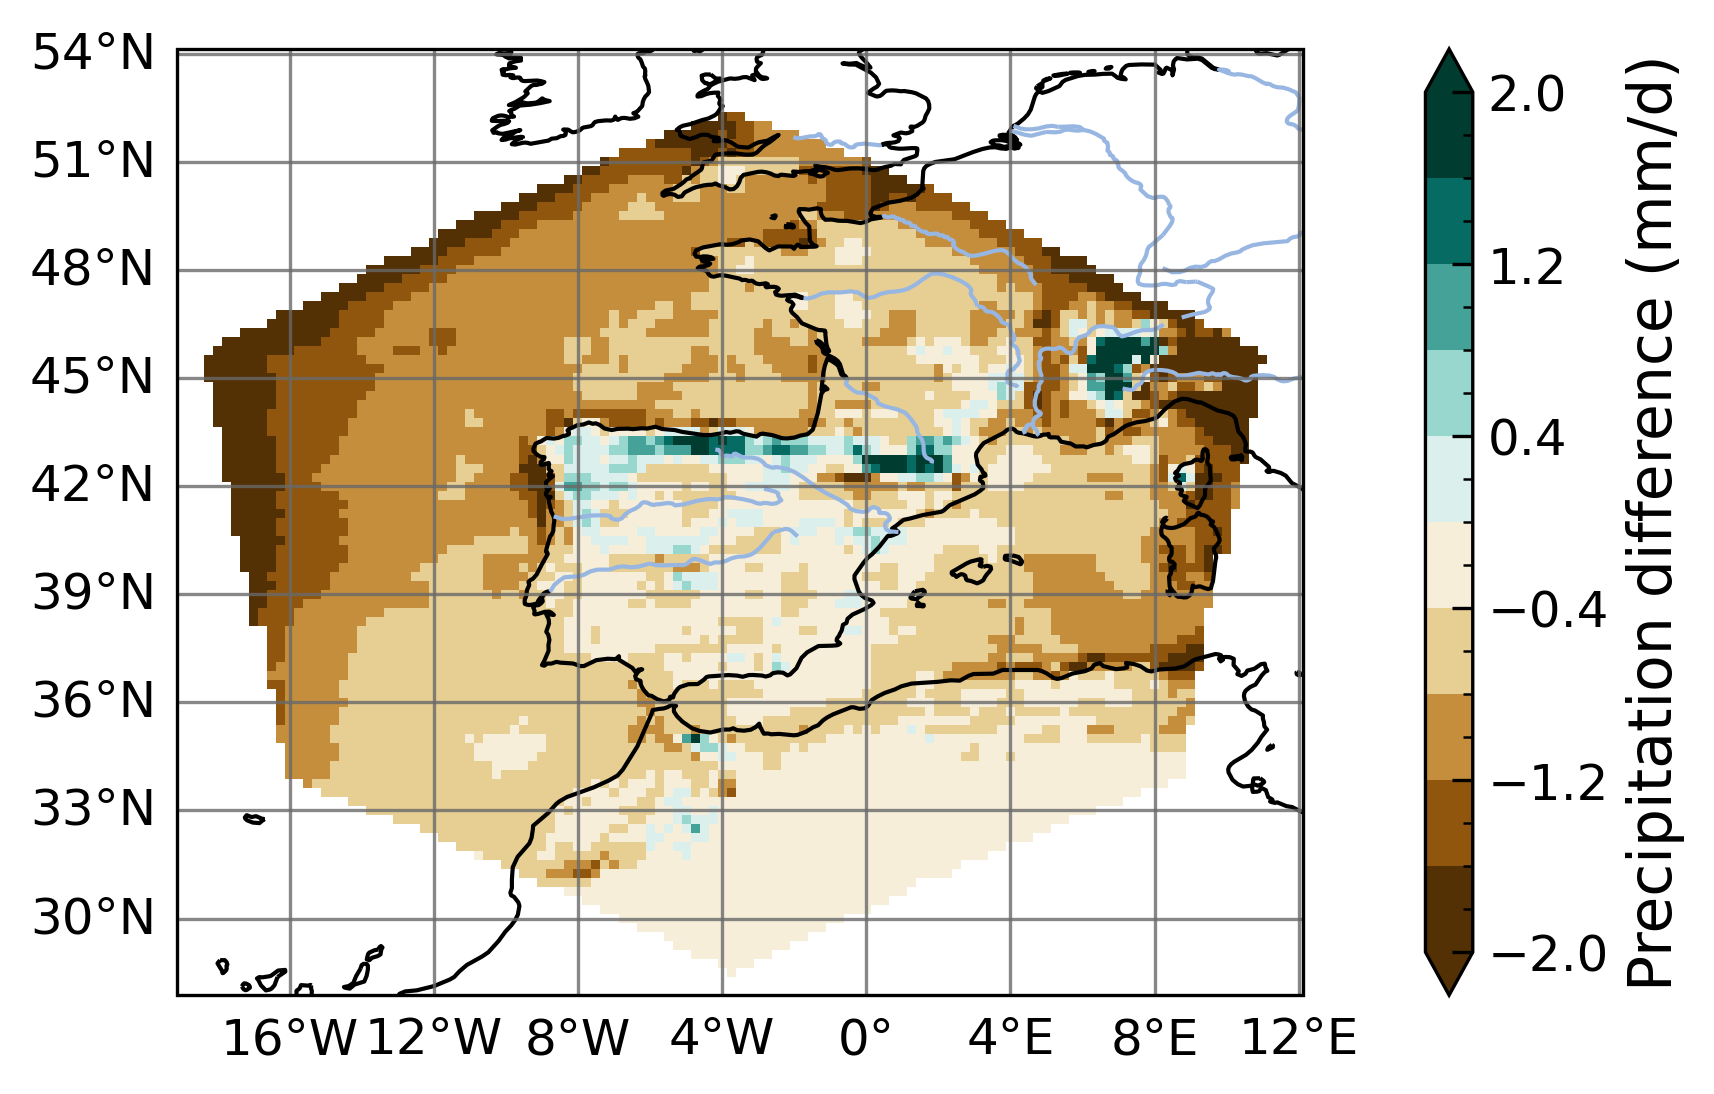
\includegraphics[width=\textwidth]{images/chap4/forcing_sampling_freq/diff_map_precip_lmdz1h_era.png}
        \end{subfigure} &
        \begin{subfigure}[b]{0.33\textwidth}
            \caption{Precipitation bias\\(mm \perday, \forcingsixh)}
            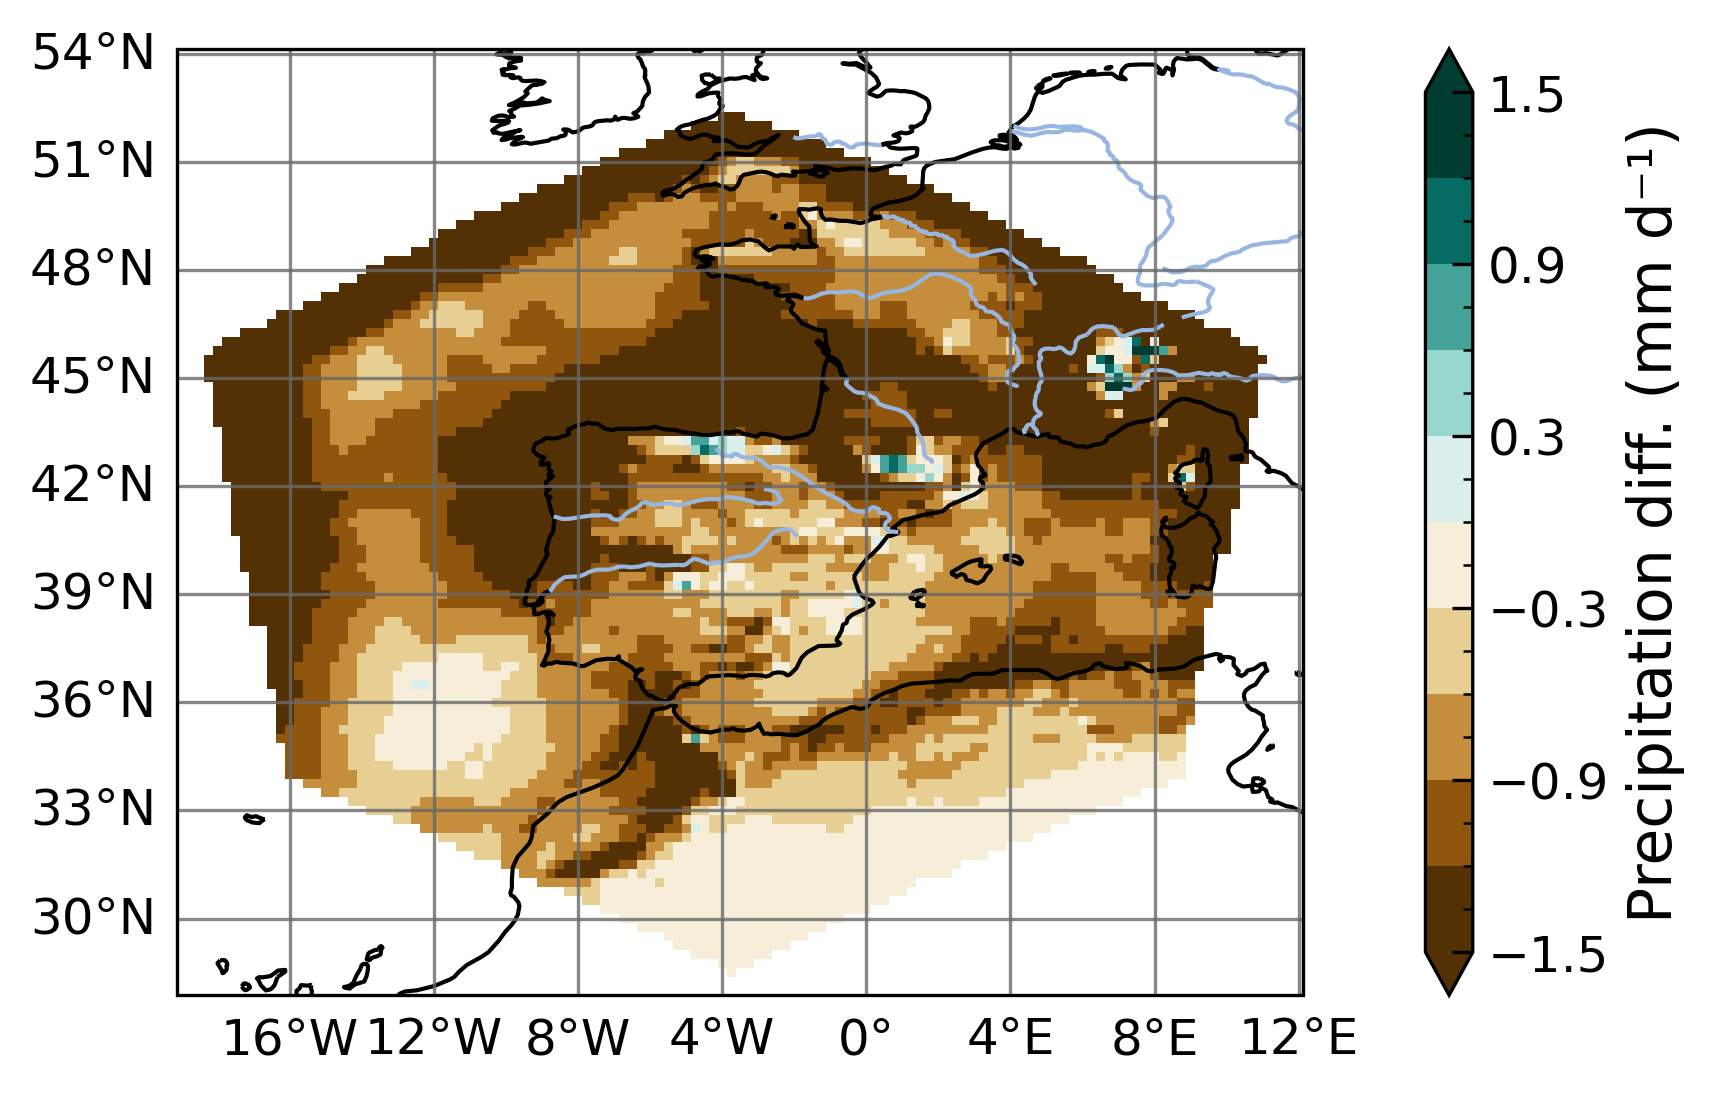
\includegraphics[width=\textwidth]{images/chap4/forcing_sampling_freq/diff_map_precip_lmdz6h_era.png}
        \end{subfigure} \\
        
        %evap
        \begin{subfigure}[b]{0.33\textwidth}
            \caption{ET bias\\(mm \perday, \forcingoneh)}
            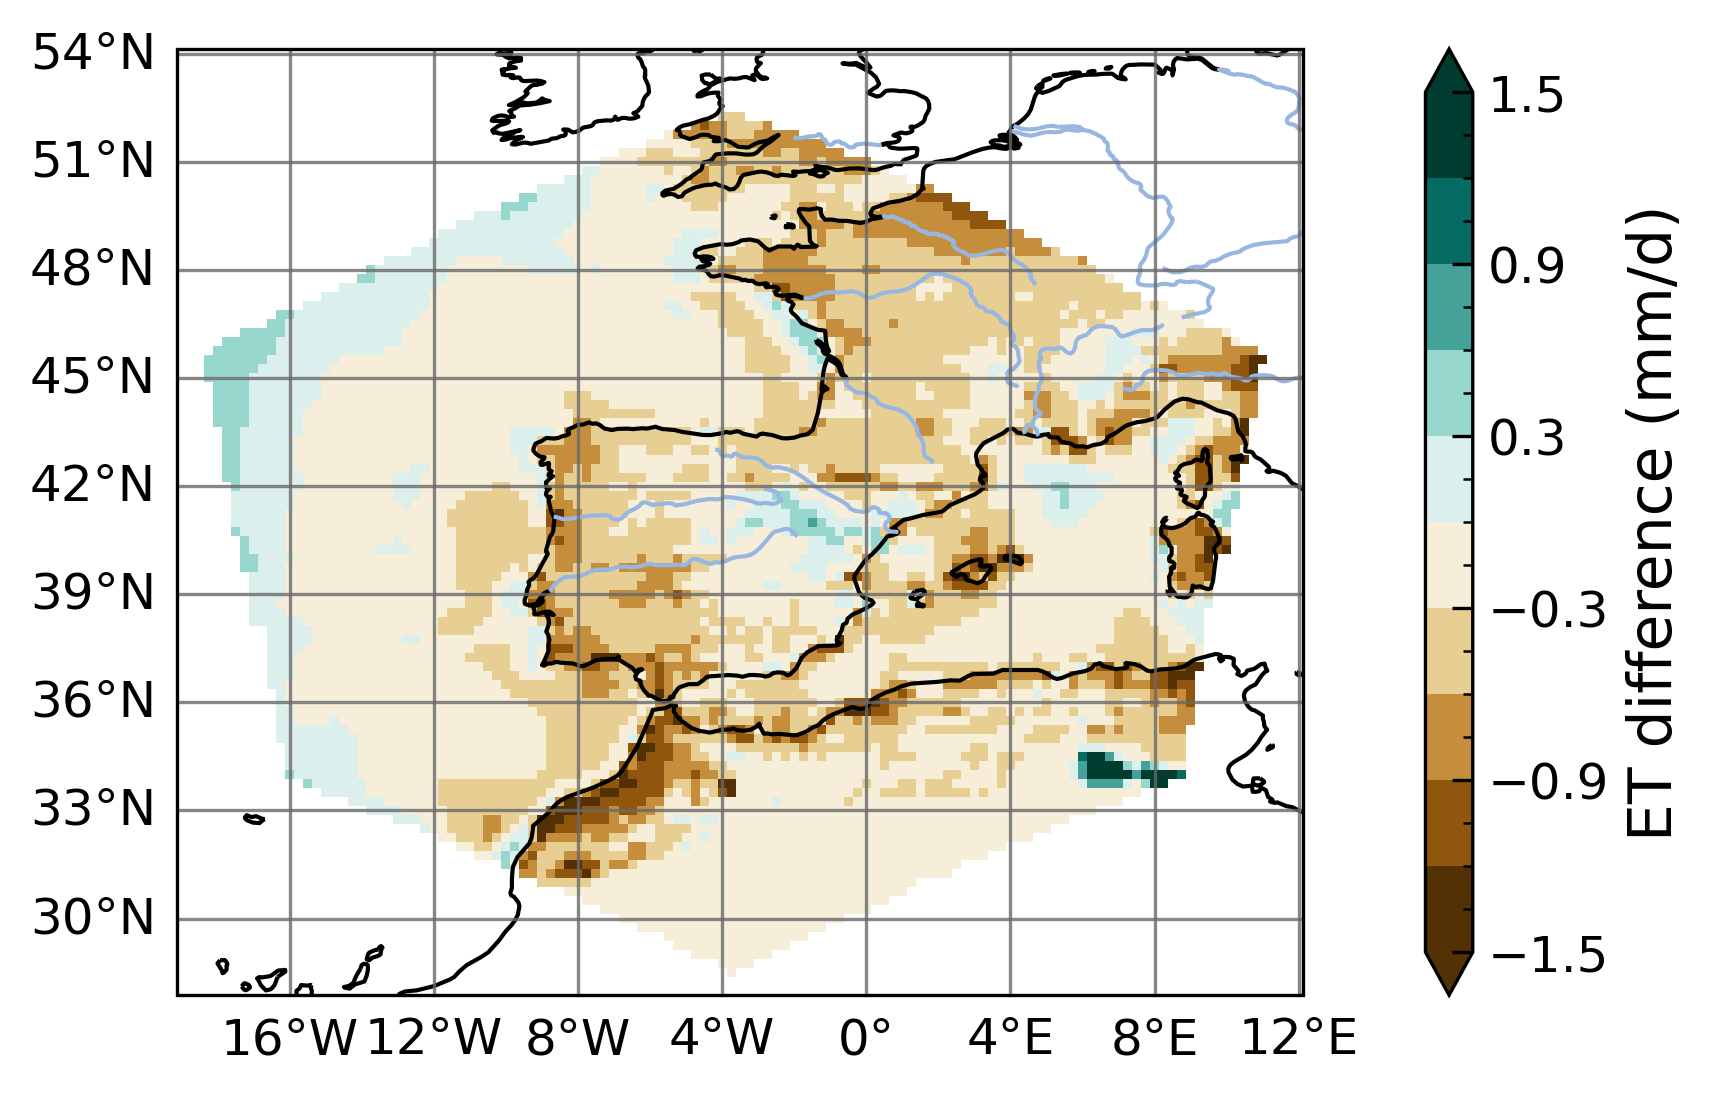
\includegraphics[width=\textwidth]{images/chap4/forcing_sampling_freq/diff_map_evap_lmdz1h_era.png}
        \end{subfigure} &
        \begin{subfigure}[b]{0.33\textwidth}
            \caption{ET bias\\(mm \perday, \forcingsixh)}
            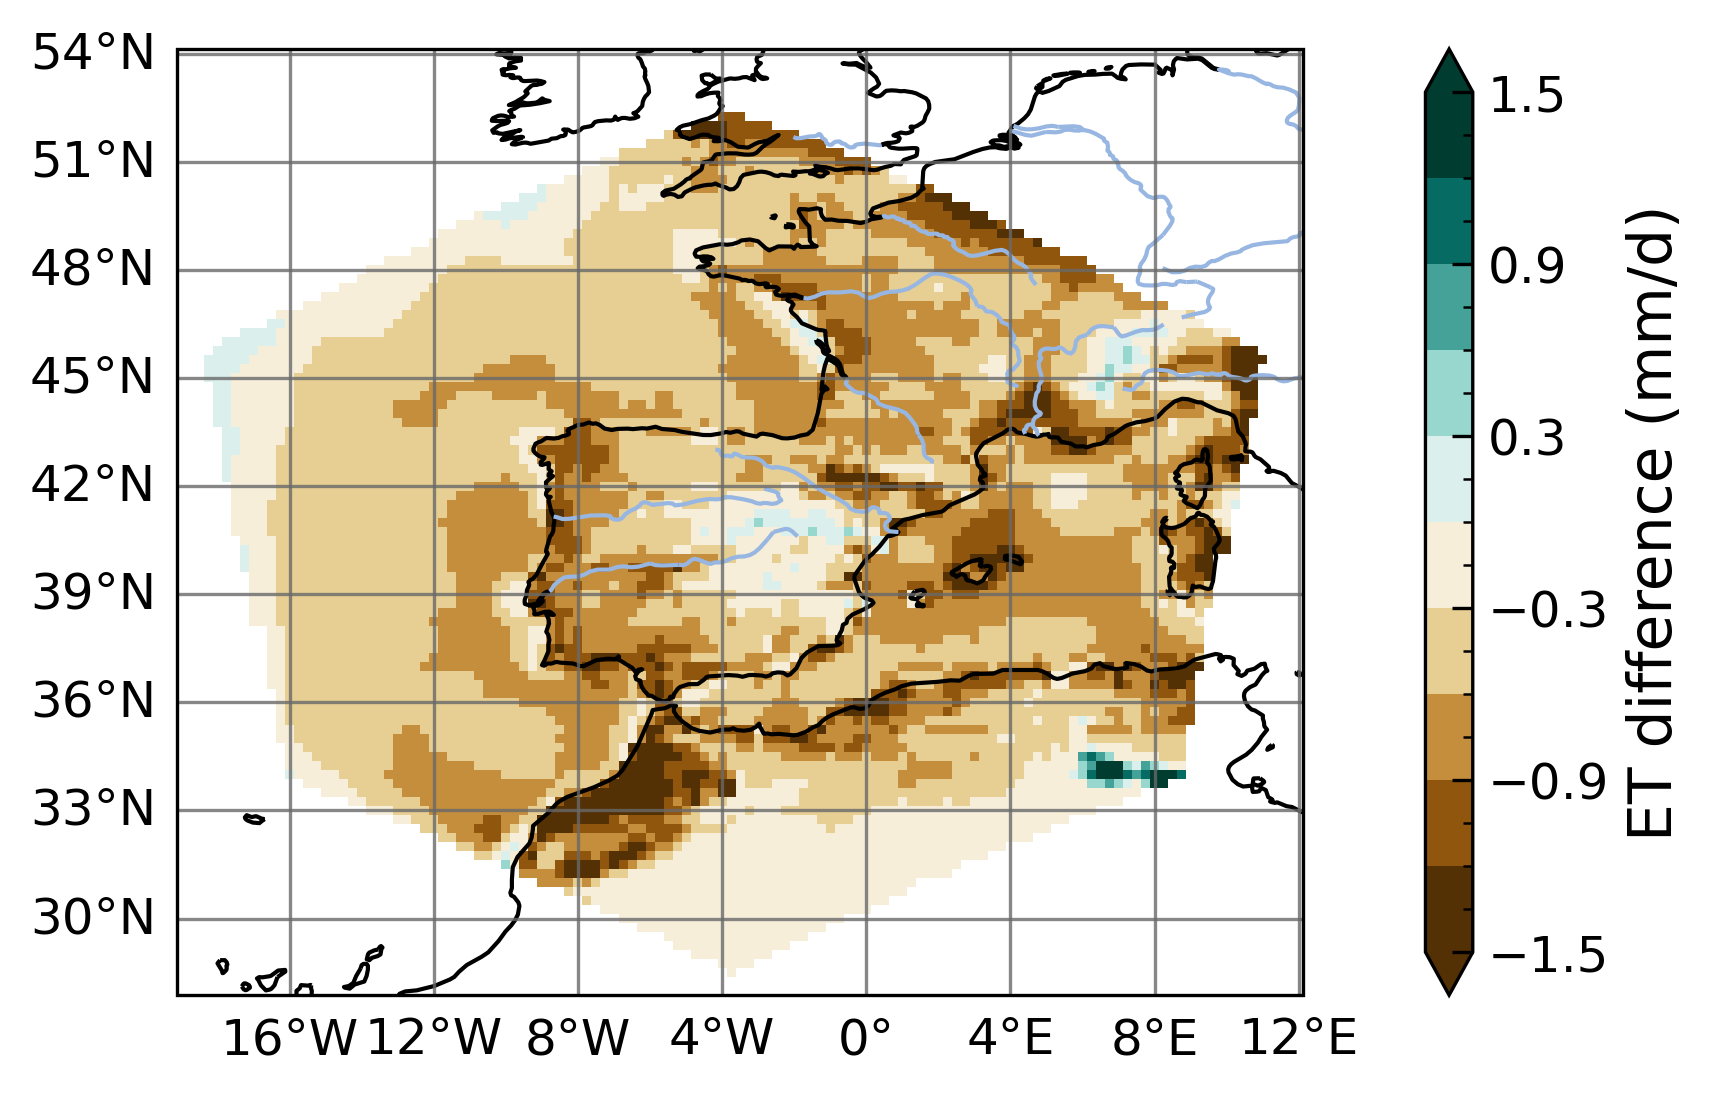
\includegraphics[width=\textwidth]{images/chap4/forcing_sampling_freq/diff_map_evap_lmdz6h_era.png}
        \end{subfigure} \\
        
        %SWdn
        \begin{subfigure}[b]{0.33\textwidth}
            \caption{Downwelling SW flux bias\\(W \persqm, \forcingoneh)}
            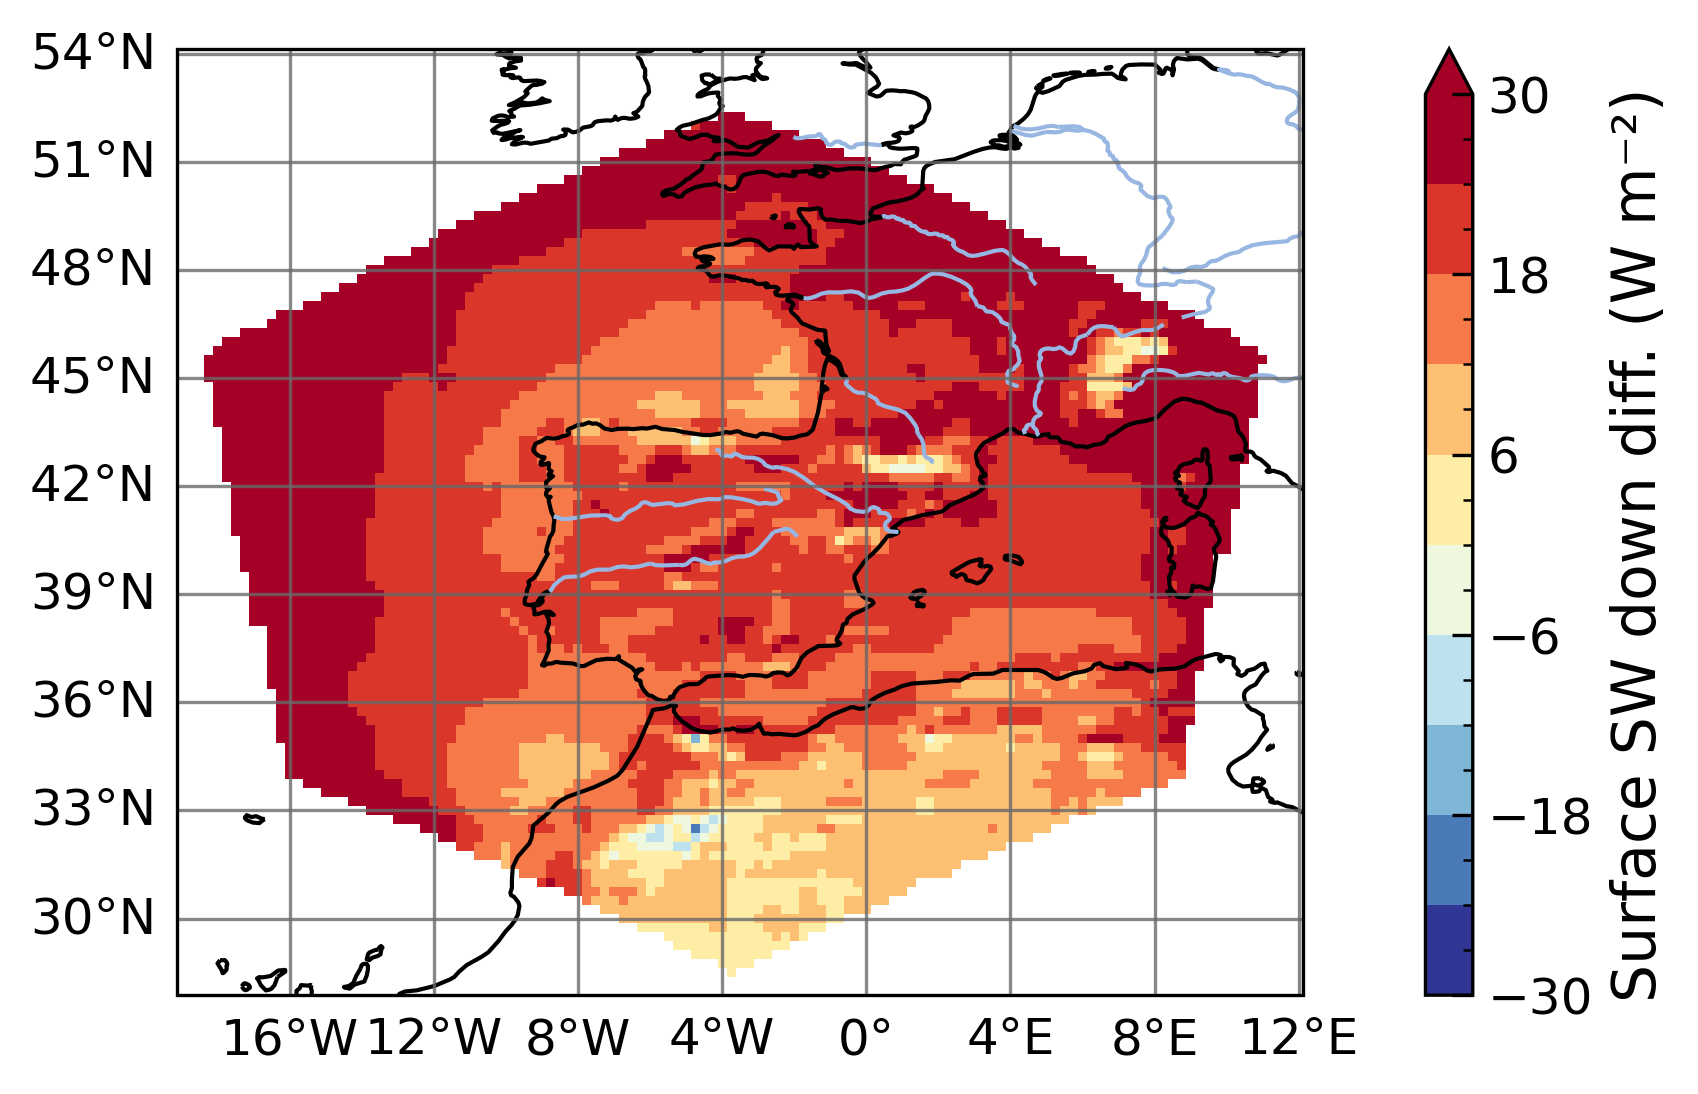
\includegraphics[width=\textwidth]{images/chap4/forcing_sampling_freq/diff_map_SWdnSFC_lmdz1h_era.png}
        \end{subfigure} &
        \begin{subfigure}[b]{0.33\textwidth}
            \caption{Downwelling SW flux bias\\(W \persqm, \forcingsixh)}
            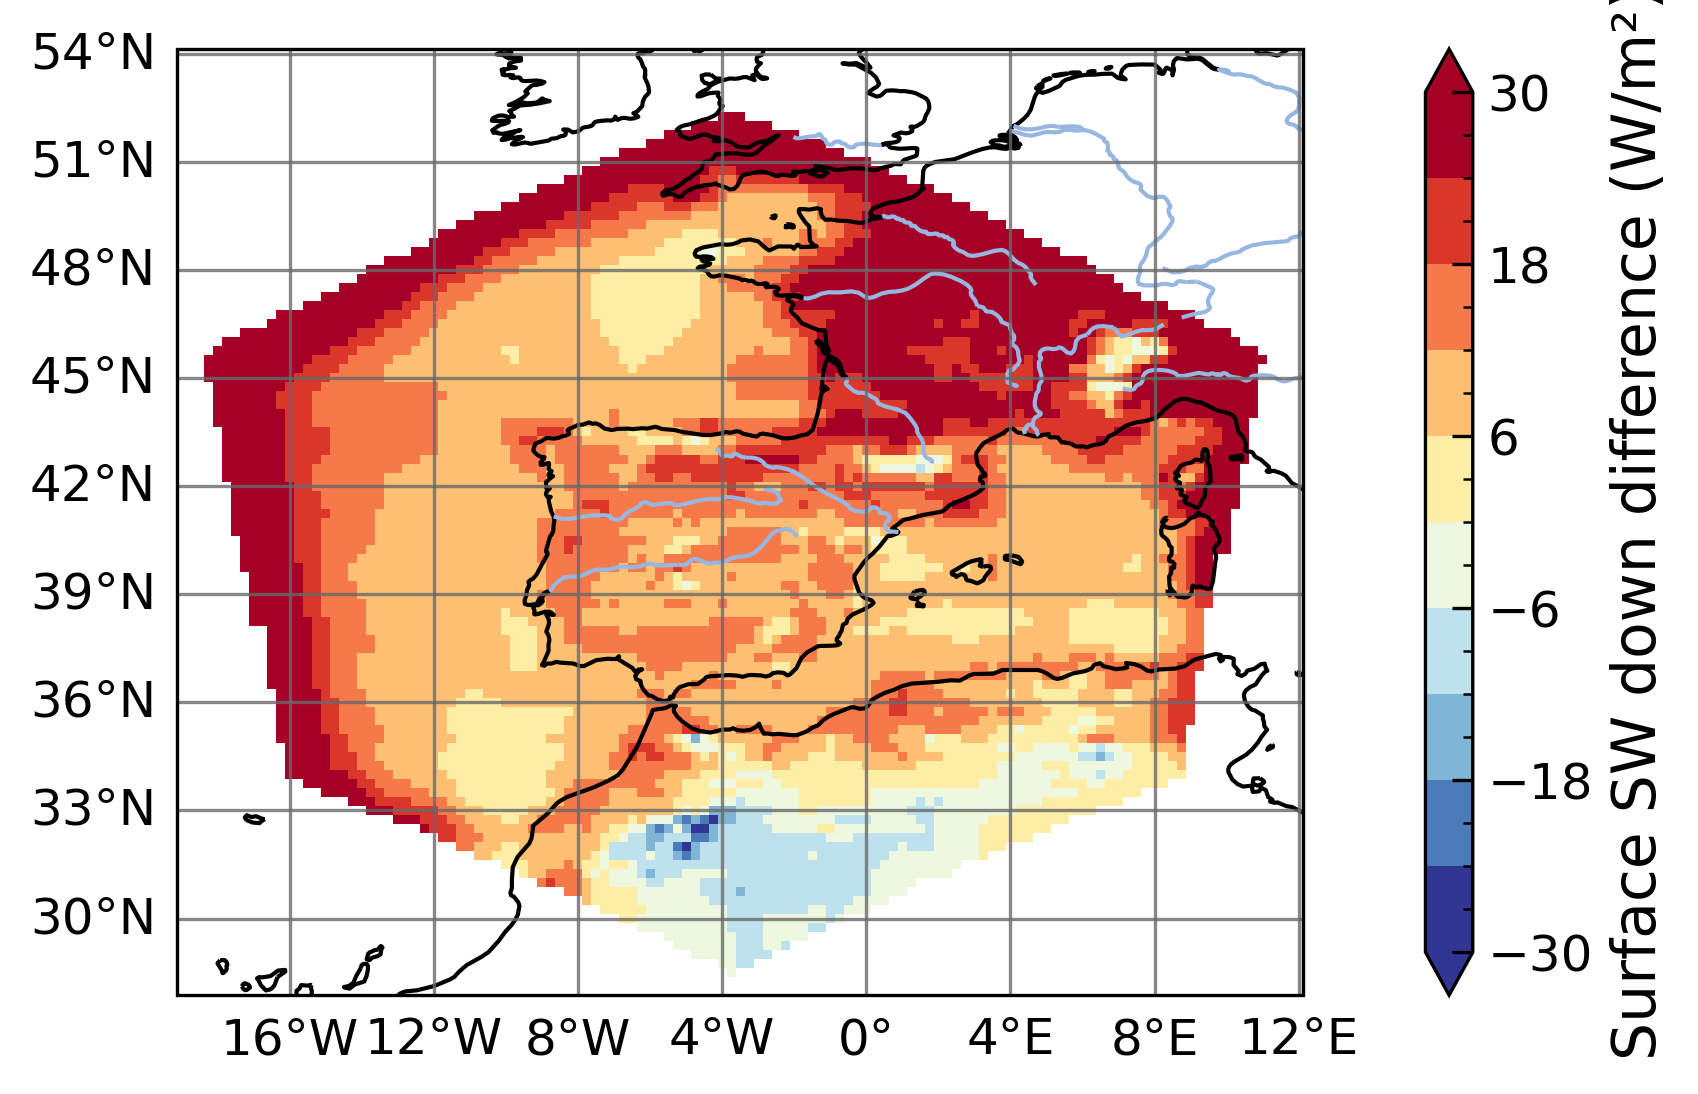
\includegraphics[width=\textwidth]{images/chap4/forcing_sampling_freq/diff_map_SWdnSFC_lmdz6h_era.png}
        \end{subfigure}\\
        
        %LWdn
        \begin{subfigure}[b]{0.33\textwidth}
            \caption{Downwelling LW flux bias\\(W \persqm, \forcingoneh)}
            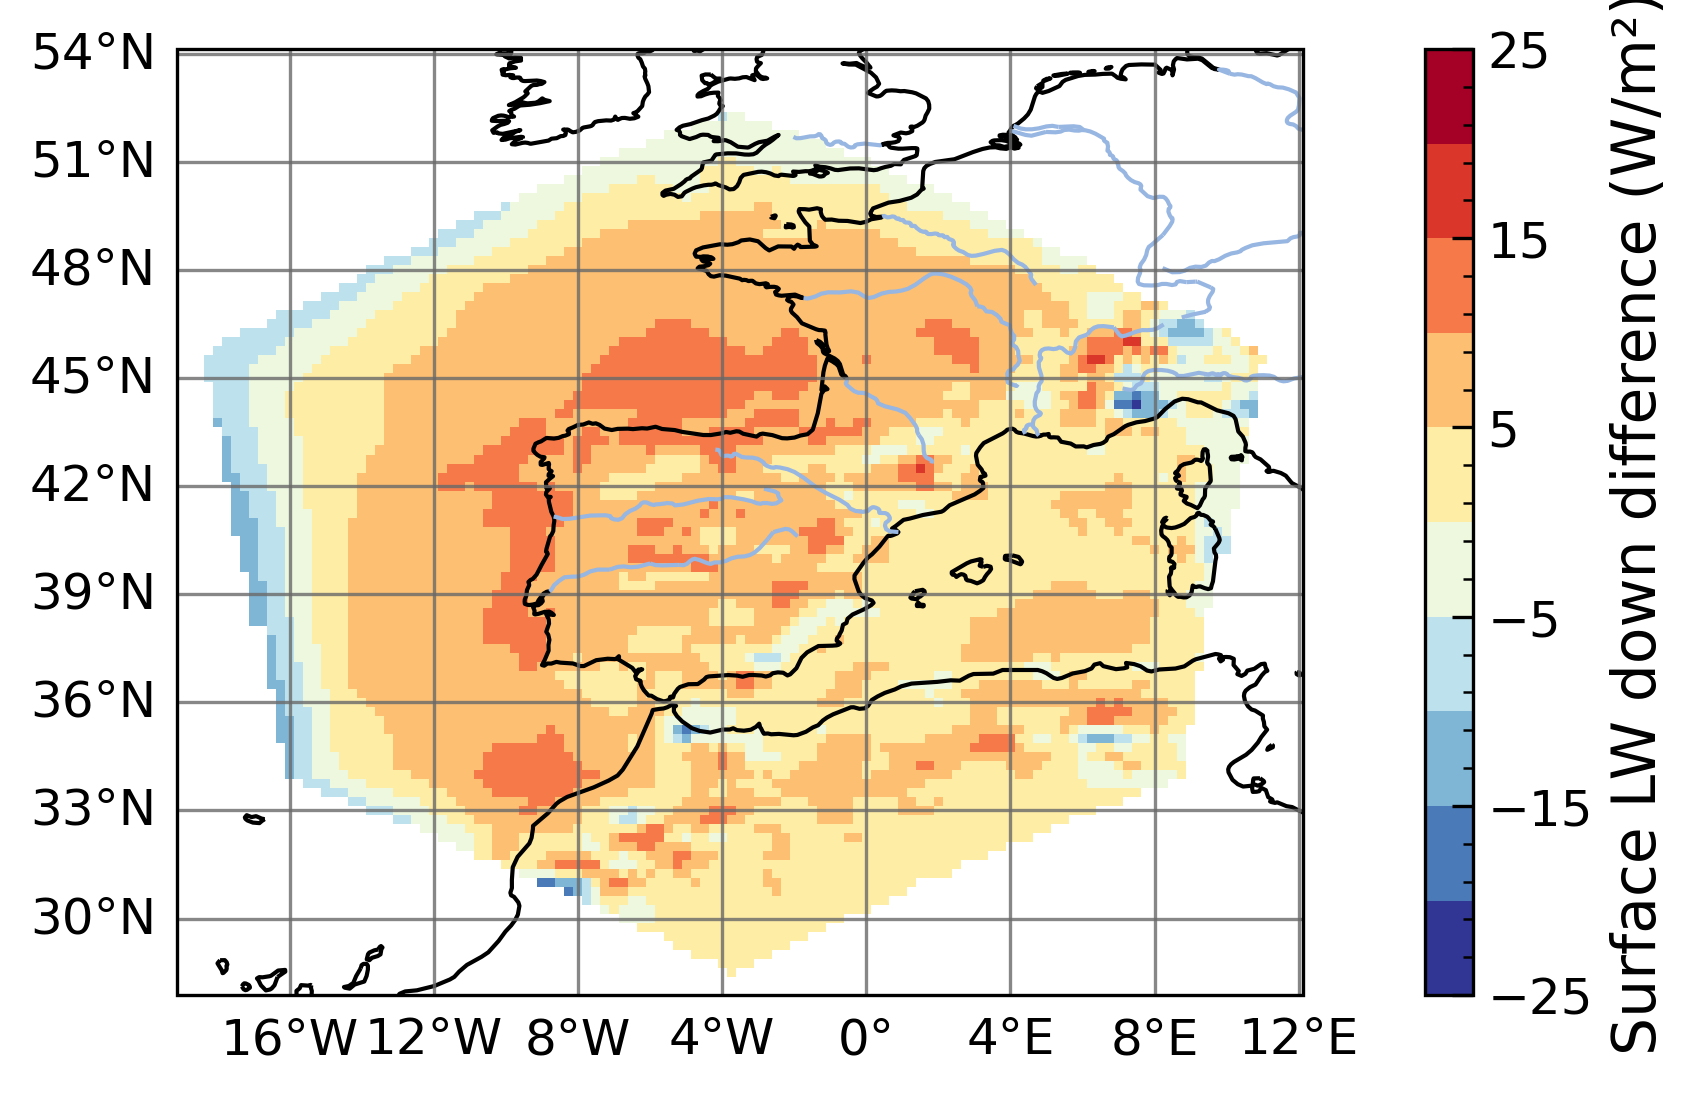
\includegraphics[width=\textwidth]{images/chap4/forcing_sampling_freq/diff_map_LWdnSFC_lmdz1h_era.png}
        \end{subfigure} &
        \begin{subfigure}[b]{0.33\textwidth}
            \caption{Downwelling LW flux bias\\(W \persqm, \forcingsixh)}
            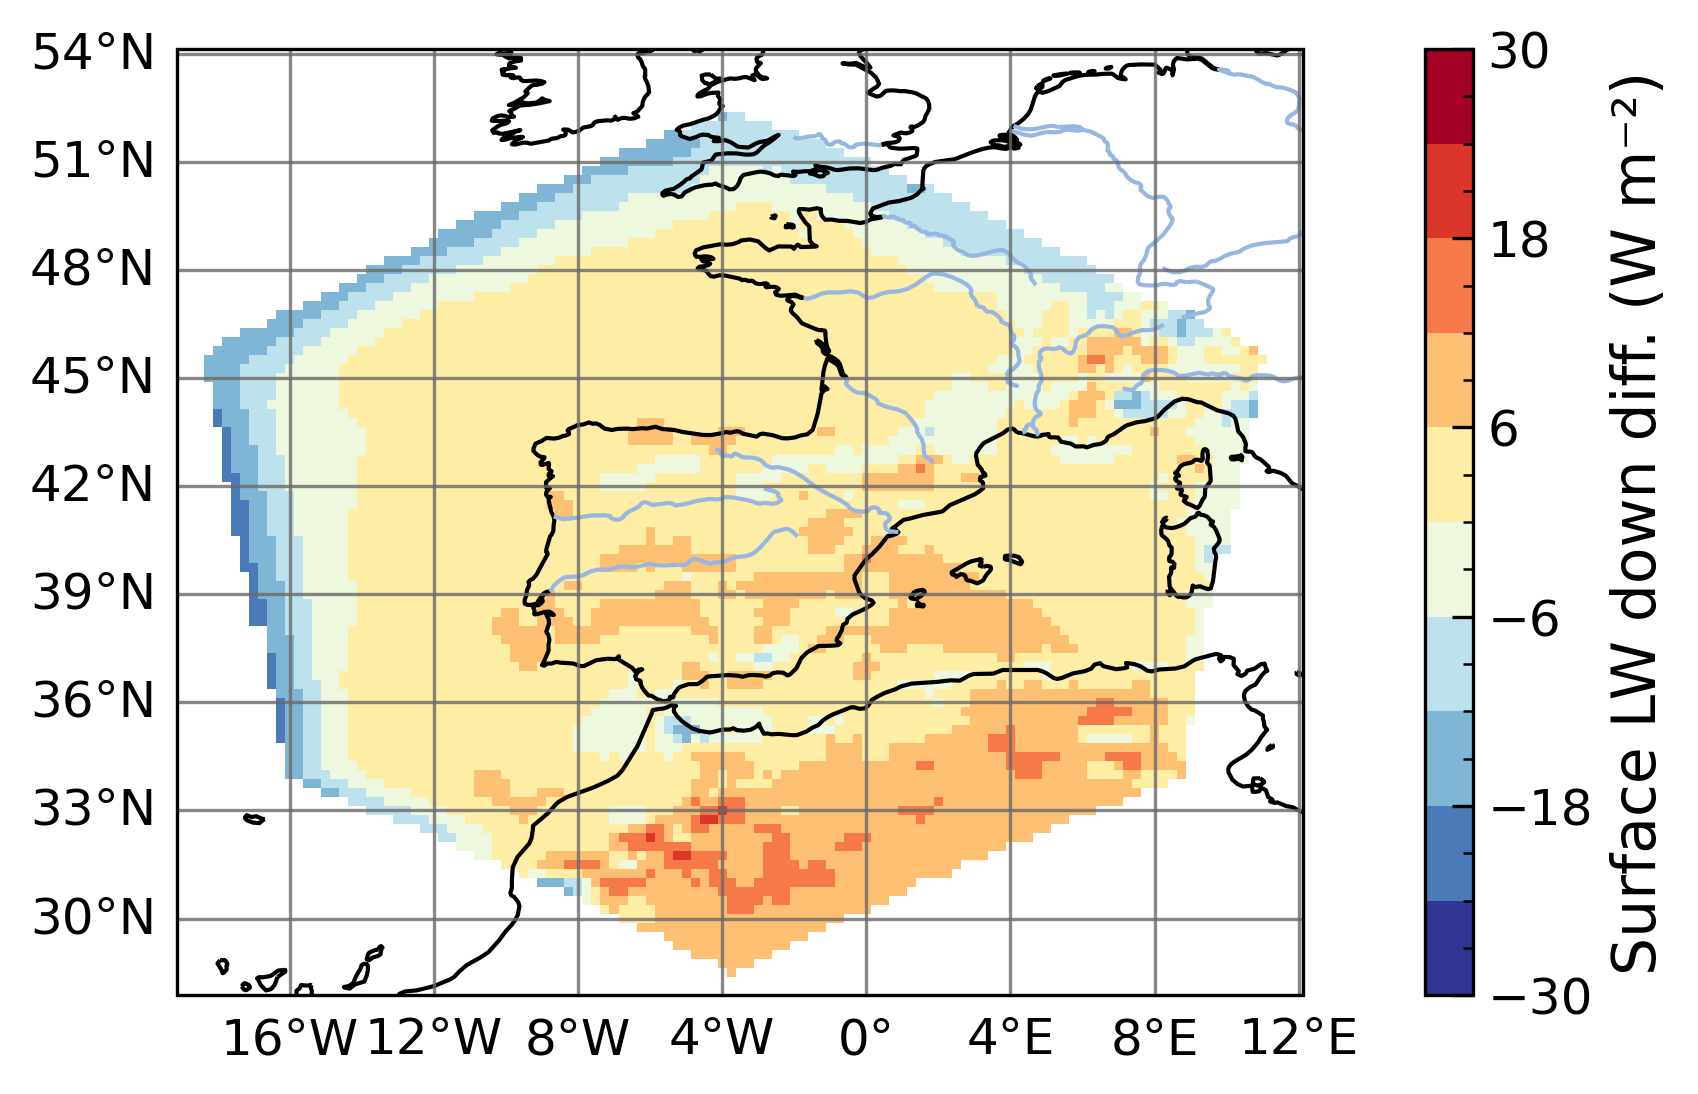
\includegraphics[width=\textwidth]{images/chap4/forcing_sampling_freq/diff_map_LWdnSFC_lmdz6h_era.png}
        \end{subfigure} \\
    \end{tabular}
    \caption{Biases of precipitation, evapotranspiration, and downwelling radiative fluxes for the two simulations, with hourly and 6-hourly forcing data, compared to ERA (2013).}
    \label{fig:forcing_sampling_freq_ERA_diff_maps}
\end{figure}

For technical reasons, running long LAM simulations or simulations under future climate using CMIP outputs as a source for the forcing data would require to use a forcing file with a 6-hours sampling frequency rather than one hour. 
Although the simulations used in this manuscript were eventually all run with hourly forcing data, an experiment was conducted to assess the effects of the forcing file sampling frequency on the LAM. 
The results presented here compare two simulations with the intermediate domain size and lateral forcing data from ERA5, one with hourly data (\forcingoneh), one with 6-hourly data (\forcingsixh). Technical issues were encountered when trying to run with 6-hourly forcing data and only the year 2013 could be run without problems. Therefore, this single year was simulated ten times in a row in each simulation setup, constituting two small simulation ensembles.

\hfill

First, it is clear that the biases in the transition zone studied in Section \ref{sec:domain_size}, are strengthened for precipitation and downwelling radiative fluxes in \forcingsixh (Fig. \ref{fig:forcing_sampling_freq_ERA_diff_maps}b, f, h). To understand it, one must remember that a lower forcing file sampling frequency does not mean the model is less constrained: variables are still nudged at every time step of the dynamics (30s), with the same intensity. However, with a lower sampling frequency, the diurnal cycle is not as well represented in the forcing data, as illustrated in Fig. \ref{fig:diurnal_cycle_sampling}. For the altitudes where variables follow a marked diurnal cycle, the inconsistencies between the LMDZ physics and the ERA5 forcing data can therefore be increased and lead to more intense biases.

\begin{figure}[htbp]
    \centering
    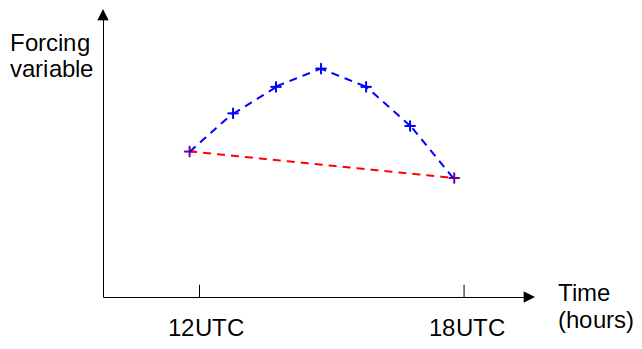
\includegraphics[width=0.5\textwidth]{images/chap4/forcing_sampling_freq/sampling_freq_diurnal_cycle.png}    
    \caption{Illustration of the differences in diurnal cycle sampling using hourly (blue) or 6-hourly (red) forcing data. Adapted from Mariame Maiga's intership defence.
    \label{fig:diurnal_cycle_sampling}}
\end{figure}

It is harder to interpret whether the biases in the transition zone have more or less impacts in the free zone with the 6-hourly forcing. For precipitation, the bias seems more confined in the transition zone over the Atlantic ocean but there is an important underestimation over France and the Iberian Peninsula (Fig. \ref{fig:forcing_sampling_freq_ERA_diff_maps}b). For downwelling radiation, it is less ambiguous as the biases are stronger in the transition zone and seem to extend over the whole domain, increasing the shortwave flux and decreasing the longwave flux (Fig. \ref{fig:forcing_sampling_freq_ERA_diff_maps}f, h)

On average over the Iberian Peninsula, the seasonal cycle of precipitation and ET have similar characteristics in both simulations but \forcingsixh presents less precipitation all year, leading to a stronger underestimation in summer, autumn and winter compared to GPCC (Fig. \ref{fig:forcing_sampling_freq_SC}a). This lower amount of precipitation induces a lower ET in the seasons where it is limited by available soil moisture, which also increases the underestimation compared to GLEAM data (Fig. \ref{fig:forcing_sampling_freq_SC}b). 

%figure : SC of precip and evap with GLEAM and GPCC
\begin{figure}[htbp]
    \centering
    %precip
    \begin{subfigure}[b]{0.49\textwidth}
        \caption{Seasonal cycle of precipitation (2013)}
        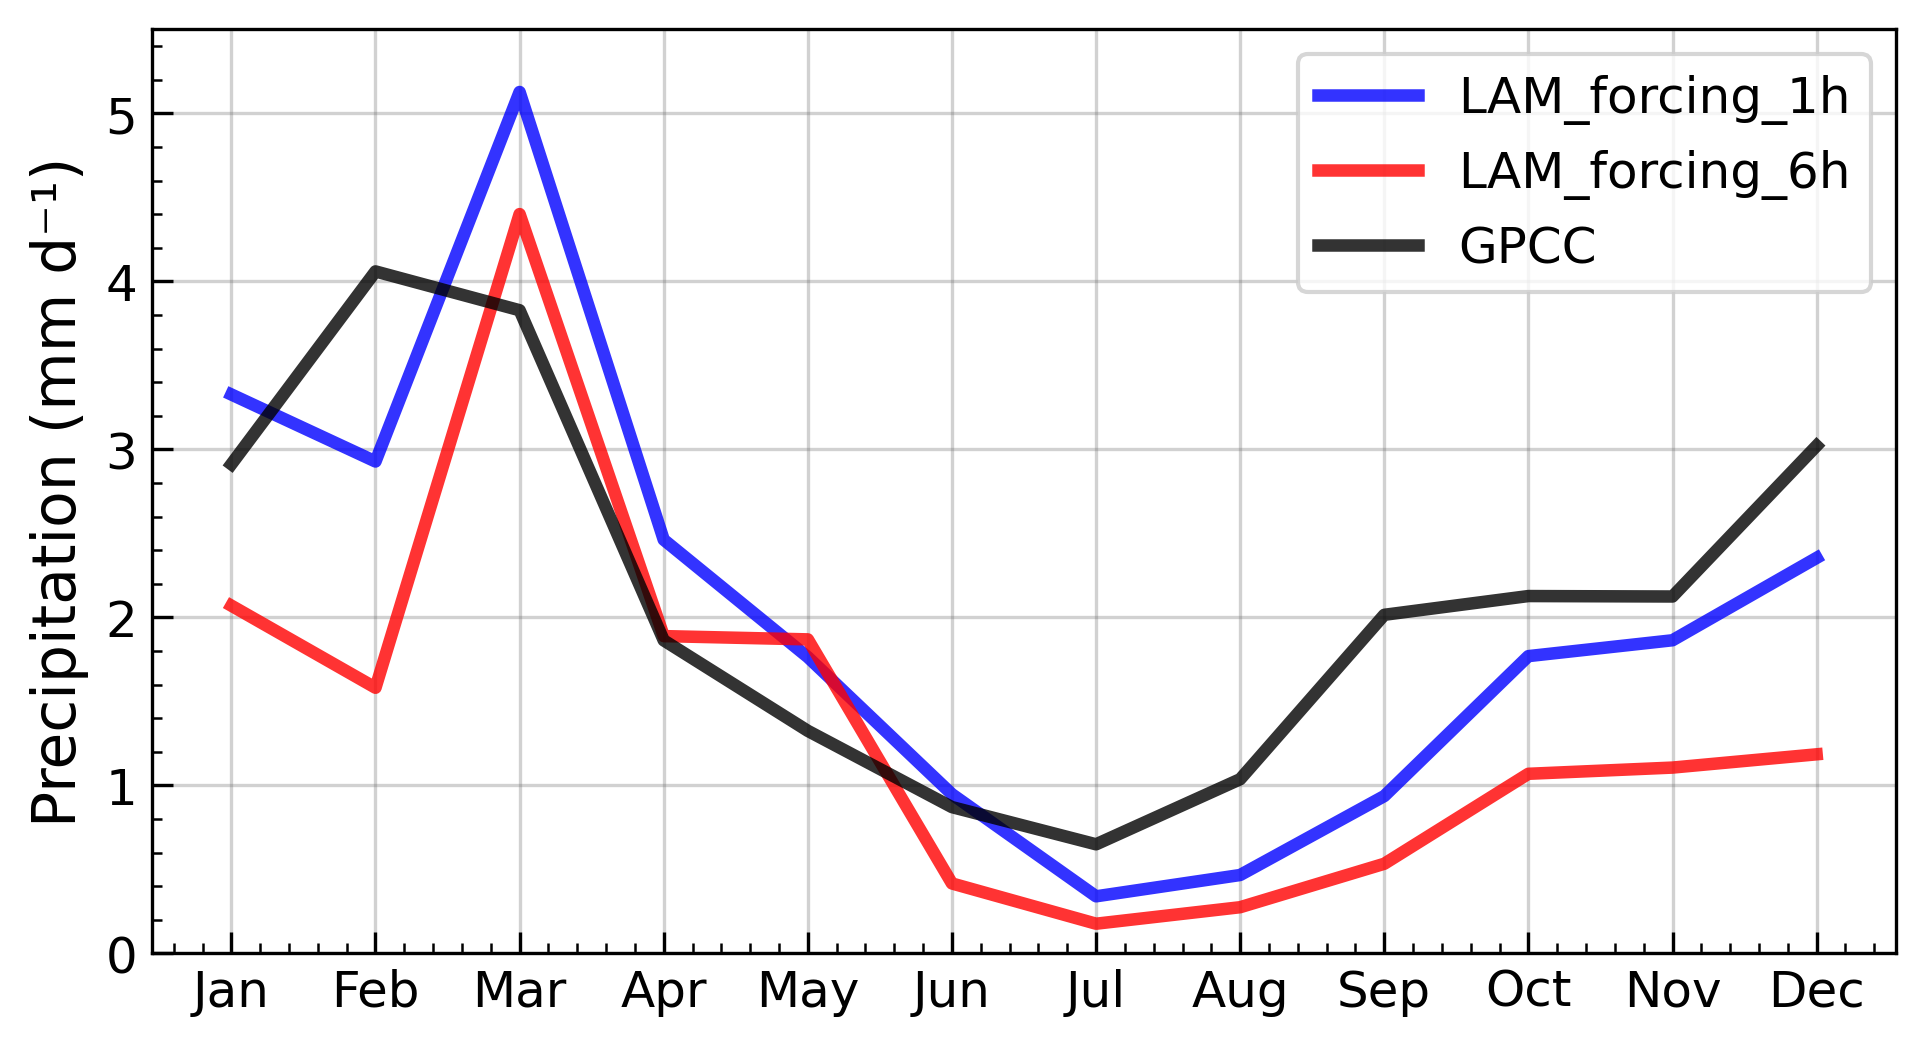
\includegraphics[width=\textwidth]{images/chap4/forcing_sampling_freq/IP_seasonal_cycle_precip.png}
    \end{subfigure}
    \begin{subfigure}[b]{0.49\textwidth}
        \caption{Seasonal cycle of ET (2013)}
        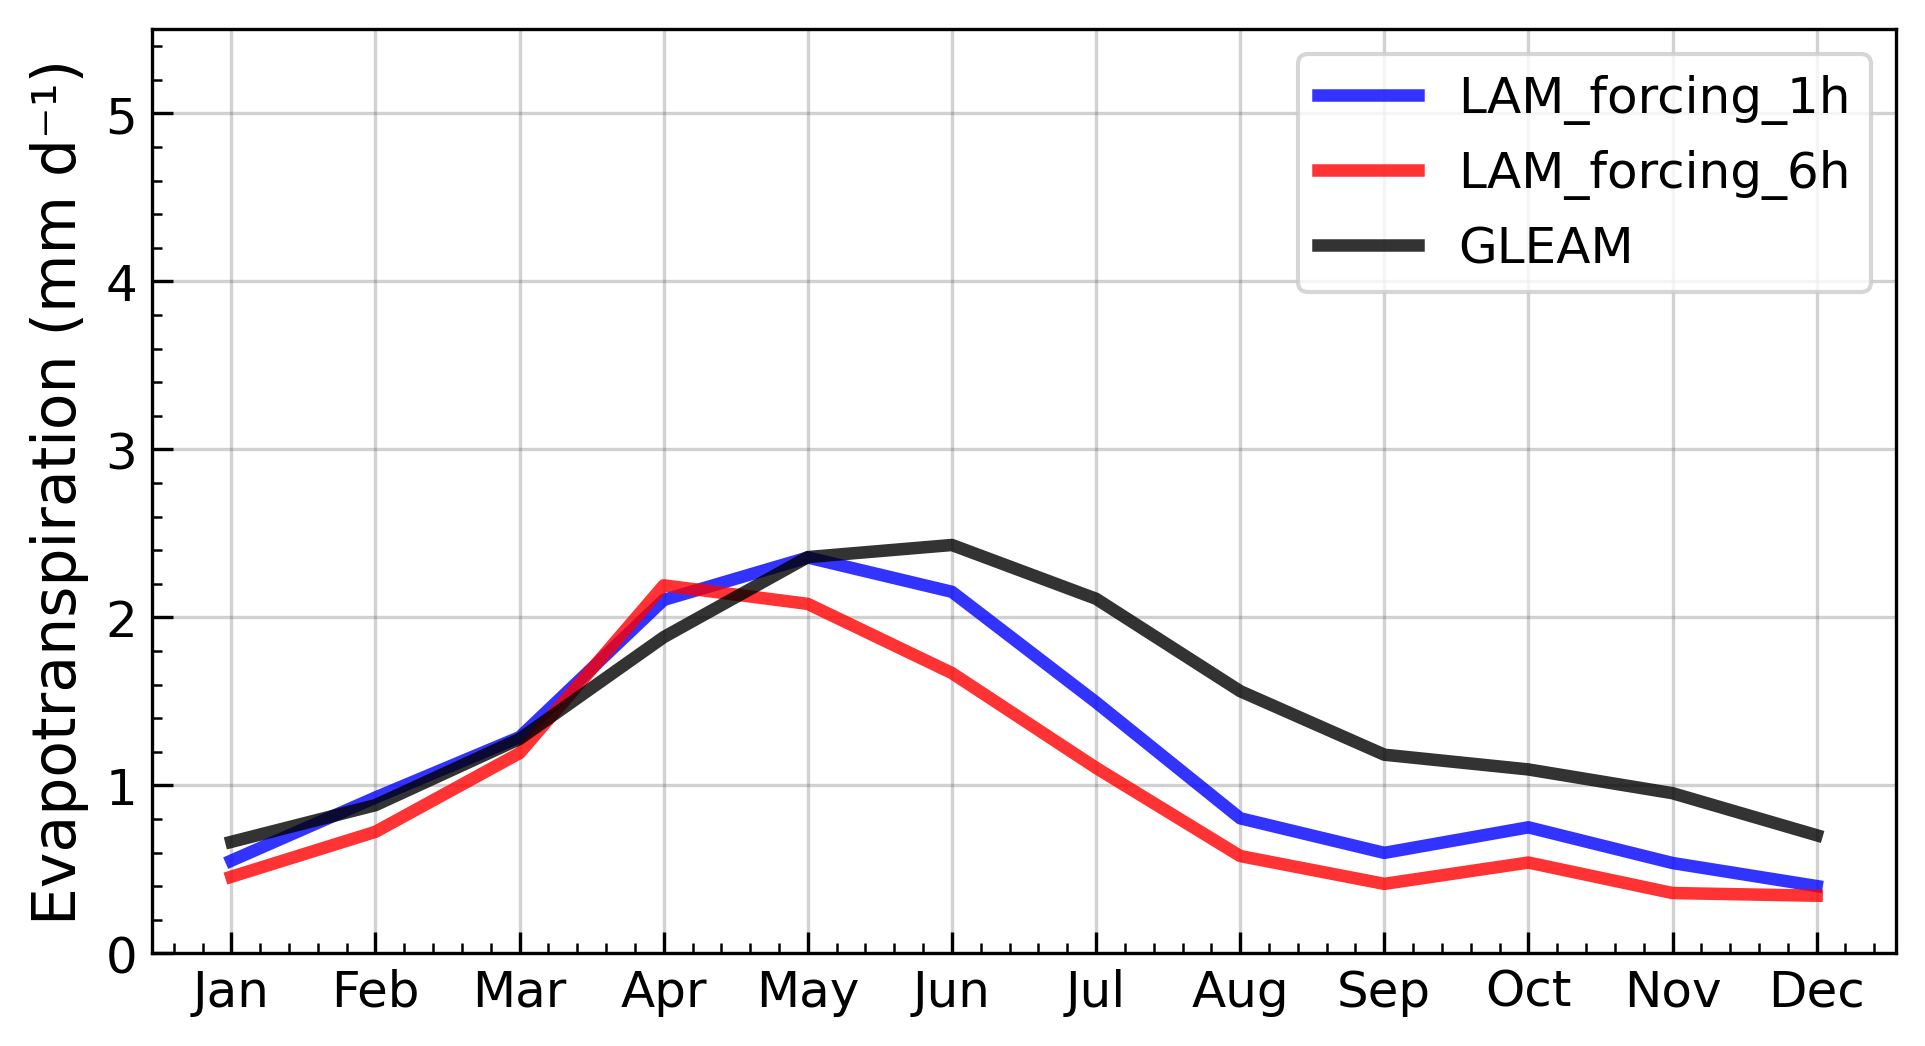
\includegraphics[width=\textwidth]{images/chap4/forcing_sampling_freq/IP_seasonal_cycle_evap.png}
    \end{subfigure}
    \caption{Mean seasonal cycle of precipitation and evapotranspiration, on average over the Iberian Peninsula, for the LAM forced with hourly (blue) and 6-hourly (red) forcing data, and the GPCC and GLEAM products (2013).}
    \label{fig:forcing_sampling_freq_SC}
\end{figure}

Although this study only focused on a single year, it revealed that the model is sensitive to the sampling frequency of the forcing file. The inconsistencies in the transition zone, attributed to discrepancies between the ERA5 forcing and LMDZ physics, are strengthened when using 6-hourly data, which contributes to the degradation of model performance for precipitation and ET over the Iberian Peninsula.

\clearpage

\section{Chapter conclusions}

To identify an appropriate simulation setup for the study, the sensitivities of the LAM to the size of the domain and the choice of lateral forcing (both its source and sampling frequency) were analysed. They revealed an inconsistent behaviour of the LAM in the transition zone when forced by ERA5 data, in particular unexpectedly low cloud cover and precipitation. These biases were attributed to discrepancies between the physics used to produce the ERA5 reanalysis and the LMDZ physics, which keep the large-scale condensation scheme from forming clouds and precipitation properly.
These analyses also showed that this inconsistent behaviour in the transition zone can have impacts in the central part of the domain, and in particular over the Iberian Peninsula. Using larger domains does not make these inconsistencies disappear but limits their influence over the Peninsula since the transition zone is futher away.

Simulations with forced with outputs from a global ICOLMDZOR simulation were compared to the initial setup with forcing data from ERA5 and showed large improvements in the consistency of the model in the transition zone. These findings confirmed that in the transition zone, the model is sensitive to the choice of the forcing data, and identified a possibly better forcing source for future studies with the LAM. However, with this setup, the inherent biases of the ICOLMDZOR model are stronger  in the central zone, which limits the improvements in performance over the Iberian Peninsula.

Sensitivity experiments to look into the impact of the forcing file sampling frequency were also conducted and showed that using 6-hourly ERA5 data for the lateral forcing instead of hourly data amplifies the biases in the transition zone, and degrades performance in the rest of the domain for precipitation and ET. This analysis was conducted with the idea that 6-hourly forcing data could be used for future climate simulation but this option was eventually discarded for technical reasons and all simulations in the rest of this manuscript were run using hourly forcing data.

Although simplifications were made due to technical and time constraints, several dependencies of the ICOLMDZOR LAM on the choice of the domain and forcing data were identified. This work is of high interest for the IPSL modelling community since the LAM is a recent tool, still in development, that is expected to be used in a more and more regional modelling and parameterization development studies.
